\documentclass[a4paper, 12pt]{article}

\input{packages.tex}
\input{commands.tex}
\input{colors.tex}
\input{format.tex}
\setdefaultlanguage{latvian}
\setotherlanguage{english}
\sisetup{output-decimal-marker={,}}
% \titleformat{\subsubsection}{\normalfont\setstretch{1}\hyphenpenalty=10000\fontsize{12}{15}\selectfont\bfseries}{}{0pt}{}
% \titleformat{\paragraph}[runin]{\normalfont\fontsize{12}{15}\selectfont\bfseries}{}{0pt}{}
% \titleformat{\subsubsection}
%     {\fontsize{13}{16}\bfseries}
%     {\thesubsubsection}
%     {2mm}
% \titleformat{\paragraph}[runin]
%     {\fontsize{12}{15}\bfseries}
%     {\theparagraph}
%     {2mm}
%     {\capitalisewords}
% \setcounter{secnumdepth}{2}
% \setcounter{tocdepth}{4}
\DeclareCaptionLabelFormat{lvfigure}{#2. att.}
\DeclareCaptionLabelFormat{lvtable}{#2. tabula}
\captionsetup[figure]{labelformat=lvfigure,labelsep=space}
\captionsetup[table]{labelformat=lvtable}
\DeclareFieldFormat{pages}{-- #1 lpp.}
\AtBeginDocument{\selectlanguage{latvian}% Latvian word breaks generated from Janis Vilims, hyph-lv.tex (2005).
% Source: https://github.com/hyphenation/tex-hyphen (LGPL 2.1 / GPL 2+).
\hyphenation{
abbre-via-tions
abo-ve
abs-tract
abs-trak-ci-jas
ac-ti-ve
adap-tī-vi
adap-tī-vu
addcon-tentsli-ne
addsu-per-vi-sor
ad-justbox
ad-re-se
ad-re-ses
ad-re-sē
ad-re-šu
ad-van-ced
ag-rī-nā-ka-jiem
ag-rī-nās
ai-nas
ai-nās
aiz-stāj
aiz-stā-jot
aiz-stāt
aiz-stā-vē-ša-nai
aiz-sā-ku-mi
aiz-tu-res
aiz-ņem-to
ak-la-jās
ak-ti-vi-tā-te
ak-ti-vi-tā-tes
ak-ti-vi-tā-ti
ak-ti-vi-zē-tās
ak-ti-vā-ci-jas
ak-ti-vā-ci-ju
ak-ti-vā-ci-jām
ak-tuāls
ak-tī-vas
ak-tī-vie
ak-tī-vo
ak-tī-vos
ak-tīvs
ak-tī-vu
aku-mu-la-to-ra
aku-mu-la-to-ru
al-go-rit-mi
al-go-rit-miem
al-go-rit-mis-kais
al-go-rit-mis-ko
al-go-rit-mis-kos
al-go-rit-mis-kā
al-go-ritmu
al-ter-na-tī-va
al-ter-na-tī-vai
al-ter-na-tī-vi
al-ter-na-tī-vām
ana-li-zē-jot
ana-li-zēt
ana-lī-tis-kais
ana-lī-tis-ka-jos
ana-lī-tis-ki
ana-lī-tis-kie
ana-lī-tis-ko
ana-lī-tisks
ana-lī-tis-ku
ana-lī-tis-kus
ana-lī-tis-kās
ana-lī-ze
ana-lī-zes
an-gļu
ano-tā-ci-ja
ap-akš-ko-pas
ap-akš-ko-pās
ap-akš-no-da-ļā
ap-ara-tū-ra
ap-ara-tū-ras
ap-ara-tū-ru
ap-ara-tū-rā
ap-ga-ba-la
ap-gal-vo-ju-mus
ap-grū-ti-na
ap-gū-ta
ap-ie-ša-nai
ap-jo-ma
ap-jo-mam
ap-joms
ap-jo-mu
ap-ko-po-tas
ap-ko-po-ti
ap-kārtska-ta
ap-la-mi
ap-lie-ci-not
ap-lū-ko
ap-lū-kot
ap-lū-ko-ta
ap-lū-ko-tie
ap-lū-ko-to
ap-lū-ko-tā
ap-mai-nī-tas
ap-mai-ņai
ap-mā-ca
ap-mā-cāms
ap-mā-cā-mu
ap-mā-cā-mus
ap-mā-cā-mām
ap-mā-cī-ba
ap-mā-cī-bai
ap-mā-cī-bas
ap-mā-cī-bu
ap-mā-cī-bā
ap-mā-cī-tais
ap-mā-cī-ti
ap-mā-cī-tie
ap-mā-cī-tos
ap-mā-cīts
ap-plau-se
ap-pli-ca-tions
ap-prox
ap-rak-sta
ap-rak-stī-ja
ap-rak-stīt
ap-rak-stī-ta
ap-rak-stīts
ap-rok-si-mā-ci-ja
ap-rok-si-mā-ci-jai
ap-rok-si-mā-ci-jas
ap-rok-si-mā-ci-ju
ap-rok-si-mē
ap-rok-si-mēt
ap-rok-si-mē-tas
ap-rē-ķi-na
ap-rē-ķi-ni
ap-rē-ķi-niem
ap-rē-ķi-nos
ap-rē-ķi-nu
ap-rē-ķi-nus
ap-rē-ķi-nāt
ap-rē-ķi-nā-ta
ap-rē-ķi-nā-ša-na
ap-rē-ķi-nā-ša-nai
ap-rī-kots
ap-stip-ri-na
ap-stip-ri-nu
ap-stip-ri-nā-ja
ap-stip-ri-nā-jums
ap-stip-ri-nā-ta
ap-strā-de
ap-strā-dei
ap-strā-des
ap-strā-di
ap-strā-dā
ap-strā-dāt
ap-strā-dā-to
ap-stāk-ļos
ap-tu-ve-ni
ap-tver
ap-vie-no
ap-vie-no-jot
ap-vie-no-ju-ma
ap-vie-not
ap-vie-no-ta
ap-vie-no-ti
ap-vie-no-tā
ap-vie-no-ša-na
ap-vie-no-ša-nas
ap-vie-no-ša-nu
ap-zī-mē
ap-zī-mē-jot
archi-tectu-re
ar-gu-ments
ar-hi-tek-tū-ra
ar-hi-tek-tū-rai
ar-hi-tek-tū-ras
ar-hi-tek-tū-ru
ar-hi-tek-tū-rā
ar-hi-tek-tū-rām
ar-hi-tek-tū-rās
arit-mē-ti-kā
arit-mē-tis-ko
arit-mē-tis-kām
ar-ticle
ar-vien
asin-hro-no
asin-hro-nu
asin-hro-nus
as-pek-tiem
as-pek-tus
at-bal-sta
at-bal-stam
at-bal-stī-tu
at-bild
at-bilst
at-bil-stot
at-bil-sto-ša
at-bil-sto-šas
at-bil-sto-ši
at-bil-sto-šo
at-bil-sto-šu
at-bil-stu
at-bil-stī-bai
at-da-lā-miem
at-da-ri-na
at-da-ri-nāt
at-da-ri-nā-tu
at-grie-žas
at-ies-ta-tī-ta
at-ies-ta-tī-ša-nas
at-ies-ta-tī-ša-nu
at-jau-ni-na
at-jau-ni-nā-ti
at-jau-ni-nā-to
at-jau-ni-nāts
at-jau-ni-nā-tu
at-jau-ni-nā-ša-nas
at-jau-ni-nā-ša-nu
at-jau-no-tu
at-jau-no-ša-nās
at-ka-rī-ba
at-ka-rī-bā
at-ka-rī-ga
at-ka-rī-gas
at-ka-rīgs
at-ka-rī-gā
at-klā-tā
at-kār-to
at-kār-to-ta
at-kār-to-tas
at-kār-to-ti
at-kār-tots
at-kār-to-tu
at-li-ku-ma
at-mi-ņa
at-mi-ņai
at-mi-ņas
at-mi-ņu
at-mi-ņā
at-pa-kaļ
at-pa-ka-ļiz-pla-tī-ša-na
at-pa-liek
at-pa-lie-kot
at-pa-zī-ša-nas
at-pa-zī-ša-nu
at-ras-ti
at-ri-si-nā-ju-miem
at-ri-si-nā-jums
at-ri-si-nā-ta
at-ro-da-ma
at-ro-do-ties
at-se-viš-ķa-jiem
at-se-viš-ķi
at-se-viš-ķie
at-se-viš-ķiem
at-se-višķs
at-se-viš-ķu
at-se-viš-ķām
at-spo-gu-ļo
at-tie-cas
at-tie-cī-ba
at-tie-cī-bas
at-tie-cī-bā
at-tie-cī-ga-jās
at-tie-cī-gi
at-tie-cī-gie
at-tā-lu-mam
at-tā-lums
at-tā-lu-mu
at-tē-la
at-tē-li
at-tē-liem
at-tē-lo
at-tē-lo-ju-mu
at-tē-lo-tas
at-tē-lots
at-tē-lu
at-tēlvei-do-ša-nas
at-tē-lā
at-tīs-tī-ba
at-tīs-tī-bu
at-tīs-tī-ju-šies
at-va-si-nā-ju-mu
at-vei-dot
at-vieg-lo
at-vieg-lo-tu
at-vieg-lo-ša-nai
at-šķirt
at-šķir-tu
at-šķi-rī-ba
at-šķi-rī-bas
at-šķi-rī-bu
at-šķi-rī-bā
at-šķi-rī-gas
at-šķir-ša-nai
au-di-to-ri-ja
augst-as
augst-ums
augst-u-mu
augst-u-mus
augst-ā-ka
augst-ā-kas
augst-ā-ko
augst-āks
augst-ā-ku
aug-šas
au-to-ma-ti-zē-ta
au-to-ma-ti-zē-tas
au-to-ma-ti-zē-tā
au-to-ma-ti-zē-tām
au-to-mo-bi-lis
au-to-mo-bi-ļu
au-to-mo-ti-ve
au-to-mā-tis-kās
au-to-no-ma-jos
au-to-no-ma-jās
au-to-no-mous
au-to-no-mās
bal-stās
bal-stī-ta
bal-stī-tai
bal-stī-tais
bal-stī-ta-jiem
bal-stī-tas
bal-stī-ti
bal-stī-tie
bal-stī-tiem
bal-stī-to
bal-stī-tos
bal-stīts
bal-stī-tu
bal-stī-tus
bal-stī-tā
bal-stī-tām
bal-stī-tās
bar-dow
ba-ro-ša-nas
bas-ler
bas-lerbla-ze
be-gin
be-low
bfse-ries
bi-bin-toc
bib-lio-tē-ku
bie-ži
bie-žu-mu
bi-nā-ri
bi-nā-riem
bi-nā-ro
bi-nārs
bi-nā-ru
bi-nā-rus
bi-nā-rā
bi-nā-rās
bio-lo-ģis-ki
bio-lo-ģis-ko
bio-lo-ģis-kā
bio-lo-ģis-kās
bi-tiem
bla-kus
bla-ze
blo-ka
blo-ki
blo-kiem
blo-kos
blo-ku
blue-hi-ve
blī-vas
blī-viem
blī-vu
blī-vām
bottomru-le
brauk-ša-na
brauk-ša-nas
brī-dim
brī-dī
brīv-piek-ļu-ves
bu-dže-tu
bu-fe-ri
bu-fe-riem
bu-fe-rē-ša-nai
bur-den
bā-zes
bū-tis-ka
bū-tis-ki
bū-tisks
cal-tech
cap-tion
cap-tion-se-tup
ca-ses
caur-lai-dī-ba
caur-lai-dī-bu
cen-ter
cen-te-ring
cen-terli-ne
cen-tra
cen-šas
chak-ra-borty
cha-ract
cie-ši
cie-šāk
cie-šā-ka
ci-far
cik-lā
cil-pa
cil-vē-ka
ci-pa-ru
circle-dast
ci-tas
ci-te-num
ci-tiem
ci-tos
ci-tās
clear-doub-le-page
clear-page
cmid-ru-le
co-lors
co-lumnwidth
com-pa-re
coor-di-na-tes
cor-dic
cor-do-ne
corra-di
csu-se
da-lī-ša-na
dar-ba
dar-bam
dar-bi
dar-biem
dar-bi-nā-mas
dar-bi-nā-ta
dar-bi-nā-ša-nu
dar-bo-jas
dar-bo-jo-ties
dar-bos
darbplūs-ma
dar-bu
dar-bus
dar-bā
dar-bī-bai
dar-bī-bas
da-tiem
da-torre-dzes
da-torre-dzē
da-torzi-nāt-nes
da-torzi-nāt-ņu
da-tos
da-tums
da-tus
dau-dziem
daudzka-nā-lu
daudzlī-me-ņu
daudzpro-ce-so-ru
daudzslā-ņu
daudz-so-lošs
dau-dzuz-de-vu-mu
dau-dzām
da-ļai
da-ļām
da-ļās
da-žos
da-žus
da-žā-das
da-žā-di
da-žā-diem
da-žā-dos
da-žā-du
da-žā-dus
da-žā-dām
da-žā-dās
da-žām
da-žās
de-ci-mal
dec-la-re-cap-tionla-belfor-mat
dec-la-re-fieldfor-mat
de-co-der
de-fi-nē
de-fi-nēt
de-fi-nēts
deg-ree
de-ko-dē-ta
de-ko-dē-tā-ja
del-ta
de-mons-trē
de-mons-trē-ja
de-mons-trē-jot
de-mons-trē-ta
de-mons-trēts
de-mons-trē-tu
den-se-net
dep-re-si-ja
des-mit
de-ta-li-zā-ci-jas
de-ta-li-zē-tas
de-ta-li-zē-ti
de-ta-li-zē-to
de-ta-li-zē-tā-ku
de-ta-ļām
de-tec-tion
de-tec-tions
de-tek-to-ra
de-tek-to-riem
de-tek-tors
de-tek-tē-ju-ma
de-tek-tē-ju-mus
de-tek-tē-ta-jam
de-tek-tē-tu
de-tek-tē-ša-na
de-tek-tē-ša-nai
de-tek-tē-ša-nas
de-tek-tē-ša-nu
de-tek-tē-ša-nā
de-ter-mi-nē-tai
de-ter-mi-nēts
de-ter-mi-nē-tu
de-vu-ši
dia-pa-zo-nu
dia-pa-zo-nā
di-fe-ren-ciāl-vie-nā-do-ju-ma
di-fe-ren-ciāl-vie-nā-do-ju-mu
di-fe-ren-ciāl-vie-nā-do-ju-mus
di-gi-tā-lais
di-gi-tā-la-jā
di-gi-tā-lo
di-gi-tā-lā
di-gi-tā-lās
dil-ša-nas
di-men-si-ja
di-men-si-jas
di-men-si-jā
di-men-si-jām
di-na-mi-ka
di-na-mi-kas
di-na-mi-ku
di-na-mis-kais
di-na-mis-ko
di-na-mis-kā
di-na-mis-kās
di-ra-ka
discre-te
dis-kre-ti-zā-ci-jas
dis-kre-ti-zā-ci-ju
dis-krē-ta
dis-krē-tais
dis-krē-tas
dis-krē-tiem
dis-krē-to
dis-krē-tos
dis-krē-tu
dis-krē-tus
dis-krē-tā
di-vas
div-nie-ka
div-por-tu
divslā-ņu
di-vus
di-vās
do-cu-ment
do-cu-mentclass
dok-to-ra
dok-to-rants
do-mi-nē
do-mēnspe-ci-fis-ka
do-mē-nu
do-tai
do-tas
drai-ve-ra
drai-ve-ri
dro-šas
dzi-ļais
dzi-ļa-jiem
dzi-ļas
dzi-ļi
dzi-ļie
dzi-ļiem
dzi-ļo
dzi-ļos
dzi-ļu-ma
dzi-ļu-mam
dzi-ļu-mu
dzi-ļus
dzi-ļā
dzi-ļā-kas
dzi-ļā-ki
dzi-ļā-kie
dzi-ļā-ku
dzi-ļā-kus
dzi-ļā-kām
dzi-ļās
dār-ga
dār-gas
dār-gu
dār-gām
dīk-stā-ve
dīk-stā-ves
dīk-stā-vē
eco-mo-bi-lity
efek-ti-vi-tā-tes
efek-ti-vi-tā-ti
efek-tī-va
efek-tī-vai
efek-tī-vas
efek-tī-vi
efek-tīvs
efek-tī-vu
efek-tī-vā
efek-tī-vā-kas
efek-tī-vā-ku
ei-le-ra
ek-spe-ri-men-ti
ek-spe-ri-men-tu
ek-spe-ri-men-tā-lais
ek-spe-ri-men-tā-la-jā
ek-spe-ri-men-tā-li
ek-spe-ri-men-tā-lie
ek-spe-ri-men-tā-lu
ek-spe-ri-men-tā-lā
ek-spo-nen-ciā-li
ek-spo-nen-ciā-lo
ek-spo-nen-ciā-lās
ek-vi-va-len-ta
ek-vi-va-len-tiem
ek-vi-va-len-to
ek-vi-va-len-tu
ek-vi-va-len-tām
elas-tī-ba
elas-tī-bu
elas-tī-gu
electri-cal
electro-nics
elek-tris-kās
elek-tro-ni-ka
elek-tro-ni-kas
ele-men-ti
ele-men-tiem
el-lip-se
em-bedded
enco-der
ener-goe-fek-ti-vi-tā-te
ener-goe-fek-ti-vi-tā-tei
ener-goe-fek-ti-vi-tā-tes
ener-goe-fek-ti-vi-tā-ti
ener-goe-fek-tī-vam
ener-goe-fek-tī-vas
ener-goe-fek-tī-vu
ener-goe-fek-tī-vus
ener-goe-fek-tī-vā
ener-goe-fek-tī-vā-kais
ener-goe-fek-tī-vām
ener-ģi-ja
ener-ģi-jai
ener-ģi-jas
ener-ģi-ju
ener-ģi-jā
ener-ģē-ti-kas
en-su-ring
enu-me-ra-te
equa-tion
eso-ša-jos
eso-šas
eso-šie
eso-šo
eso-šām
eso-šās
eta-lon-mar-ķē-ju-ma
eta-lon-tes-ta
eta-lon-tes-tiem
eta-lon-tes-tos
eta-lon-tes-tā
eta-lo-nu
eu-ler
eu-ro-pe
eu-ro-pean
eva-lua-tion
evo-lu-cio-nā-rās
evo-lu-cio-nē-jo-ša
exe-cu-tion
fa-culty
fak-tis-ki
fak-to-riem
fa-kul-tā-te
fi-gu-re
fik-sē-tiem
fik-sē-tu
fik-sē-tā
fil-tra
fi-zis-kiem
fo-kā-lo
fontsi-ze
footno-te
footno-te-si-ze
fo-reach
for-mas
for-mat
for-mu
for-mā-li
for-mā-lie
for-mā-tā
fo-to-dio-de
frek-ven-ce
frek-ven-ci
fun-kci-jas
fun-kci-ju
fun-kci-jām
fun-kcio-nā-lo
fur-ber
fu-tu-re
fā-zes
ga-bo-ra
ga-dī-ju-mos
ga-dī-jums
ga-dī-ju-mu
ga-dī-ju-mā
gais-mas
gal-va
gal-vai
gal-vas
gal-ve-nais
gal-ve-nie
gal-ve-no
gal-ve-no-kārt
gal-ve-nā
gal-ve-nās
gal-vām
ga-lī-go
ga-ro-zas
ga-rums
ge-for-ce
gei-ger
getsu-per-vi-sor-deg-ree
getsu-per-vi-sor-na-me
getsu-per-vi-sor-po-si-tion
gewal-tig
gla-bā
gla-bā-ja-mo
gla-bā-jot
gla-bāt
gla-bā-ti
gla-bā-ša-na
gla-bā-ša-nai
gla-bā-ša-nas
gla-bā-ša-nu
glo-bā-lo
glo-bā-lā
glsla-bel
goodfel-low
gra-fis-kās
gru-pa
grā-da
grā-du
grū-ti
grū-tī-bas
gup-ta
gā-jējs
gā-jē-ju
gā-jē-jus
ha-bil
haksli-ja
hea-ding
hei-darpour
he-te-ro-gē-nām
hib-rī-da
hib-rī-dai
hi-per-pa-ra-met-rus
his-tog-ram-mu
hodžki-na
ho-ri-zon
ho-ri-zon-tā-lo
ho-rowitz
hyphen-pe-nalty
idea-li-zē-to
iden-ti-fi-cē-jot
iden-ti-fi-cē-to
iden-ti-fi-ka-tors
iden-ti-tā-ti
ie-da-la
ie-dves-mas
ie-dves-mo-tu
ie-dves-mo-tus
ie-eja
ie-ejas
ie-eju
ie-gul-dī-ju-ma
ie-gul-dī-ju-mam
ie-gul-dī-ju-mos
ie-gul-dī-jums
ie-gul-dī-ju-mu
ie-gul-ta-jā
ie-gul-ta-jām
ie-gul-ta-jās
ie-gul-tā
ie-gul-tām
ie-gul-tās
ie-gu-vums
ie-gu-vu-mu
ie-gūst
ie-gūs-tot
ie-gūt
ie-gū-ta-jai
ie-gū-ta-jiem
ie-gū-ta-jos
ie-gū-ta-jām
ie-gū-ti
ie-gū-to
ie-gūts
ie-gū-tu
ie-gū-tā
ie-gū-tām
ie-gū-tās
ie-gū-ša-na
ie-gū-ša-nai
ie-kļau-ta
iek-šā
iek-šē-jai
iek-šē-jo
iek-šē-jos
iek-šē-jā
iek-šē-jās
ie-lā-dei
ie-lā-di
ie-priekš
ie-priek-šē-jo
ie-priek-šē-jos
ie-priek-šē-jā
ie-rak-stos
ie-rak-stī-ti
ie-rak-stī-ša-nai
ie-ro-be-žo
ie-ro-be-žo-ju-mi
ie-ro-be-žo-ju-miem
ie-ro-be-žo-ju-mu
ie-ro-be-žo-ju-mus
ie-ro-be-žo-ta
ie-ro-be-žo-tas
ie-ro-be-žots
ie-ro-be-žo-tu
ie-rī-ce
ie-rī-ces
ie-rī-ci
ie-rī-cēs
ie-sniegts
ie-spiests
ie-spē-ja-mais
ie-spē-ja-mi
ie-spē-ja-mās
ie-spē-ja-mī-ba
ie-spē-ja-mī-bu
ie-spē-jas
ie-spē-ju
ie-sta-tī-tas
ie-sta-tīts
ie-tau-pī-ju-mi
ie-tau-pī-ju-mu
ie-tei-ku-mi
ie-tek-me
ie-tekmi
ie-tek-mē
ie-til-pī-ba
ie-til-pī-bu
ie-tva-ra
ie-tva-riem
ie-tva-ros
ie-tvars
ie-tva-ru
ie-tva-rus
ie-tva-rā
ie-tver
ie-tve-ro-ša-jiem
ie-tve-ro-šie
ie-tve-ro-šo
ie-tve-ro-šos
ie-tve-ro-šā
ie-tvert
ie-tvē-ra
ie-vads
ie-viest
ie-vie-to-jot
ie-vie-to-ti
ie-vie-ša-na
ie-vie-ša-nai
ie-vie-ša-nas
ie-vē-ro-ja-mas
ie-vē-ro-ja-mi
ie-vē-ro-jams
ie-vē-ro-ja-mu
ie-vē-ro-ja-mus
ie-vē-ro-jot
ie-vē-ro-jo-šu
ik-reiz
ilgter-mi-ņa
il-gu-ma
il-gums
ilus-trē
ilus-trē-tas
ilus-trēts
im-pul-sa
im-pul-sam
im-pul-si
im-pul-siem
im-pulss
im-pul-su
im-pul-sus
inclu-deg-rap-hics
inclu-desvg
in-dek-sa
in-dek-sam
in-dek-su
in-dek-sus
in-dek-sē
in-dex
in-di-vi-duā-lo
in-fe-ren-ce
in-fe-ren-cei
in-fe-ren-ces
in-fe-ren-ci
in-fe-ren-cē
in-for-mā-ci-ja
in-for-mā-ci-jas
in-for-mā-ci-ju
in-for-mā-ci-jā
in-fras-truk-tū-ru
in-ner
in-sti-tu-te
in-sti-tūts
in-sti-tū-tā
in-teg-rā-ci-ja
in-teg-rā-ci-jas
in-teg-rā-ci-ju
in-teg-rā-lā
in-teg-rā-lās
in-teg-rē
in-teg-rē-jot
in-teg-rē-jo-šais
in-teg-rē-jo-šiem
in-teg-rē-jo-šā
in-teg-rēt
in-teg-rē-ti
in-teg-rēts
in-teg-rē-ša-nas
in-te-lek-ta
in-te-lek-tam
in-te-lekts
in-te-lek-tuā-lo
in-tel-li-gen-ce
in-tel-li-gent
in-te-re-si
in-terp
in-ter-po-lē-tā
in-ter-vā-la
in-ter-vā-li
in-ter-vā-los
in-ter-vāls
in-ter-vā-lā
in-tro-duction
in-že-nie-ri-jas
ite-mi-ze
ite-rā-ci-jai
ite-rā-ci-ju
iz-ai-ci-nā-jums
iz-celt
iz-dev-nie-cī-ba
iz-de-vī-gas
iz-de-vīgs
iz-eja
iz-ejas
iz-eju
iz-ejām
iz-hi-ke-vich
iz-klie-dē-tai
iz-klie-dē-tiem
iz-klie-dē-tu
iz-klie-dē-tā
iz-klās-tot
iz-klās-tī-ta
iz-lai-des
iz-le-co-šām
iz-lā-dē-jas
iz-mai-ņas
iz-mai-ņām
iz-mak-sas
iz-mak-su
iz-mak-sām
iz-man-to
iz-man-to-jot
iz-man-to-jums
iz-man-to-ju-mu
iz-man-tot
iz-man-to-ta
iz-man-to-tais
iz-man-to-ta-jai
iz-man-to-tas
iz-man-to-ti
iz-man-to-tie
iz-man-to-tiem
iz-man-tots
iz-man-to-tu
iz-man-to-tā
iz-man-to-tās
iz-man-to-ša-na
iz-man-to-ša-nai
iz-man-to-ša-nu
iz-mē-ra
iz-mē-riem
iz-mērs
iz-mē-ru
iz-mē-rus
iz-mē-rī-ta
iz-mē-rī-tais
iz-mē-rī-ta-jām
iz-mē-rī-tie
iz-mē-rī-to
iz-mē-rī-tu
iz-mē-rī-tās
iz-pil-da
iz-pil-de
iz-pil-des
iz-pil-di
iz-pil-dot
iz-pil-dīt
iz-pil-dī-ti
iz-pil-dīts
iz-pla-tī-tā
iz-pla-tī-ša-nas
iz-pla-tī-ša-nās
iz-prat-ne
iz-prat-nei
iz-pē-tei
iz-pē-ti
iz-pē-tīt
iz-pē-tī-tu
iz-rai-sīt
iz-sa-kot
iz-se-ko-tājs
iz-se-ko-ša-nas
iz-skaid-ro-ja-ma
iz-ska-tī-ša-nai
iz-slēg-tu
iz-sta-ro
iz-sta-ro-ti
iz-strā-de
iz-strā-dei
iz-strā-des
iz-strā-di
iz-strā-dā-jis
iz-strā-dāt
iz-strā-dā-ta-jam
iz-strā-dā-ti
iz-strā-dā-tie
iz-strā-dāts
iz-strā-dā-tā
iz-teik-sme
iz-teik-smi
iz-teikt
iz-teik-tā-kas
iz-vai-ro-ties
iz-vai-rī-ties
iz-vai-rī-tos
iz-vei-de
iz-vei-dei
iz-vei-des
iz-vei-do
iz-vei-do-jot
iz-vei-do-ti
iz-vie-to-ta
iz-vie-to-tai
iz-vie-to-ša-nas
iz-vir-zī-ti
iz-vir-zīts
iz-vē-las
iz-vē-le
iz-vē-lei
iz-vē-les
iz-vē-li
iz-vē-lo-ties
iz-vē-lē-ti
iz-vē-lē-tiem
iz-vē-lē-ties
iz-vē-lēts
iz-vē-lē-tu
iz-vē-lē-tām
iz-vēr-tēt
iz-vēr-tē-tu
iz-šķirtspē-ja
iz-šķirtspē-jas
iz-šķirtspē-ju
iži-ke-vi-ča
jau-da
jau-das
jau-du
jauk-ta
jauk-tu
jau-na
jau-nie
jau-nu
jau-nā-ka-jos
jau-nā-kie
jau-nā-kās
jeb-ku-ras
jet-son
jop-ro-jām
jos-las
jou-le
jus-ti-fi-ca-tion
ju-tī-ba
ju-tī-bu
jā-ap-rē-ķi-na
jā-at-zī-mē
jā-ko-dē
jā-no-rā-da
jā-no-vēr-tē
jā-pār-vei-do
jā-uz-ska-ta
jā-veic
jā-ņem
ka-di-ķis
kad-ri
kad-riem
kad-ru
kal-po
ka-me-ru
ka-me-rām
ka-nā-la
ka-nā-lam
ka-nā-li
ka-nā-liem
ka-nā-lu
ka-nā-lus
ka-nā-lā
ka-pa-ci-tā-tei
ka-pa-ci-tā-ti
kar-te
kar-tei
kar-tes
kar-ti
kar-tē
kar-tēm
kar-tēs
kar-tē-tu
kar-tē-ša-nu
kar-šu
kas-kā-dē
ka-te-go-ri-ja
ka-te-go-ri-jā
kat-ra
kat-rai
kat-ram
kat-ru
kat-rā
ka-vē-ja
kin-tex
kit-ti
kla-se
kla-sei
kla-ses
kla-si-fi-cē-ja-mu
kla-si-fi-cē-to
kla-si-fi-ka-tors
kla-si-fi-kā-ci-ja
kla-si-fi-kā-ci-jai
kla-si-fi-kā-ci-jas
kla-si-fi-kā-ci-ju
kla-sēm
kla-šu
klāt-būt-ni
ko-do-la
ko-do-liem
ko-dols
ko-do-lu
ko-do-lus
ko-do-lā
ko-dē-jot
ko-dē-ta
ko-dē-tas
ko-dē-ti
ko-dē-to
ko-dē-tos
ko-dē-tu
ko-dē-tus
ko-dē-tā-ja
ko-dē-tā-ju
ko-dē-tās
ko-dē-ša-na
ko-dē-ša-nai
ko-dē-ša-nas
ko-dē-ša-nu
koe-fi-cien-ti
koe-fi-cients
koe-fi-cien-tu
kohleā-rie
kok-vei-da
ko-lon-nu
ko-ma-ta
kom-pak-tos
kom-pakts
kom-pen-sēt
kom-plek-sās
kom-ple-men-tā-rā
kom-po-nen-tu
kom-po-nen-tus
kom-pro-mi-si
kom-pro-miss
kom-pro-mi-su
kon-cen-trē-jas
kon-cep-ci-ja
kon-cep-ci-jas
kon-den-sa-to-ra
kon-den-sa-tors
kon-den-sa-to-ru
kon-fi-gu-rā-ci-ja
kon-fi-gu-rā-ci-jai
kon-fi-gu-rā-ci-jas
kon-fi-gu-rā-ci-ju
kon-fi-gu-rā-ci-jām
kon-fi-gu-rē-ja-ma
kon-fi-gu-rē-ja-mi
kon-fi-gu-rē-jams
kon-fi-gu-rē-ja-mu
kon-fi-gu-rē-ja-mus
kon-fi-gu-rē-ja-mā
kon-fi-gu-rēt
kon-fi-gu-rē-ti
kon-krē-ti
kon-ku-rēt-spē-jī-ga
kon-ku-rēt-spē-jī-gu
kon-sek-ven-tam
kon-stan-tas
kon-stan-te
kon-stan-tes
kon-stan-ti
kon-vei-je-ra
kon-vei-je-ri
kon-vei-je-ri-zē-ta
kon-vei-je-ri-zē-tas
kon-vei-je-ri-zēts
kon-vei-je-ri-zē-tu
kon-vei-jers
kon-vei-je-ru
kon-vo-lu-cio-nā-lais
kon-vo-lu-cio-nā-la-jiem
kon-vo-lu-cio-nā-li
kon-vo-lu-cio-nā-lie
kon-vo-lu-cio-nā-liem
kon-vo-lu-cio-nā-lo
kon-vo-lu-cio-nā-los
kon-vo-lu-cio-nā-lu
kon-vo-lu-cio-nā-lā
kon-vol-vēts
kon-vo-lū-ci-ja
kon-vo-lū-ci-jai
kon-vo-lū-ci-jas
kon-vo-lū-ci-ju
kon-vo-lū-ci-jām
koor-di-nā-tas
koor-di-nā-tu
koor-di-nā-tām
ko-pai
ko-pas
kop-lie-to-tie
kop-lie-tots
kop-pro-jek-tē-jums
kop-sa-vil-kums
ko-pu-mā
ko-pām
ko-pās
ko-pē-jais
ko-pē-jie
ko-pē-jo
ko-pē-jā
ko-pē-jās
ko-pī-ga
ko-pī-gi
ko-pīgs
ko-pī-gu
ko-pī-gā
kou-sa-na-kis
kri-tis-ki
kri-tis-kiem
kri-tums
krā-su
ku-ras
ku-riem
ku-ros
kvad-rā-tis-kā
kvan-tē
kvan-tē-ta
kvan-tē-ti
kvan-tē-tie
kvan-tē-tu
kvan-tē-tus
kvan-tē-ša-na
kvan-tē-ša-nas
kvan-tē-ša-nu
kā-dēļ
kār-tas
kļu-vu-ši
kļū-da
kļū-dai
kļū-das
kļū-du
la-bel
la-belfor-mat
la-belsep
la-bus
la-bā-ku
lai-ka
lai-ki
lai-kiem
laik-rin-dās
lai-ku
lai-kā
la-pi-ka
lap-pu-šu
lar-ge
las-tpage
la-sī-ša-nai
la-sī-ša-nas
la-ten-tu-ma
la-ten-tu-mi
la-ten-tums
la-ten-tu-mu
lat-vian
lat-vi-jā
lau-kiem
lau-ku
lau-ku-mu
lau-kā
la-vī-nas
leņ-ķis
li-dar
li-do-ju-ma
lie-ci-na
lie-ki
lie-kus
lie-la
lie-lam
lie-la-murs
lie-las
lieljau-das
lie-lo
lie-lu
lie-lu-mu
lie-lā
lie-lā-ka
lie-lā-kas
lie-lā-kiem
lie-lā-ko
lie-lāks
lie-lā-ku
lie-lā-kus
lie-lā-kā
lie-lā-murs
lie-to-ju-ma
lie-to-ju-miem
lie-to-ju-mos
lie-to-jumspe-ci-fis-kā
lie-to-jumspe-ci-fis-kās
lie-to-tā-ja
lie-to-tā-jam
li-nes
li-newidth
li-neā-ra
li-neā-ri
li-neārs
li-neā-rā
li-te-ra-tū-ras
lo-cek-li
lo-cek-lis
lo-cek-ļi
lo-cek-ļu
lo-giem
loi-hi
lo-ka-li-zā-ci-ju
lo-kā-li
lo-kā-lo
lo-kā-lā
lo-ģi-ka
lo-ģi-kai
lo-ģi-kas
lo-ģi-ku
lo-ģis-kais
lo-ģis-ka-jai
lo-ģis-ko
lvfi-gu-re
lvtab-le
lā-di-ņu
lē-mu-mu
lī-dzi-nā-jās
lī-dzi-nās
līdz-sva-ra
līdz-sva-ro
līdz-sva-ro-tu
līdz-sva-ru
līdzvēr-tī-bu
līdzvēr-tī-gai
līdzvēr-tī-gus
lī-dzī-ba
lī-dzī-bas
lī-dzī-ga
lī-dzī-gi
lī-dzī-gā
līk-nes
lī-me-nim
lī-me-nis
lī-me-nī
lī-me-ņa
lī-me-ņos
lī-me-ņu
lī-ni-jas
machi-nes
mai-nās
mai-nī-gai
mai-nī-gais
mai-nī-go
mai-nī-gā
ma-ka-loks
ma-keat-letter
ma-kea-tother
ma-keg-lossa-ries
ma-ke-lowerca-se
ma-keupperca-se
mak-si-mu-ma
mak-si-mums
mak-si-mā-las
mak-si-mā-lo
mak-si-mā-lā
mak-si-mā-lās
ma-lām
ma-nu-factu-ring
ma-nuā-li
mar-ker
mar-ķē-ju-mi
mar-ķē-ju-mus
mar-ķē-ta
mas-kē-ša-nas
mas-kē-ša-nu
ma-sī-vi
ma-sīvs
ma-sī-vus
ma-te-mā-tis-ki
ma-te-mā-tis-ko
ma-zas
ma-zi-nāt
ma-zi-nā-tu
ma-zāk
ma-zā-ka
ma-zā-kas
ma-zā-kos
ma-zā-ku
ma-zā-kās
mccul-loch
mea-su-red
mek-lē-ja-mi
mek-lē-tu
mek-lē-ša-na
mem-bra-ne
mem-brā-na
mem-brā-nas
mem-brā-nu
me-mop
me-to-de
me-to-des
me-to-di
me-to-do-lo-ģi-ja
me-to-do-lo-ģi-jai
me-to-do-lo-ģi-ju
me-to-dēm
met-re
met-ri-ka
met-ri-kas
met-ri-ku
met-ri-kā
me-tā-la
mid-ru-le
mie-ra
mik-ro-kon-trol-le-ra
mik-rop-ro-ce-so-ra
mik-roshē-mas
mik-roshē-mā
mik-ro-viļ-ņu
mil-jo-niem
mil-li
mi-ni-mum
mi-ni-mu-mam
mi-ni-mā-lais
mi-ni-mā-la-jām
mi-ni-mā-lās
mo-bi-la-jos
mo-bi-lity
mo-da-li-tā-tei
mo-da-li-tā-tēm
mo-del
mo-de-li
mo-de-lim
mo-de-lis
mo-de-lē-ta
mo-de-lē-tais
mo-de-lī
mo-der-nā-ka-jiem
mo-der-nā-kās
mo-de-ļa
mo-de-ļi
mo-de-ļiem
mo-de-ļos
mo-de-ļu
mo-de-ļus
mo-di-fi-kā-ci-ja
mo-du-lis
mo-du-ļa
mo-du-ļus
mon-star
moo-re
mo-ti-vē
mul-ti-co-lumn
mul-tiplek-sē-ta
mul-tiplek-sē-tas
mul-tiplek-sēts
mul-tiplek-sē-tā
mul-ti-row
mā-cī-ša-nās
mā-ko-nis
mā-ko-ņa
mā-ko-ņi
mā-ko-ņiem
mā-ko-ņos
mā-ko-ņu
māk-slī-gais
māk-slī-ga-jam
māk-slī-ga-jiem
māk-slī-gie
māk-slī-go
māk-slī-gā
mē-re-nu
mē-ro-ga
mē-ro-go-ja-mī-bas
mē-ro-go-ja-mī-bu
mē-ro-go-jas
mē-ro-gos
mē-ro-gu
mē-ro-gā
mē-rī-ju-mi
mē-rī-ju-miem
mē-rī-ju-mu
mē-rī-ta
mēr-ķa
mērķfun-kci-ja
mērķfun-kci-ju
mērķfun-kci-jā
mēr-ķiem
mēr-ķis
mēr-ķē-jot
mīk-sto
mūs-die-nu
na-vi-gā-ci-jas
ne-ak-tī-va-jos
ne-ap-rak-sta
ne-at-ka-rī-gi
ne-at-ka-rī-gu
ne-būs
ne-daudz
ne-ga-tī-vo
ne-ga-tīvs
ne-ie-tek-mē-tu
ne-ie-tilpst
ne-ie-t-ver
ne-ie-t-ve-rot
ne-ie-t-vē-ra
ne-ima-na
ne-iro-morfa-jā
ne-iro-morfa-jām
ne-iro-morfa-jās
ne-iro-mor-fie
ne-iro-mor-fo
ne-iro-morfā
ne-iro-morfās
ne-iro-na
ne-iro-nam
ne-iro-ni
ne-iro-niem
ne-irons
ne-iro-nu
ne-iro-nus
ne-irā-lā
ne-irā-lās
ne-iz-bē-ga-mi
ne-iz-man-to
ne-iz-man-tot
ne-lie-lais
ne-lie-lu
ne-lie-lā
ne-li-neā-ras
ne-li-neā-rās
ne-līdz-sva-ro-tī-bu
ne-mai-not
ne-ma-zi-not
ne-no-zī-mī-gi
ne-ob-li-gāts
ne-pa-lie-li-not
ne-pie-cie-ša-ma
ne-pie-cie-ša-mais
ne-pie-cie-ša-ma-jai
ne-pie-cie-ša-mas
ne-pie-cie-ša-mo
ne-pie-cie-šams
ne-pie-cie-ša-mās
ne-pie-cie-ša-mī-bu
ne-pra-sa
ne-pār-trauk-ta
ne-pār-trauk-tais
ne-pār-trauk-tas
ne-pār-trauk-ti
ne-pār-trauk-tus
ne-pār-trauk-tā
ne-pār-trauk-tās
ne-rau-go-ties
ne-reā-lis-tis-ki
ne-sa-ma-zi-not
ne-sen
ne-ske-nē-jo-ša
ne-ske-nē-jo-šais
ne-ske-nē-jo-šā
ne-sta-bi-la
ne-tiek
ne-uron
ne-urons
ne-va-ja-dzī-giem
ne-var
ne-vie-nā
ne-vis
newabbre-via-tion
no-apa-ļo-tas
no-apa-ļo-ša-nas
no-bī-de
no-bī-dei
no-bī-des
no-bī-dēm
no-bī-dīt
no-bī-žu
no-da-la
no-da-ļa
no-da-ļas
no-da-ļā
no-de-rī-ga
no-dod
no-do-ša-nas
no-dro-ši-na
no-dro-ši-not
no-dro-ši-nā-ja
no-dro-ši-nā-ju-ši
no-dro-ši-nāt
no-dro-ši-nā-tas
no-dro-ši-nā-tu
no-dro-ši-nā-tā
no-dro-ši-nā-ša-nai
no-in-dent
no-la-sī-ju-mi
no-lū-kam
no-ne-nu-me-ra-tedsec-tion
no-plū-des
no-plū-di
nor-malfont
nor-ma-li-zā-ci-ja
nor-ma-li-zā-ci-jai
nor-ma-li-zā-ci-jas
nor-ma-li-zā-ci-ju
no-rā-da
no-rā-dot
no-rā-dī-ja
no-rā-dī-tais
no-rā-dī-tie
no-rā-dīts
no-rā-dī-tā
no-rā-dī-tās
no-sa-cī-ju-mu
no-sa-cī-tu
no-sa-ka
no-sa-kot
no-sau-ku-mi
no-sau-ku-mu
no-slo-gots
no-slē-gu-mā
no-stip-ri-nā-tas
no-teikt
no-teik-ta
no-teik-ti
no-teikts
no-teik-tu
no-teik-ša-nā
no-tiek
no-ti-ku-mi
no-ti-ku-miem
no-ti-ku-mu
no-ti-ku-mus
no-tu-rī-bas
no-tu-rī-bu
no-vir-zīt
no-vē-ro-ja-ma
no-vē-rots
no-vē-ro-tā
no-vēr-sti
no-vēr-tē
no-vēr-tē-jot
no-vēr-tē-ju-ma
no-vēr-tē-ju-mos
no-vēr-tē-jums
no-vēr-tē-ju-mu
no-vēr-tē-ju-mus
no-vēr-tē-ju-mā
no-vēr-tēt
no-vēr-tē-ta
no-vēr-tē-ta-jam
no-vēr-tē-ta-jiem
no-vēr-tē-ta-jām
no-vēr-tē-tas
no-vēr-tē-ti
no-vēr-tē-tie
no-vēr-tē-to
no-vēr-tēts
no-vēr-tē-tu
no-vēr-tē-tus
no-vēr-tē-tā
no-vēr-tē-tās
no-vēr-tē-ša-na
no-vēr-tē-ša-nai
no-vēr-tē-ša-nas
no-vēr-tē-ša-nu
no-vērš
no-vēr-ša-nai
no-vēr-šot
no-zī-me
no-zī-mi
no-zī-mē
no-zī-mī-gais
no-zī-mī-gu
no-zī-mī-gā-kās
nul-le
nul-lē
nu-murs
nvi-dia
nā-ka-ma-jai
nā-ka-ma-jiem
nā-ka-mo
nā-ka-mā
ob-jek-ta
ob-jek-tam
ob-jek-tiem
ob-jek-tu
ofi-ciā-lie
ok-sī-da
ope-ran-da
ope-ra-tors
ope-rā-ci-ja
ope-rā-ci-jai
ope-rā-ci-jas
ope-rā-ci-ju
ope-rā-ci-jām
ope-rā-ci-jās
op-tics
op-ti-mi-zā-ci-ja
op-ti-mi-zā-ci-jas
op-ti-mi-zā-ci-ju
op-ti-mi-zēt
op-ti-mi-zē-ta
op-ti-mi-zē-tas
op-ti-mā-la-jiem
oran-ge
or-ga-ni-zā-ci-ja
orien-tā-ci-jas
orien-tā-ci-ju
orien-tē-jo-šu
orien-tē-ti
orien-tē-tos
orien-tē-tu
orien-tē-tus
ot-rais
ot-ra-jā
otr-kārt
ove-rall
pa-au-dze
pa-au-dzēs
packa-ging
pa-da-ra
pa-da-rīt
pa-do-mes
pageb-reak
page-ref
pa-griez-tu
pa-ke-tes
pa-ke-šu
pa-kā-pei
pa-kā-pe-nis-ki
pa-kā-pi
pa-kā-pie-nu
pa-liek
pa-lie-li-na
pa-lie-li-not
pa-lie-li-no-ties
pa-lie-li-nās
pa-lie-li-nāt
pa-lie-li-nā-ta
pa-lie-li-nā-tu
pa-ma-ta
pa-mat-bloks
pa-ma-te-le-men-ti
pa-ma-to-jo-ties
pa-ma-to-jums
pa-mat-tīk-la
pa-mat-tīk-lam
pa-mat-tīkls
pa-mat-tīk-lu
pa-mat-tīk-lā
pa-ma-tu
pa-ma-tus
pa-ma-tā
pan-da
pan-da-set
pa-nā-kot
pa-nākts
pa-nā-ku-mus
pa-per
pa-pil-di-no-ši
pa-pil-di-no-šu
pa-pil-di-nā-ju-ma
pa-pil-di-nā-jums
pa-pil-di-nā-ta
pa-pil-di-nā-ti
pa-pil-di-nāts
pa-pil-du
pa-pil-dus
pa-pla-ši-na
pa-pla-ši-not
pa-pla-ši-nā-jums
pa-pla-ši-nā-ju-mu
pa-pla-ši-nā-ju-mus
pa-pla-ši-nāts
pa-pla-ši-nā-ša-na
pa-pla-ši-nā-ša-nas
pa-ra-dig-mām
pa-rag-raph
pa-raksts
pa-ra-lē-la
pa-ra-lē-lai
pa-ra-lē-li
pa-ra-lē-lis-mu
pa-ra-lēlskaldņa
pa-ra-lēlskaldņi
pa-ra-lēlskaldņu
pa-ram
pa-ra-met-ra
pa-ra-met-ri
pa-ra-met-riem
pa-ra-met-ris-kiem
pa-ra-met-ris-kām
pa-ra-metrs
pa-ra-met-ru
pa-ra-met-rus
pa-ras-ti
pa-ras-to
pa-rau-ga
pa-rau-giem
pa-rau-go-ša-na
pa-rau-gu
pa-re-dzē-ti
pa-re-dzēts
pa-re-dzē-tu
pa-rei-zi
pa-rei-zu
pa-rā-da
pa-rā-dot
pa-rā-dī-ja
pa-rā-dī-ta
pa-rā-dī-ti
pa-rā-dī-to
pa-rā-dīts
pa-stip-ri-na
pa-tei-co-ties
pa-tie-si
pa-tē-ri-ņa
pa-tē-ri-ņu
pa-tē-ri-ņā
pa-tē-riņš
pa-tē-rē
pa-tē-rē-ta
pa-tē-rē-to
pa-zī-me
pa-zī-mes
pa-zīm-ju
pa-zī-mēm
pa-āt-ri-nā-tas
pa-āt-ri-nā-tiem
pa-āt-ri-nā-tā-ja
pa-āt-ri-nā-tā-jam
pa-āt-ri-nā-tā-ji
pa-āt-ri-nā-tā-jiem
pa-āt-ri-nā-tā-jos
pa-āt-ri-nā-tājs
pa-āt-ri-nā-tā-ju
pa-āt-ri-nā-tā-jus
pa-āt-ri-nā-tā-jā
pa-āt-ri-nā-ša-na
pa-āt-ri-nā-ša-nai
pa-āt-ri-nā-ša-nas
pa-āt-ri-nā-ša-nu
pa-āt-ri-nā-ša-nā
pa-šlaik
pa-šrei-zē-jais
pa-šrei-zē-jie
pa-šrei-zē-jo
pel-do-šā
per-ceptro-nam
per-ceptrons
per-ceptro-nu
pe-ri-fē-ri-jas
pe-riods
pe-rio-du
pgfmathtrunca-te-macro
pho-to-nics
pi-co-mon-star
pie-aug
pie-au-ga
pie-au-got
pie-au-gums
pie-cas
pie-dā-vā
pie-dā-vā-ta
pie-dā-vā-tais
pie-dā-vā-ta-jam
pie-dā-vā-ta-jā
pie-dā-vā-tas
pie-dā-vā-tie
pie-dā-vā-to
pie-dā-vāts
pie-dā-vā-tā
pie-dā-vā-tās
pie-eja
pie-eja-mie
pie-eja-mo
pie-eja-mos
pie-eja-mām
pie-ejas
pie-eju
pie-ejām
pie-kļu-ve
pie-kļu-ves
pie-kļu-vi
pie-lā-go-ja-mī-bu
pie-lā-go-jot
pie-lā-got
pie-lā-go-ta
pie-lā-go-tai
pie-lā-go-tas
pie-lā-go-ties
pie-lā-go-tu
pie-lā-go-ša-nas
pie-lā-go-ša-nu
pie-mē-ram
pie-mē-ri
pie-mē-ro
pie-mē-ro-ja-mi
pie-mē-ro-jams
pie-mē-ro-ja-mī-bas
pie-mē-ro-ja-mī-bu
pie-mē-ro-jot
pie-mē-rot
pie-mē-ro-ta
pie-mē-ro-ti
pie-mē-rots
pie-mē-ro-tu
pie-mē-ro-tī-ba
pie-mē-ro-tī-bu
pie-mē-ru
pie-rak-stīt
pie-skai-tīt
pie-skai-tī-ša-nu
pie-ska-ņo-ša-nas
pie-slēg-tu
pie-tiek
pie-tie-ka-mi
pie-va-dot
pie-va-dī-ša-nas
pie-vie-no-jot
pie-vie-no-ti
pie-vēr-sta
pie-vēr-šas
pie-vēr-šot
pie-vēr-šo-ties
pie-ņe-mot
pie-ņem-ta
pie-ņem-tas
pie-ņemts
pie-ņem-ša-nas
pie-ņē-mu-miem
pie-šķir
pie-šķi-rot
pie-šķir-to
pie-šķirts
pik-se-ļiem
pik-se-ļu
pil-nas
pil-nu
pilnvei-do
pil-nī-bā
pil-nī-ga
pil-nī-gai
pil-nī-gu-ma
pil-nī-gums
pil-nī-gu-mu
pil-nī-gā
pi-ra-mī-das
pir-mais
pir-ma-jam
pir-ma-jā
pirm-kārt
pir-mo-reiz
pir-mā
pir-mās
plak-nes
plak-nē
plas-tis-ku-ma
plat-for-ma
plat-for-mai
plat-for-mas
plat-for-mu
plat-for-mā
plat-for-mām
plat-for-mās
pla-tu-ma
pla-tu-miem
pla-tums
pla-tu-mu
pla-šas
pla-ši
pla-šā-ka
pla-šā-ku
plā-no-ša-nai
pointpil-lar
pointsta-bi
por-tu
pos-ma
pos-mi
pos-mu
postspi-ke
po-ten-ciā-ci-ja
po-ten-ciā-la
po-ten-ciā-lam
po-ten-ciā-li
po-ten-ciā-liem
po-ten-ciā-lo
po-ten-ciāls
po-ten-ciā-lu
po-ten-ciā-lus
po-ten-ciā-lā
po-ten-ciā-lās
po-zi-tī-va-jiem
po-zi-tī-vi
po-zi-tī-vo
po-zi-tī-vu
po-zī-ci-ja
po-zī-ci-ju
po-zī-ci-jā
po-zī-ci-jās
prak-sē
prak-tis-kai
prak-tis-kiem
prak-tis-ko
prak-tis-kos
prak-tis-ku
prak-tis-kā
prak-tis-kās
pra-sī-bas
pra-sī-bu
pra-sī-bām
pre-ci-sion
pre-ci-zi-tā-te
pre-ci-zi-tā-tei
pre-ci-zi-tā-tes
pre-ci-zi-tā-ti
pre-cī-zas
pre-cī-zi
pre-cī-ziem
pre-cīzs
pre-cī-zu
pre-cī-zāk
pre-si-nap-tis-ko
pre-tes-tī-ba
pre-tes-tī-bai
pre-tes-tī-bu
pret-sta-tā
priekš-aps-trā-de
priekš-ro-cī-bas
priekš-ro-cī-bu
priekš-ro-ku
printbib-liog-raphy
prio-ri-tā-tes
prob-lē-mu
pro-ce-dū-rā
pro-ce-so-ru
pro-ce-so-rā
pro-cess
pro-ce-sā
pro-duct
pro-fe-sors
prog-no-zes
prog-no-zē
prog-no-zē-ti
prog-no-zē-tie
prog-no-zē-tos
prog-no-zē-tu
prog-no-zē-tā
prog-no-zē-ša-nas
prog-no-žu
prog-ram
prog-ram-mas
prog-ram-ma-tū-ras
prog-ram-mē-ja-mas
prog-ram-mē-ja-mie
prog-ram-mē-jams
prog-ram-mē-ja-mu
prog-ram-mē-ja-mus
prog-ram-mē-ša-nas
prog-re-sī-vā-kas
pro-ject
pro-jek-ta
pro-jek-tam
pro-jek-tu
pro-jek-tē-tas
pro-jek-tē-tā
pro-mo-ci-jas
pro-por-cio-nā-li
pro-ti
pro-to-ko-lam
pro-to-kols
psei-doat-tē-lu
pub-li-ca-tion
pub-li-cē-ta
pub-li-cē-ta-jiem
pub-li-cēts
pub-li-kā-ci-ju
pub-li-kā-ci-jās
pub-lis-ki
pun-kti
pun-ktu
pu-ro-hit
pus-va-dī-tā-ja
pār-bau-da
pār-bau-de
pār-bau-dot
pār-bau-dī-ta
pār-bau-dī-ta-jiem
pār-bau-dī-ta-jos
pār-bau-dī-ta-jā
pār-bau-dī-ti
pār-bau-dīts
pā-r-eju
pār-klā-ju-mu
pār-klā-ša-nās
pār-kon-fi-gu-rē-ja-ma
pār-kon-fi-gu-rē-ja-ma-jā
pār-kon-fi-gu-rē-ja-mas
pār-kon-fi-gu-rē-ja-miem
pār-kon-fi-gu-rē-jams
pār-kon-fi-gu-rē-ja-mu
pār-kon-fi-gu-rē-ja-mā
pār-kon-fi-gu-rē-ja-mī-bu
pār-kon-fi-gu-rēt
pār-kā-pu-mu
pār-kār-to-jot
pār-kār-tot
pār-ne-sa-mī-bu
pār-rai-da
pār-rai-dei
pār-rai-des
pār-rai-dī-ta
pār-rai-dī-ti
pār-rai-dī-tu
pār-rak-stīt
pār-ska-tos
pār-skats
pār-ska-tu
pār-snie-dzot
pār-spēj
pār-sū-ta
pār-sū-tā-mo
pār-sū-tī-ti
pār-sū-tī-ša-nai
pār-sū-tī-ša-nas
pār-sū-tī-ša-nu
pā-r-us
pār-va-rēt
pār-vei-do
pār-vei-do-ti
pār-vei-dots
pār-vei-do-tājs
pār-vei-do-ša-nas
pār-vei-do-ša-nu
pār-vie-to
pār-vie-to-ša-na
pā-r-ējā
pā-r-ējās
pē-cap-mā-cī-bas
pē-caps-trā-di
pē-cim-pul-sa
pē-dē-jā
pēt-nie-cis-kie
pēt-nie-cī-bai
pēt-nie-cī-bas
pēt-nieks
pē-tot
pē-tī-ju-ma
pē-tī-ju-mi
pē-tī-ju-miem
pē-tī-ju-mos
pē-tī-jums
pē-tīt
pē-tī-ta
pē-tī-tas
qtyran-ge
ra-dot
ra-dī-ja
ra-dīt
ra-dī-to
ra-dī-tās
ragged-right
rak-stur-lie-lu-mi
rak-stu-ro
rak-stu-ro-tu
rak-stu-rī-go
rak-stu-rī-gām
rak-stus
rak-stī-ša-nai
rak-stī-ša-nas
ran-gu
rat-hi
ra-ša-nās
ra-žo-tā-ja
rdsta-te
reak-ci-ja
rea-li-zā-ci-ja
rea-li-zā-ci-jai
rea-li-zā-ci-jas
rea-li-zā-ci-ju
rea-li-zā-ci-jā
rea-li-zā-ci-jām
rea-li-zā-ci-jās
rea-li-zē
rea-li-zē-ja-mie
rea-li-zē-jot
rea-li-zēt
rea-li-zē-ta
rea-li-zē-ta-jam
rea-li-zē-ti
rea-li-zē-tiem
rea-li-zē-to
rea-li-zēts
re-cen-zen-ti
re-cep-ti-ve
re-du-cē
re-du-cē-jot
re-du-cēts
re-dza-ma
re-dzams
re-dzes
reg-re-si-jai
reg-re-si-jas
reg-re-si-ju
rei-zes
rei-zi-not
rei-zi-nā-ju-mu
rei-zi-nā-ti
rei-zi-nā-tā-ja
rei-zi-nā-tā-jiem
rei-zi-nā-tājs
rei-zi-nā-tā-jus
rei-zi-nā-ša-na
rei-zi-nā-ša-nas
rei-zi-nā-ša-nu
rei-zē
re-kons-truē-ti
re-ku-ren-tie
re-ku-ren-to
re-ku-rents
re-ku-ren-tu
re-la-tī-vo
re-la-tī-vā
re-la-tī-vās
re-newcommand
rep-re-zen-ta-tī-viem
rep-re-zen-tā-ci-ja
rep-re-zen-tā-ci-jai
rep-re-zen-tā-ci-jas
rep-re-zen-tā-ci-ju
rep-re-zen-tā-ci-jā
rep-re-zen-tā-ci-jām
rep-re-zen-tā-ci-jās
rep-re-zen-tē
rep-re-zen-tē-tu
res-net
re-sources
re-sursda-to-ra
re-sursda-to-ru
re-sur-si
re-sur-su
re-sur-sus
re-ti-no-mor-fie
re-ti-nā-ju-ma
re-ti-nā-jums
re-ti-nā-ju-mu
re-ti-nā-ta
re-ti-nā-tas
re-ti-nā-ti
re-ti-nā-tiem
re-ti-nā-to
re-ti-nā-tos
re-ti-nā-tu
re-ti-nā-tus
re-zer-vi
re-zis-to-ru
re-zul-tā-ti
re-zul-tāts
re-zul-tā-tu
re-zul-tā-tus
re-zul-tā-tā
reā-li
reā-lis-tis-kā-ku
reā-lis-tis-kā-kus
reāllai-ka
reā-los
reā-lu
re-ģis-triem
re-ģis-tros
re-ģis-tru
re-ģis-trā-ci-ja
re-ģis-trā-ci-jas
re-ģis-trē-ta
re-ģis-trē-ti
re-ģis-trē-to
rež-ģa
rež-ģi
rež-ģiem
režģvei-da
rež-ģī
re-žī-ma
re-žī-mā
rin-du
ri-si-na
ri-si-not
ri-si-nā-ju-ma
ri-si-nā-ju-mi
ri-si-nā-ju-miem
ri-si-nā-jums
ri-si-nā-ju-mu
ri-si-nā-ju-mā
ri-si-nā-tu
ro-berts
ro-be-žas
ro-be-žu
ro-be-žām
ro-be-žās
ro-bo-tos
ro-das
ro-tā-ci-jas
ruec-kauer
ru-nin
rā-diu-sā
rā-dī-ju-mi
rā-dī-tā-ja
rā-dī-tājs
rā-dī-tā-ju
rā-dī-tā-jus
rē-ķi-na
rī-gas
sa-da-la
sa-da-les
sa-da-lot
sa-da-lās
sa-da-lī-ju-ma
sa-da-lī-ju-mu
sa-da-lī-ta
sa-da-lī-ti
sa-da-lī-ša-nu
sa-da-ļā
sa-da-ļās
sa-de-rī-bu
sa-de-rī-gi
sa-de-rī-gām
sa-gai-dā-mo
sa-gla-bā
sa-gla-bā-ja
sa-gla-bā-jas
sa-gla-bā-jot
sa-gla-bā-jās
sa-gla-bāt
sa-gla-bā-ta
sa-gla-bā-tas
sa-gla-bā-tu
sa-gla-bā-ša-nu
sa-is-tī-ta
sa-is-tī-tie
sa-is-tī-to
sa-is-tī-tos
sa-is-tīts
sa-is-tī-tu
sa-is-tī-tā
sa-is-tī-tās
sa-ka-ru
sa-ka-rī-bu
sa-lī-dzi-na
sa-lī-dzi-not
sa-lī-dzi-no-šais
sa-lī-dzi-no-ši
sa-lī-dzi-no-šā
sa-lī-dzi-nā-ju-mam
sa-lī-dzi-nā-ju-mi
sa-lī-dzi-nā-jums
sa-lī-dzi-nā-ju-mu
sa-lī-dzi-nā-ju-mā
sa-lī-dzi-nā-ma
sa-lī-dzi-nāt
sa-lī-dzi-nā-ta
sa-lī-dzi-nā-ti
sa-lī-dzi-nā-to
sa-lī-dzi-nāts
sa-lī-dzi-nā-tu
sa-lī-dzi-nā-ša-nai
sa-lī-dzi-nā-ša-nas
sa-ma-zi-na
sa-ma-zi-not
sa-ma-zi-nā-jums
sa-ma-zi-nā-ju-mu
sa-ma-zi-nā-jās
sa-ma-zi-nās
sa-ma-zi-nāt
sa-ma-zi-nā-tas
sa-ma-zi-nāts
sa-ma-zi-nā-tu
sa-ma-zi-nā-ša-na
sa-mē-rā
sa-raksts
sa-rak-stā
sa-rež-ģī-ta
sa-rež-ģī-ta-jam
sa-rež-ģī-ta-jā
sa-rež-ģīts
sa-rež-ģī-tā-kas
sa-rež-ģī-tā-ki
sa-rež-ģī-tā-kus
sa-rež-ģī-tā-kām
sa-rež-ģī-tām
sa-rež-ģī-tī-ba
sa-rež-ģī-tī-bu
sa-sais-ta
sa-sais-tī-ju-mu
sa-skai-tī-ša-na
sa-skai-tī-ša-nas
sa-skar-ni
sa-skar-nēm
sa-ska-ņo-ju-mu
sa-ska-ņā
sa-sniedz
sa-snie-dza
sa-snie-dza-mā
sa-snie-dzot
sa-sniegt
sa-sniegts
sa-snieg-tu
sa-snieg-tā
sa-snie-gu-mi
sa-snieg-ša-nai
sa-snieg-ša-nu
sa-spies-tu
sa-spie-ša-nu
sa-stāv
sa-stāv-da-ļa
sa-stāv-da-ļas
sa-tur
sa-ules
sa-vas
sa-vie-no-ja-mī-ba
sa-vie-no-jot
sa-vie-no-ju-mam
sa-vie-no-ju-miem
sa-vie-no-ju-mu
sa-vie-no-ju-mus
sa-vie-no-tam
sa-vie-no-ti
sa-vie-nots
sa-vie-no-ša-na
sa-vie-no-ša-nas
sav-star-pē-ji
sa-vu-kārt
sa-vāc
sa-vāk-ša-nu
sa-zi-ņa
sa-zi-ņas
sa-zi-ņu
sa-īsi-nā-ju-mi
sa-ņem
sa-ņem-tas
sa-ņem-to
sa-ņem-ša-nai
sa-ņem-ša-nas
sca-le
sce-nā-ri-jos
scriptsi-ze
seam-less
se-ci-nā-ju-mi
se-ci-nāts
secnum-depth
se-cond
sec-tion
se-cu-re
se-cī-bas
se-cī-gi
sek-liem
se-ko-jo-šas
se-ko-tu
se-kun-dē
se-lectfont
sen-gup-ta
sen-sor
sen-so-ram
sen-so-ri
sen-so-riem
sen-sors
sen-so-ru
se-tauthor
setcoun-ter
setda-te
set-de-faultlan-guage
se-te-mail
setfa-culty
se-tin-sti-tu-te
se-tother-lan-guage
setprog-ram
settit-le
se-tu-ni-ver-sity
sešslā-ņu
se-šus
sha-pe-fu-tu-re
sha-ping
sha-red
shē-ma
shē-mas
shē-mu
shē-mā
sigmoī-du
sig-nā-la
sig-nā-liem
sig-nāls
sig-nā-lu
sig-nā-lus
silhou-se
sil-tu-ma
si-mony
si-mu-la-tion
si-mu-lā-ci-ja
si-mu-lā-ci-jai
si-mu-lā-ci-jas
si-mu-lā-ci-jās
si-mu-lē-tā
si-nap-sēm
si-nap-sēs
si-nap-tis-ka-jam
si-nap-tis-ka-jiem
si-nap-tis-ka-jām
si-nap-tis-kie
si-nap-tis-ko
si-nap-tis-kā
si-nap-tis-kās
si-nap-šu
sin-hro-ni-za-to-ru
sin-hro-ni-zē
sin-hro-nā
sin-te-zē-ta
sin-tē-zes
si-se-tup
sis-tē-ma
sis-tē-mai
sis-tē-mas
sis-tē-mu
sis-tē-mā
sis-tē-mām
sis-tē-mās
skaid-ro-ta
skai-ta
skai-tam
skait-lis
skait-lis-ki
skait-lis-kiem
skait-lis-ko
skait-lis-kās
skai-tu
skai-tā
skait-ļa
skait-ļi
skait-ļo-tājs
skait-ļo-ša-na
skait-ļo-ša-nai
skait-ļo-ša-nas
skait-ļo-ša-nu
skait-ļo-ša-nā
skat-pun-kta
ska-tu
ska-tā
sli-ce
sliek-sni
sliek-snis
slik-ti
slik-tā-ko
slo-dze
slo-dzes
slo-dzē
slā-ni
slā-nim
slā-nis
slā-nī
slā-ņa
slā-ņi
slā-ņiem
slā-ņos
slā-ņu
slā-ņus
sma-dze-ņu
snieg-ta
snieg-ti
so-lis
so-lu-tions
so-ve-reignty
so-ļiem
so-ļos
so-ļus
spa-ce
spar-sity
spe-cia-li-zē-ta
spe-cia-li-zē-tas
spe-cia-li-zē-ti
spe-cia-li-zē-tiem
spe-cia-li-zē-tus
spe-cia-li-zē-tā
spe-cia-li-zē-tās
spi-ke
spi-kef
spi-kes
spi-king
spi-kingjelly
spin-na-ker
sprie-gu-ma
sprie-gums
spē-ja
spē-ju
squa-re
sta-bi
sta-bi-li-tā-ti
sta-bi-li-zē-tu
sta-bi-lās
stan-dar-ta
stan-dartno-vir-ze
sta-ro-ju-ma
star-pim-pul-su
starppos-ma
starppos-mu
starpri-si-nā-ju-mu
starpsa-vie-no-ju-mu
star-pī-ba
sta-tis-ka-jās
sta-tis-ki
sta-tis-ko
sta-tis-kā
sta-tis-tis-ki
stei-na
sti-mu-la
stin-gro
stip-ri
strau-ji
strau-mes
strau-mi
straum-ju
strau-mē-ja-mu
strau-mēs
strau-mē-ti
strau-mē-ša-nas
strau-mē-ša-nu
structu-re
struk-tū-ra
struk-tū-ru
strā-va
strā-vas
strā-vu
strā-vā
strā-vām
stu-di-ju
stā-vok-li
stā-vok-lis
stā-vok-lī
stā-vok-ļa
stā-vok-ļi
stā-vok-ļu
stā-vok-ļus
subfi-gu-re
subsec-tion
subsubsec-tion
sum-ma
sum-mary
sum-ma-tors
sum-mu
sum-mē-jot
sum-mē-ša-nu
sur-na-me
sva-ra
sva-ri
sva-riem
sva-ru
sva-rus
sva-rī-ga
sva-rī-gi
svār-stī-bām
svēr-tas
svēr-to
sā-kot
sā-kot-nē-jais
sā-kot-nē-ji
sā-kot-nē-jo
sā-kot-nē-jā
sā-ku-ma
sī-kāk
tab-le
tab-leofcon-tents
ta-bu-la
ta-bu-lar
ta-bu-larx
ta-bu-las
ta-bu-lu
ta-bu-lā
tais-no-tā
taisn-stū-ra
taisn-stū-ri
taisn-stū-riem
taisn-stū-ru
taisn-stū-rus
ta-jam
ta-net
ta-pu-ša-jās
tar-get
tau-pī-tu
tau-pī-ša-nai
ta-va-naei
teh-nis-ka-jā
teh-nis-kā
teh-no-lo-ģi-ja
teh-no-lo-ģi-jai
teh-no-lo-ģi-jas
teh-no-lo-ģi-ju
teh-no-lo-ģi-jām
tel-pa
tel-pas
tel-pis-kais
tel-pis-ka-jiem
tel-pis-ka-jā
tel-pis-ka-jām
tel-pis-kas
tel-pis-ki
tel-pis-kiem
tel-pis-ko
tel-pis-kos
tel-pis-ku
tel-pis-kā
tel-pis-kās
tel-pu
tel-pā
tem-po-rā-la
tem-po-rā-lai
tem-po-rā-la-jām
tem-po-rā-las
tem-po-rā-li
tem-po-rā-liem
tem-po-rā-lo
tem-po-rāls
tem-po-rā-lu
tem-po-rā-lus
tem-po-rā-lā
tem-po-rā-lās
ten-zo-ra
ten-zo-riem
ten-zors
ten-zo-ru
teo-ri-jas
teo-rē-tis-kai
teo-rē-tis-kais
teo-rē-tis-kās
tes-ta
textti-mes
the-su-per-vi-sorcoun-ter
the-ta
this-pagestyle
ti-ca-mī-bas
tie-ša
tie-šai
tie-ši
tie-šo
tie-šā
tie-šāk
tie-šās
ti-kai
tik-tu
tikzpictu-re
ti-mes
ti-pisks
ti-pis-kās
tit-le
tit-le-for-mat
tit-le-page
to-mēr
too-si
to-po-lo-ģi-ja
to-po-lo-ģi-jai
to-po-lo-ģi-jas
to-po-lo-ģi-ju
topru-le
tos-tarp
to-tal
tra-deoff
tra-di-cio-nā-lais
tra-di-cio-nā-la-jiem
tra-di-cio-nā-la-jos
tra-di-cio-nā-la-jām
tra-di-cio-nā-las
tra-di-cio-nā-lie
tra-di-cio-nā-liem
tra-di-cio-nā-lo
tra-di-cio-nā-los
tra-di-cio-nā-lām
tra-di-cio-nā-lās
tra-jek-to-ri-ja
transak-ci-jām
transfor-me-riem
transfor-mā-ci-jas
transfor-mā-ci-ju
trans-por-tlī-dzek-lim
trans-por-tlī-dzek-ļos
trans-por-tlī-dzek-ļu
tra-sē-ta
tra-sē-ša-nas
trau-cē-ju-mi
trau-cē-ju-miem
trau-cē-ju-mus
tre-šais
tre-ša-jā
tre-šā
tri-ge-ris
tri-jās
true-north
turp-māk
turp-mā-ka
turp-mā-kai
turp-mā-kais
turp-mā-ka-jiem
turp-mā-ka-jos
turp-mā-ka-jā
turp-mā-ka-jās
turp-mā-ko
turp-mā-kā
tu-vo-jo-ties
tu-vā-ka-jai
tu-vā-ko
tvē-ru-mā
tā-dē-jā-di
tā-dēļ
tā-pat
tā-tad
tē-zēm
tīk-la
tīk-lam
tīk-li
tīk-liem
tīk-los
tīk-lu
tīk-lus
tīk-lā
ul-trasca-le
uni-ver-sity
uni-ver-si-tā-te
uni-ver-si-tā-tē
uti-lī-ta
uti-lī-tu
uz-de-vu-mam
uz-de-vu-mi
uz-de-vu-miem
uz-de-vu-mos
uz-de-vu-mu
uz-de-vu-mus
uz-krāj
uz-krā-jas
uz-krā-tā
uz-krā-ša-na
uz-krā-ša-nas
uz-la-bo
uz-la-bo-ja
uz-la-bo-jot
uz-la-bo-ju-mi
uz-la-bo-jums
uz-la-bo-ju-mu
uz-la-bo-ju-mus
uz-la-bot
uz-la-bo-to
uz-la-bo-tu
uz-la-bo-ša-nai
uz-la-bo-ša-nas
uz-lā-dē
uz-ma-nī-ba
uz-ma-nī-bu
uz-mek-lē-ša-nas
uz-rak-stīts
uz-rau-dzī-bas
uz-rau-dzīts
uz-reiz
uz-rā-dī-ja
uz-ska-ta
uz-stā-dī-ta
uz-sver
uz-sve-rot
uz-tve-re
uz-tve-rei
uz-tve-res
uz-tve-ri
uz-tvert
uz-tve-rē
uz-tvē-rē-jā
uz-ve-dī-ba
uz-ve-dī-bas
uz-ve-dī-bu
uz-vārds
va-do-šais
va-dī-bas
va-dīt-spē-jas
va-dīt-spē-ju
va-dī-tu
va-dī-tus
va-dī-tā-ji
vai-ru-mā
vai-rāk
vai-rā-kas
vai-rā-ki
vai-rā-kiem
vai-rāklī-me-ņu
vai-rā-kos
vai-rā-ku
va-ja-dzī-bu
va-jag
va-li-dā-ci-jas
va-lo-da
va-lo-dā
va-lue
va-rian-ti
va-rian-tiem
varthe-ta
va-rē-tu
vei-ci-nā-ju-ši
vei-ci-nā-tu
vei-cot
vei-da
vei-do
vei-do-jot
vei-do-ta
vei-do-ša-nu
vei-du
veik-smī-gu
veik-ta
veik-tas
veik-ti
veik-to
veikt-spē-ja
veikt-spē-jai
veikt-spē-jas
veikt-spē-ju
veik-tu
vek-to-riem
vek-tors
vek-to-ru
ve-lo-si-pē-dists
ve-lo-si-pē-dis-tu
ver-ti-kā-lo
ver-ti-kā-lā
ve-se-la
ve-sels
vi-des
vi-dē-jais
vi-dē-jam
vi-dē-jo
vi-dē-jot
vi-dē-jo-ta
vi-dē-jo-ti
vi-dē-jo-to
vi-dējs
vi-dē-jā
vi-dē-jām
vi-dē-jās
vieg-la-jam
vieg-la-jā
vieg-lāk
vien-ai
vien-am
vien-as
vien-fo-to-na
vien-kār-ša-jam
vien-kār-šo
vien-kār-šo-jas
vien-kār-šot
vien-kār-šo-ta
vien-kār-šo-tu
vien-kār-šo-tus
vien-kār-šo-tā
vien-kār-šu
vien-kār-šus
vien-kār-šā
vien-kār-šā-kām
vien-kār-šām
vien-kār-šī-bas
vien-kār-šī-bu
vien-lai-cī-gu
vien-lai-kus
vien-mēr
vien-mē-rī-gā-ku
vien-ā-di
vien-ā-diem
vien-ā-do-ju-ma
vien-ā-do-ju-mos
vien-ā-do-jums
vien-ā-do-ju-mu
vien-ā-do-ju-mus
vien-ā-do-ju-mā
vien-ā-dos
vien-āds
vien-ā-du
vien-ī-ba
vie-tas
vie-tā
vir-kni
vir-knē
vir-knēm
vir-knēs
vir-zie-ni
vir-ziens
vir-zie-nā
vi-s-am
vi-s-ap-tve-rošs
vi-s-as
vi-s-augst-ā-ko
vis-bei-dzot
vi-s-iem
vis-maz
vi-s-os
vis-pirms
vis-pla-šāk
vis-pā-ri-nā-mi
vis-pā-ri-nā-ša-na
vis-pā-ri-nā-ša-nas
vis-pā-rē-jais
vis-pā-rē-jā
vi-s-us
vi-va-do
vi-zua-li-zā-ci-ja
vi-zua-li-zā-ci-jai
vi-zuā-las
viļ-ņa
vok-se-lis
vok-se-li-zā-ci-jas
vok-se-li-zā-ci-ju
vok-se-li-zē-tās
vok-se-ļa
vok-se-ļi
vok-se-ļu
vok-se-ļus
vo-rens
vspa-ce
vār-du
vār-dā
vār-tu
vē-la-mā-ku
vē-lāk
vēr-sta
vēr-stā
vēr-tī-ba
vēr-tī-bas
vēr-tī-bu
vēr-tī-bām
vēs-tu-ris-ki
whi-te
wrsta-te
xi-linx
xla-bel
ya-vuz
yla-bel
ze-mā-ka
ze-mā-kas
ze-māks
zie-mu
zi-nāt-nes
zi-nāt-nis-kie
zi-nāt-nis-kā
zi-ņo-tais
zo-nās
zu-du-ma
zu-du-mam
zu-dums
zu-du-mu
zu-du-mus
zī-mo-gi
ābol-tiņš
ār-pus
ār-pus-mik-roshē-mas
ārē-ja
ārē-jai
ārē-ji
ārē-jiem
ārē-jo
ārē-ju
ārē-jā
ārē-jās
āt-ru-mu
āt-rāks
četrslā-ņu
čet-rus
ģe-ne-rē
ģe-ne-rēt
ģe-ne-rē-ta
ģe-ne-rē-ta-jām
ģe-ne-rē-to
ģe-ne-rēts
ģe-ne-rē-tās
ģe-ne-rē-ša-nai
ģe-ne-rē-ša-nas
ģe-ne-rē-ša-nu
ģeo-met-ris-kā
ģeo-met-ris-kās
īpat-sva-ra
īpat-sva-ru
īpa-ši
īpa-šiem
īpa-šu
īpa-šī-bas
īpa-šī-bām
īs-te-no-ja-mu
īs-te-no-ša-nai
īsā-ku
ķē-des
ļau-jot
ļau-tu
ņe-mot
ņem-ta
ņem-ti
šau-rāks
šā-dai
šā-das
šā-dos
šā-dus
šā-dām
šā-dās
šķē-lu-ma
šķē-lu-mos
šķē-lu-mā
šķēr-šļu
šū-nas
}
}

\setglossarystyle{tree}
\makeglossaries

\renewcommand{\glsentryfmt}{\glsentryshort{\glslabel}}

\renewcommand*{\glsgroupskip}{}
\newacronym{acc}{ACC}{uzkrāšana}
\newacronym{ad}{AD}{automatizētā braukšana}
\newacronym{aer}{AER}{adrešu un notikumu reprezentācija}
\newacronym{ai}{AI}{mākslīgais intelekts}
\newacronym{ann}{ANN}{mākslīgais neironu tīkls}
\newacronym{ap}{AP}{vidējā precizitāte}
\newacronym{asic}{ASIC}{lietojumspecifiskā integrālā shēma}
\newacronym{bev}{BEV}{skats no augšas}
\newacronym{bn}{BN}{pakešu normalizācija}
\newacronym{bptt}{BPTT}{kļūdas atpakaļizplatīšana laikā}
\newacronym{bntt}{BNTT}{pakešu normalizācija laikā}
\newacronym{bram}{BRAM}{bloku brīvpiekļuves atmiņa}
\newacronym{cmos}{CMOS}{komplementārā metāla–oksīda–pusvadītāja tehnoloģija}
\newacronym{cnn}{CNN}{konvolucionālais neironu tīkls}
\newacronym{cordic}{CORDIC}{koordinātu rotācijas digitālais skaitļotājs}
\newacronym{clb}{CLB}{konfigurējams loģikas bloks}
\newacronym{dgr}{DGR}{dziļā globālā reģistrācija}
\newacronym{dma}{DMA}{tiešā piekļuve atmiņai}
\newacronym{dnn}{DNN}{dziļais neironu tīkls}
\newacronym{dl}{DL}{dziļā mācīšanās}
\newacronym{dvs}{DVS}{dinamiskās redzes sensors}
\newacronym{dsl}{DSL}{domēnspecifiska valoda}
\newacronym{dsp}{DSP}{digitālā signālu apstrāde}
\newabbreviation{ec}{EC}{evolucionējoša savienojamība}
\newabbreviation{fifo}{FIFO}{pirmais iekšā, pirmais ārā}
\newabbreviation{fpga}{FPGA}{laukā programmējams loģisko vārtu masīvs}
\newabbreviation{ff}{FF}{trigeris}
\newabbreviation{fps}{FPS}{kadri sekundē}
\newabbreviation{fov}{FoV}{redzes lauks}
\newabbreviation{fc}{FC}{pilnībā savienots}
\newabbreviation{gpu}{GPU}{grafiskās apstrādes bloks}
\newabbreviation{gnn}{GNN}{grafu neironu tīkli}
\newabbreviation{hbm}{HBM}{liela joslas platuma atmiņa}
\newabbreviation{hh}{HH}{Hodžkina–Hakslija modelis}
\newabbreviation{if}{IF}{integrējošais impulsu neirons}
\newabbreviation{isi}{ISI}{starpimpulsu intervāls}
\newabbreviation{iob}{IOB}{ieejas un izejas bloki}
\newabbreviation{iou}{IoU}{šķēluma un apvienojuma attiecība}
\newabbreviation{lif}{LIF}{integrējošais neirons ar noplūdi}
\newabbreviation{lut}{LUT}{uzmeklēšanas tabula}
\newabbreviation{ltp}{LTP}{ilgtermiņa potenciācija}
\newabbreviation{ltd}{LTD}{ilgtermiņa depresija}
\newabbreviation{map}{mAP}{klašu vidējā precizitāte}
\newabbreviation{mse}{MSE}{vidējā kvadrātiskā kļūda}
\newabbreviation{mmcm}{MMCM}{jaukta režīma takts vadības bloki}
\newabbreviation{MPSoC}{MPSoC}{daudzprocesoru sistēma mikroshēmā}
\newabbreviation{mpu}{MPU}{mikroprocesora bloks}
\newabbreviation{mac}{MAC}{reizināšana un uzkrāšana}
\newabbreviation{mpbn}{MPBN}{membrānas potenciāla pakešu normalizācija}
\newabbreviation{npu}{NPU}{neirālās apstrādes bloki}
\newabbreviation{nas}{NAS}{neironu arhitektūras meklēšana}
\newabbreviation{nhw}{NHW}{neiromorfā aparatūra}
\newabbreviation{ocm}{OCM}{mikroshēmas iekšējā atmiņa}
\newabbreviation{pe}{PE}{apstrādes elementi}
\newabbreviation{pu}{PU}{apstrādes bloki}
\newabbreviation{pta}{PTA}{konveijerizēts kokveida summators}
\newabbreviation{pll}{PLL}{fāzes automātiskās pieskaņošanas cilpa}
\newabbreviation{pwl}{PWL}{pa daļām lineārs}
\newacronym{ptq}{PTQ}{pēcapmācības kvantēšana}
\newacronym{qat}{QAT}{apmācība, ievērojot kvantēšanu}
\newabbreviation{relu}{ReLU}{taisnotā lineārā vienība}
\newabbreviation{resnet}{ResNet}{atlikuma neironu tīkls}
\newabbreviation{rnn}{RNN}{rekurentie neironu tīkli}
\newabbreviation{roc}{ROC}{rangu secības kodēšana}
\newabbreviation{rsnn}{RSNN}{rekurents impulsu neironu tīkls}
\newabbreviation{ssd}{SSD}{viena posma detektors}
\newabbreviation{stts}{STTS}{telpiski temporālās topoloģijas paraugošana}
\newabbreviation{snn}{SNN}{impulsu neironu tīkls}
\newabbreviation{sdram}{SDRAM}{sinhronā dinamiskā brīvpiekļuves atmiņa}
\newabbreviation{spad}{SPAD}{vienfotona lavīnas fotodiode}
\newabbreviation{stdp}{STDP}{no impulsu laika atkarīgā plastiskuma metode}
\newabbreviation{tdbn}{tdBN}{no sliekšņa atkarīga pakešu normalizācija}
\newabbreviation{tdc}{TDC}{laika–ciparu pārveidotājs}
\newabbreviation{tdp}{TDP}{projektētā siltuma jauda}
\newabbreviation{tvc}{TVC}{temporālā vokseļu kodēšana}
\newabbreviation{tof}{ToF}{lidojuma laiks}
\newabbreviation{tebn}{TEBN}{temporāli efektīvā pakešu normalizācija}
\newacronym{ttfs}{TTFS}{laiks līdz pirmajam impulsam}




\setauthor{Edgars Lielāmurs}
\setemail{name.surname@edi.lv}

\settitle{Neiromorfo skaitļošanas sistēmu izstrāde, izmantojot programmējamus loģikas masīvus}
\setcity{Rīga}
\setdate{2026}{01}{01}

\setuniversity{Rīgas Tehniskā universitāte}
\setfaculty{Datorzinātnes, informācijas tehnoloģijas un enerģētikas fakultāte}
% \setinstitute{Mikroviļņu inženierijas un elektronikas institūts}
\setinstitute{Fotonikas, elektronikas un elektronisko sakaru institūts}
\setprogram{Elektronika}

\addsupervisor{Artūrs Āboltiņš}{Dr.sc.Ing.}{vadošais pētnieks}
\addsupervisor{Roberts Kadiķis}{Dr.sc.Ing.}{vadošais pētnieks}


\begin{document}
\glsresetall

\thispagestyle{empty}
\makeatletter
\begin{titlepage}

\begin{center}
  {\fontsize{12}{14}\selectfont\textbf{\MakeUppercase{\@university}}}\\
  {\fontsize{12}{14}\selectfont \@faculty}\\
  {\fontsize{12}{14}\selectfont \@institute}
\end{center}

\vspace{30mm}

\begin{center}
  {\fontsize{12}{14}\selectfont\textbf{\@author}}\\
  {\fontsize{10}{13}\selectfont Doktora studiju programmas „\@program” doktorants}
\end{center}

\vspace{30mm}

\begin{center}
  {\fontsize{18}{22}\selectfont\textbf{\MakeUppercase{\@title}}}\\
  \vspace{5mm}
  {\fontsize{14}{18}\selectfont\textbf{Promocijas darba kopsavilkums}}
\end{center}

\vspace{1cm}

\begin{flushright}
{\fontsize{12}{14}\selectfont Zinātniskie vadītāji} \\

\foreach\index in {1,...,\csuse{theSupervisorCounter}}{
  {\fontsize{12}{14}\selectfont \getSupervisorDegree{\index}, \MakeLowercase{\getSupervisorPosition{\index}}}\\
  {\fontsize{14}{16}\selectfont \getSupervisorName{\index}}\\
  \vspace{5mm}
}
\end{flushright}

\vspace{\fill}
\begin{center}
{\fontsize{14}{16}\selectfont RTU Izdevniecība\\\@city~\@year}
\end{center}

\end{titlepage}
\makeatother
\pagebreak

\setcounter{page}{2}

\noindent Lielāmurs, E. \textit{Neiromorfo skaitļošanas sistēmu izstrāde, izmantojot programmējamus loģikas masīvus.}
Promocijas darba kopsavilkums. Rīga: RTU Izdevniecība, 2026. \pageref{LastPage} lpp.

\vspace{1cm}
% \noindent Iespiests saskaņā ar Promocijas padomes [padomes identifikators] [datums] lēmumu, protokols Nr.\ [numurs].
\noindent Iespiests saskaņā ar Promocijas padomes “RTU P-xx” 202x. gada xx. mēneša lēmumu, protokols Nr. xx.

\vfill
\noindent ISBN xxx-xxxx-xx-xxx-x  (pdf)
\clearpage
\begin{center}
\bfseries PROMOCIJAS DARBS IZVIRZĪTS ZINĀTNES DOKTORA GRĀDA IEGŪŠANAI RĪGAS TEHNISKAJĀ UNIVERSITĀTĒ
\end{center}
Promocijas darbs zinātnes doktora grāda (Ph. D.) iegūšanai tiek publiski aizstāvēts 202x. gada x. mēnesī plkst. xx.00 Rīgas
Tehniskās universitātes [..] fakultātē, [..] ielā xx, xxx. auditorijā.

\vspace{2cm}
\noindent OFICIĀLIE RECENZENTI

\noindent Profesors(e) Dr. habil. sc. ing. Vārds Uzvārds, Universitāte, valsts 

\vfill
\begin{center} APSTIPRINĀJUMS\end{center}
Apstiprinu, ka esmu izstrādājis šo promocijas darbu, kas iesniegts izskatīšanai Rīgas Tehniskajā universitātē zinātnes
doktora grāda (Ph.\,D.) iegūšanai. Promocijas darbs zinātniskā grāda iegūšanai nav iesniegts nevienā citā universitātē.

\noindent Edgars Lielāmurs \dotfill\ (paraksts)\\
Datums: \dotfill

\medskip
\noindent Promocijas darbs ir uzrakstīts angļu valodā, tajā ir ievads, 3 nodaļas, secinājumi, \total{allfigs} attēli,
\total{alltabs} tabulas; kopā \pageref{LastPage} lappuses. Literatūras sarakstā ir \total{citenum} nosaukumi.
\clearpage



\nonenumeratedsection{ANOTĀCIJA}

Mākslīgie neironu tīkli ir kļuvuši par nozīmīgu tehnoloģiju datorredzes un autonomo sistēmu jomā, dažos gadījumos sasniedzot
vai pat pārsniedzot cilvēka smadzeņu veiktspēju. Tomēr to darbības pamatā ir matricu reizināšanas skaitliski aprēķini, un tie patērē
ievērojami vairāk enerģijas nekā bioloģiskās neironu sistēmas. Tas apgrūtina to izmantošanu iegultajās skaitļošanas
platformās, īpaši reāllaika apstrādes uzdevumos, kuros tiek izmantoti reti notikumu sensoru dati. Neiromorfā
skaitļošana, kuras pamatā ir pulsējoši neironu tīkli (SNN), ir alternatīva pieeja, kas cenšas
atdarināt bioloģisko neironu uz notikumiem balstīto komunikāciju un aprēķinus.

Lai gan neiromorfie algoritmi un notikumu sensori, piemēram, dinamiskās redzes un kohleārie sensori, ir ievērojami
attīstījušies, aparatūras paātrināta skaitļošana joprojām ir aktuāls izaicinājums. Lielākā daļa dziļo SNN modeļu joprojām
tiek novērtēti, izmantojot programmatūras simulācijas ietvarus uz tradicionālās CPU un GPU aparatūras. Tādēļ SNN potenciālās
energoefektivitātes priekšrocības bieži vien ir ierobežotas.

Specializēti aparatūras paātrinātāji, piemēram, ASIC un FPGA, ir spējīgi novērst šos ierobežojumus, izpildot retos
aprēķinus specializētā aparatūrā. Īpaši FPGA nodrošina līdzsvaru starp elastību un energoefektivitāti, ļaujot izstrādāt un
pētīt specializētus paātrinātājus, izvairoties no sarežģītām un dārgām pielāgotu ASIC risinājumu implementācijām.

Šajā darbā tiek pētīta dziļo pulsējošu neironu tīklu uz FPGA balstīta paātrināšana attēlu atpazīšanas uzdevumiem. Darbs
pievēršas uz pārkonfigurējamas aparatūras arhitektūras izstrādi, pulsējošu neironu modeļu implementāciju un pulsējošu
konvolucionālo neironu tīklu praktisku pielietojumu 2D un 3D uztveres uzdevumos.

Izstrādātais paātrinātājs implementē notikumu konvolūciju, konfigurējamus noplūstošus integrē-un-pulsē (LIF) un Ižikeviča
neironu modeļus, kā arī adrešu-notikumu reprezentācijas (AER) komunikāciju pārkonfigurējamā, uz PCIe balstītā FPGA ietvarā.
% Lai demonstrētu arhitektūras pielietojamību reālu problēmu risināšanā, tā tiek novērtēta attēlu klasifikācijas un 3D objektu
% detektēšanas uzdevumos, izmantojot notikumu attēlu, LiDAR un lidojuma laika punktu mākoņu datu kopas.
FPGA realizācija ir eksperimentāli novērtēta, izmantojot attēlu klasifikācijas uzdevumus. Atsevišķi ir izstrādāta
un novērtēta 3D-SCNN modeļa arhitektūra objektu noteikšanai, izmantojot LiDAR un lidojuma laika (ToF) sensoru punktu mākoņu datu
kopas, demonstrējot impulsu neironu tīklu praktisku pielietojamību telpiskās vides uztveres uzdevumos.

Eksperimentālie rezultāti parāda, ka FPGA implementācija nodrošina reāllaika inferenci ar ievērojami mazāku enerģijas
patēriņu salīdzinājumā ar GPU platformām, vienlaikus saglabājot zemu latentumu un augstu caurlaidību. Turklāt izstrādātie
pulsējošie konvolucionālie neironu tīkli ir pielāgojami arī punktu mākoņu sensoru datu modalitātei, uzsverot notikumu
uztveres pielāgojamību automatizētām iegultajām sistēmām, kas paļaujas uz punktu mākoņiem balstītu uztveri.



\cleardoublepage
\addcontentsline{toc}{section}{SAĪSINĀJUMI}
\printglossary[type=\acronymtype, title=SAĪSINĀJUMI]

\tableofcontents
\clearpage

\section{Ievads}
Neironu tīklu agrīnā teorija aizsākās ap 1943. gadu, kad Vorens Makaloks un Volters Pitss \cite{mcculloch1943}
aprakstīja vienkāršotu bioloģiskā neirona matemātisko modeli. Šajā modelī neirons tika modelēts kā skaitļošanas vienība, kas
integrē svērtas ieejas un, izmantojot sliekšņa funkciju, rada bināru izeju. Šis darbs vēlāk lika pamatus vienam no
agrīnākajiem mācīšanās algoritmiem perceptronam, kas darbojas kā lineārs binārs klasifikators.

Neraugoties uz tā nozīmi, perceptrons bija piemērojams tikai lineāri atdalāmiem vektoriem, kas kavēja neironu tīklu
pētniecības sākotnējo attīstību. Šo periodu bieži dēvē par „mākslīgā intelekta ziemu” \cite{toosi2021}. Galu galā mūsdienu
dziļās mācīšanās attīstība \Gls{ann} jomā, piemēram, dziļas daudzslāņu arhitektūras un nelineāras aktivācijas funkcijas, ļāva
pārvarēt šos ierobežojumus.

Lai gan jaunākie sasniegumi uz \Gls{ann} balstītos dziļās mācīšanās modeļos ir devuši ievērojamus panākumus dažādos
lietojumos, tiem joprojām ir ierobežojumi, tostarp liels enerģijas patēriņš un lielas atmiņas prasības. Pieaugot modeļu
apjomam, ievērojami palielinās resursu prasības apmācības un plašas ieviešanas laikā, tādēļ arvien lielāka uzmanība tiek
pievērsta energoefektīvam mākslīgajam intelektam. Intelektuālo sistēmu arvien plašāka ieviešana perifērijas ierīcēs,
piemēram, autonomajos transportlīdzekļos un iegultajās platformās, vēl vairāk pastiprina vajadzību pēc energoefektīvas
skaitļošanas. Šādos gadījumos jaudas patēriņš un skaitļošanas resursi kļūst par kritiskiem ierobežojumiem, kas ierobežo
tradicionālo risinājumu mērogojamību \cite{lin2018}. Turklāt, lai gan tradicionālie \Gls{ann} spēj apstrādāt temporālu un uz
notikumiem balstītu informāciju, to tipiskās realizācijas balstās uz blīvām tenzoru operācijām fon Neimana arhitektūrās, kas
neizmanto asinhrono sensoru notikumu retuma priekšrocības. Jaunie retinomorfie sensori, piemēram, \Gls{dvs}
\cite{delbruck2008}, ir nodrošinājuši jauna veida notikumu datus ar augstu laika izšķirtspēju un retumu. Šie sensori rada
asinhronus notikumus blīvu attēlu kadru vietā, tādēļ tie nav saderīgi ar tradicionālo skaitļošanu.

Šie ierobežojumi ir veicinājuši interesi par alternatīvām skaitļošanas paradigmām, kuru iedvesmas avots ir bioloģiskās
neironu sistēmas. \Gls{snn} informāciju attēlo ar diskrētiem impulsu notikumiem laikrindās, nodrošinot retus un uz
notikumiem balstītus aprēķinus. Kā piedāvāts \cite{maass1997}, tie nodrošina bioloģiski reālistiskāku neirālās
apstrādes modeli un ir daudzsološs risinājums energoefektīvām neiromorfās skaitļošanas sistēmām. Turklāt sensori, kas rada
asinhronus notikumus, ir tieši saderīgi ar \Gls{snn} uz notikumiem balstīto apstrādi.

Neironu tīklus bieži iedala trijās paaudzēs \cite{maass1997}. Pirmā paaudze ietver vienkāršus sliekšņa modeļus, piemēram,
perceptronu. Pašlaik plaši izplatītā otrā paaudze ietver nepārtrauktas aktivācijas funkcijas, ko izmanto mūsdienu \Gls{ann},
piemēram, sigmoīdu un \Gls{relu}. Trešā paaudze, proti, \Gls{snn}, izmanto temporālo dinamiku, bioloģiski iedvesmotus neironu
modeļus un saziņu ar diskrētiem impulsiem.

Lai gan pašreizējie pētījumi demonstrē arvien plašāku \Gls{snn} algoritmisko piemērojamību ārpus tradicionālajiem uztveres
uzdevumiem, to energoefektivitātes priekšrocības joprojām ir atkarīgas no skaitļošanas aparatūras arhitektūras. Šo
priekšrocību īstenošanai nepieciešamas aparatūras arhitektūras, kas spēj izmantot uz notikumiem balstītus aprēķinus. Tādēļ
skaitļošanas aparatūras izvēlei ir būtiska nozīme \Gls{snn} realizāciju praktiskās efektivitātes noteikšanā.

\ref{fig:hw_tradeoff}. attēlā parādīts kompromiss starp skaitļošanas elastību un energoefektivitāti dažādās skaitļošanas
platformās. Lai gan CPU un GPU sistēmas nodrošina plašas programmēšanas iespējas un atbalsta dažādas neironu tīklu
arhitektūras, to energoefektivitāte ir ierobežota, jo tās nevar pilnībā izmantot uz notikumiem balstītu aprēķinu retumu.
Savukārt specializētas neiromorfās platformas balstītas uz \Gls{asic} sasniedz ievērojami augstāku efektivitāti, pateicoties
pielāgotai notikumu apstrādei, taču ar ļoti ierobežotu elastību. \Gls{fpga} sistēmas ir vidusceļš. Tās piedāvā
aparatūras pārkonfigurējamību un iespēju realizēt pielāgotas, uz notikumiem balstītas apstrādes un atmiņas arhitektūras,
vienlaikus izmantojot retu operāciju energoefektivitātes priekšrocības.

Tas motivē pētīt uz \Gls{fpga} balstītus impulsu neironu tīklu paātrinātājus, kas apvieno programmējamas aparatūras elastību
ar neiromorfās skaitļošanas efektivitāti.

\begin{figure}[h!]
\centering
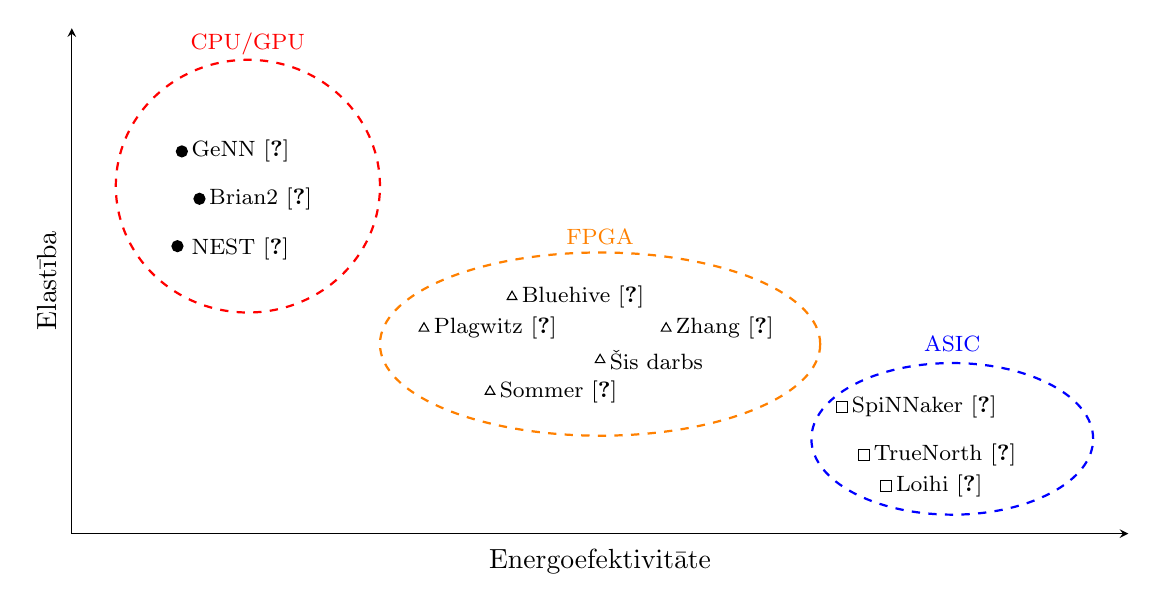
\begin{tikzpicture}
\def\Cx{4.0}
\def\Cy{11.0}
\def\Fx{12.0}
\def\Fy{6.0}
\def\Ax{20.0}
\def\Ay{3.0}
\begin{axis}[
    xlabel={Energoefektivitāte},
    ylabel={Elastība},
    xmin=0, xmax=24,
    ymin=0, ymax=16,
    xtick=\empty,
    ytick=\empty,
    axis lines=left,
    width=15cm,
    height=8cm
]

\addplot[only marks, mark=*] coordinates {(2.4,9.1)};
\node[anchor=west] at (axis cs:2.5,9.0) {\footnotesize NEST \cite{gewaltig2007}};

\addplot[only marks, mark=*] coordinates {(2.9,10.6)};
\node[anchor=west] at (axis cs:2.9,10.6) {\footnotesize Brian2 \cite{stimberg2019}};

\addplot[only marks, mark=*] coordinates {(2.5,12.1)};
    \node[anchor=west] at (axis cs:2.5,12.1) {\footnotesize GeNN \cite{yavuz2016}};

\addplot[only marks, mark=triangle] coordinates {(\Fx-2.5,\Fy-1.5)};
\node[anchor=west] at (axis cs:\Fx-2.5,\Fy-1.5) {\footnotesize Sommer \cite{sommer2022}};

\addplot[only marks, mark=triangle] coordinates {(\Fx-4.0,\Fy+0.5)};
\node[anchor=west] at (axis cs:\Fx-4.0,\Fy+0.5) {\footnotesize Plagwitz \cite{plagwitz2025}};

\addplot[only marks, mark=triangle] coordinates {(\Fx-2.0,\Fy+1.5)};
\node[anchor=west] at (axis cs:\Fx-2.0,\Fy+1.5) {\footnotesize Bluehive \cite{moore2012}};

\addplot[only marks, mark=triangle] coordinates {(\Fx+1.5,\Fy+0.5)};
\node[anchor=west] at (axis cs:\Fx+1.5,\Fy+0.5) {\footnotesize Zhang \cite{zhang2024}};

\addplot[only marks, mark=triangle] coordinates {(\Fx,\Fy-0.5)};
\node[anchor=west] at (axis cs:\Fx,\Fy-0.5) {\footnotesize Šis darbs};

\addplot[only marks, mark=square] coordinates {(\Ax-2.5,\Ay+1.0)};
\node[anchor=west] at (axis cs:\Ax-2.5,\Ay+1.0) {\footnotesize SpiNNaker \cite{furber2014}};

\addplot[only marks, mark=square] coordinates {(\Ax-2.0,\Ay-0.5)};
\node[anchor=west] at (axis cs:\Ax-2.0,\Ay-0.5) {\footnotesize TrueNorth \cite{akopyan2015}};

\addplot[only marks, mark=square] coordinates {(\Ax-1.5,\Ay-1.5)};
\node[anchor=west] at (axis cs:\Ax-1.5,\Ay-1.5) {\footnotesize Loihi \cite{orchard2021}};

\draw[blue, dashed, thick]
    (axis cs:\Ax,\Ay) ellipse (3.2 and 2.4);

\node[blue] at (axis cs:\Ax,6.0) {\footnotesize ASIC};

\draw[orange, dashed, thick]
    (axis cs:\Fx,\Fy) ellipse (5.0 and 2.9);

\node[orange] at (axis cs:\Fx,\Fy+3.4) {\footnotesize FPGA};

\draw[red, dashed, thick]
    (axis cs:\Cx,\Cy) ellipse (3.0 and 4.0);

\node[red] at (axis cs:\Cx,\Cy+4.5) {\footnotesize CPU/GPU};

\end{axis}
\end{tikzpicture}
\caption{Kompromiss starp energoefektivitāti un elastību dažādās SNN simulācijas un aparatūras platformās.}
\label{fig:hw_tradeoff}
\end{figure}

Šī pētījuma vispārējais mērķis ir izstrādāt un novērtēt pārkonfigurējamas, uz \Gls{fpga} balstītas impulsu neironu tīklu
paātrināšanas metodes, kas nodrošina mazas jaudas un zema latentuma inferenci attēlu klasifikācijai un objektu detektēšanai,
vienlaikus risinot dziļo impulsu neironu tīklu atmiņas mērogojamības ierobežojumus.

Šī mērķa sasniegšanai izvirzīti šādi pētnieciskie uzdevumi:
\begin{enumerate}
\item Izpētīt konvolucionālo impulsu neironu tīklu realizāciju aparatūrā un tās ierobežojumus, piemēram, svaru
  kvantēšanas ietekmi uz klasifikācijas veiktspēju, un noteikt \Gls{fpga} realizācijai piemērotu arhitektūru un skaitlisko
    precizitāti.

\item Izstrādāt un realizēt pārkonfigurējamu \Gls{fpga} paātrinātāju konvolucionālajiem impulsu neironu tīkliem, kas atbalsta
  dažādas tīklu konfigurācijas un impulsu neironu modeļus.

\item Izstrādāt un novērtēt atmiņas arhitektūru dziļāku tīklu atbalstam, apvienojot svaru glabāšanu mikroshēmā ar membrānas
  potenciālu straumēšanu ārpus mikroshēmas, lai samazinātu mikroshēmas iekšējās atmiņas prasības.

\item Izpētīt impulsu neironu tīklu piemērotību 3D objektu detektēšanai, izmantojot LiDAR un lidojuma laika punktu mākoņu
  reprezentācijas, tostarp novērtēt detektēšanas veiktspēju ar dažādām sensoru modalitātēm un iespējamās energoefektivitātes
    priekšrocības.

\item Eksperimentāli novērtēt \Gls{fpga} inferences latentumu, aparatūras resursu izmantojumu un jaudas patēriņu, kā arī
  izvērtēt piedāvāto impulsu neironu tīklu modeļu energoefektivitāti salīdzinājumā ar tradicionālajiem mākslīgajiem neironu
    tīkliem.

\end{enumerate}

Pētījuma mērķa un uzdevumu izpilde tiek novērtēta ar šādām trim tēzēm, kas attiecas uz aparatūras paātrināšanu un \Gls{snn}
arhitektūrāmu telpiski temporālu datu apstrādei:
\begin{itemize}

\item \textbf{1. tēze:} Impulsu neironu tīkls, kas realizēts pārkonfigurējamā \Gls{fpga} paātrinātājā un izmanto kvantētus
  svarus ar mazu bitu skaitu, saglabā klasifikācijas veiktspējas atšķirību 5~\% robežās no ekvivalenta pilnas precizitātes
    \Gls{snn} modeļa \textit{MNIST} un \textit{Caltech-101} veiktspējas testos, vienlaikus nodrošinot izmērīto dinamisko jaudas
    patēriņu zem 0,5~W un saglabājot elastību dažādām tīklu konfigurācijām un impulsu neironu modeļiem.

\item \textbf{2. tēze:} \Gls{snn} ir piemērojami 3D objektu detektēšanas uzdevumiem punktu mākoņu reprezentācijās, sasniedzot
  vismaz 70~\% vidējo precizitāti autonomās braukšanas transportlīdzekļu detektēšanas veiktspējas testā un vienlaikus nodrošinot
    analītiski novērtētu inferences enerģijas samazinājumu vismaz par 25~\% salīdzinājumā ar ekvivalentiem 3D objektu
    detektēšanas \Gls{ann} modeļiem.

\item \textbf{3. tēze:} Pārkonfigurējama konveijerizēta \Gls{fpga} arhitektūra, kas apvieno svaru glabāšanu mikroshēmā ar
  membrānas potenciālu straumēšanu ārpus tās, samazina iekšējās atmiņas prasības vismaz par 50~\%
    neiromorfajā \textit{Caltech-101} attēlu klasifikācijas veiktspējas testā, vienlaikus saglabājot inferences latentumu zem
    10~ms.

\end{itemize}

Šī promocijas darba galvenais ieguldījums ir divi savstarpēji papildinoši risinājumi: pārkonfigurējama, uz \Gls{fpga}
balstīta \Gls{snn} paātrinātāja izstrāde un impulsu konvolūcijas arhitektūra 3D-SCNN objektu detektēšanai punktu mākoņos.

Pirmais ieguldījums ir konfigurējams, uz PCIe balstīts \Gls{fpga} paātrinātājs, kas atbalsta dažādas konvolucionālo tīklu
konfigurācijas un impulsu neironu modeļus bez atkārtotas aparatūras sintēzes. PCIe ļauj paātrinātāju integrēt esošajos
datorredzes ietvaros, nodrošinot elastīgu eksperimentālu platformu dažādu \Gls{snn} arhitektūru un aparatūras konfigurāciju
novērtēšanai. Šī pieeja novērtēta attēlu klasifikācijas uzdevumos, demonstrējot, ka svaru kvantēšana un realizācija
aparatūrā saglabā novērtēto tīklu klasifikācijas veiktspēju. Paātrinātāja arhitektūrā izmantota mikroshēmas iekšējās un
ārējās atmiņas shēma, lai samazinātu iekšējās atmiņas apjomu un uzlabotu mērogojamību, saglabājot zemu inferences latentumu.

Otrs nozīmīgais ieguldījums ir 3D-SCNN arhitektūras izstrāde objektu detektēšanai, izmantojot laikā kodētus LiDAR un
\Gls{tof} punktu mākoņu datus. Pētījums ir vērsts uz 3D objektu detektēšanu, jo tā ir būtiska vides uztveres sastāvdaļa
autonomajās sistēmās, piemēram, autonomajos transportlīdzekļos un mobilajos robotos, kas darbojas ar ierobežotu enerģijas
budžetu. Šāda informācija ir svarīga šķēršļu apiešanai un ceļa plānošanai drošas navigācijas nodrošināšanai. Piedāvātā
3D-SCNN arhitektūra pēta \Gls{snn} piemērotību šim uzdevumam. Piedāvātajā arhitektūrā impulsu konvolūcijas pazīmju iegūšana
apvienota ar detektēšanas galvām, lai prognozētu orientētus robežu taisnstūrus. Tās veiktspēja novērtēta ar
\textit{KITTI} datu kopu un iegūtajiem \Gls{tof} datiem, demonstrējot piemērotību praktiskiem datorredzes uzdevumiem. Turklāt
analītiski enerģijas salīdzinājumi norādīja uz iespēju samazināt aprēķinu enerģiju salīdzinājumā ar ekvivalentām tradicionālo
\Gls{ann} arhitektūrām.

Šis ieguldījums uzlabo pārkonfigurējamas aparatūras arhitektūras impulsu skaitļošanai un nodrošina pamatu impulsu modeļu
turpmākai ieviešanai energoefektīvā pārkonfigurējamā aparatūrā.

Promocijas darbs ir tiešs rezultāts pētījumiem par uz \Gls{fpga} balstītiem paātrinātājiem, \Gls{snn} un neiromorfajām
tehnoloģijām, kas veikti Elektronikas un datorzinātņu institūtā (EDI), Latvijā, šādu pētniecības projektu ietvaros:
\begin{itemize}
\item \textit{Horizon 2020 ECSEL JU} „Advanced packaging for photonics, optics and electronics for low-cost manufacturing in Europe” (APPLAUSE, GA:826588)\footnote{https://applause-ecsel.eu/};
\item \textit{Horizon 2020 ECSEL JU} „Automotive Intelligence for/at Connected Shared Mobility” (AI4CSM, GA:101007326)\footnote{https://ai4csm.eu/};
\item \textit{Horizon Europe Chips JU} „Intelligent, Safe and Secure Connected Electrical Mobility Solutions: Towards European Green Deal and Seamless Mobility” (EcoMobility, GA 101112306)\footnote{https://www.ecomobility-project.eu/};
\item \textit{Horizon Europe Chips JU} „Ensuring European ECS Value Chain Sovereignty through Shaping the Future of ECS for Automotive Applications” (ShapeFuture, GA:101139996)\footnote{https://shapefuture.eu/}.
\end{itemize}

Pārējā promocijas darba struktūra ir šāda. 2. nodaļā sniegts teorētiskais pamatojums, sākot ar neiromorfās skaitļošanas un
galveno impulsu neironu modeļu pārskatu, kam seko impulsu kodēšanas metodes, impulsu neironu tīklu arhitektūras un apmācības
metodes. Tajā aplūkota arī uz \Gls{fpga} balstīta neiromorfā skaitļošana, tostarp mūsdienu \Gls{fpga} arhitektūras, neironu
modeļu realizācijas un saistītās aparatūras sistēmas. 3. nodaļā detalizēti aprakstīta realizācijas metodoloģija, izskaidrojot uz
PCIe balstīta \Gls{fpga} paātrinātāja izstrādi pārkonfigurējamiem konvolucionāliem impulsu neironu tīkliem, kā arī telpiski
temporālu objektu detektēšanas ietvaru, kas izmanto lidojuma laika datus, īpašu uzmanību pievēršot kodēšanai, konvolūcijas
apstrādei un neironu realizācijai. 4. nodaļā sniegti eksperimentālie rezultāti, tostarp veiktspējas novērtēšanas metrikas un
piedāvāto sistēmu salīdzinošā analīze. Darba noslēgumā apkopoti galvenie secinājumi, ieguldījums un ieteikumi turpmākajiem
pētījumiem.




\section{Teorētiskais pamatojums}
  \subsection{Neiromorfā skaitļošana} % 1.1

    \subsubsection{Impulsu neironu modeļi} % 1.1.1
      \paragraph{Integrējošā neirona modelis ar noplūdi}\mbox{} \\
      Lai gan detalizēti modeļi ļauj ģenerēt signālus, kas cieši līdzinās īstu neironu signāliem, šādu neironu tīklu realizācija un analīze ir sarežģīta to kompleksās uzvedības dēļ. Lai atvieglotu impulsu kodēšanas un izplatīšanās izpēti neironu tīklos, izstrādāti formāli impulsu ģenerēšanas modeļi. Vēsturiski visplašāk izmantotie formālie modeļi ir Lapika \cite{abbott1999} un Steina \cite{stein1967} izstrādātie \Gls{if} un \Gls{lif} modeļi. Abus modeļus bieži realizē aparatūrā.

Lapika modelētais \Gls{if} neirons sastāv no elektriskās ķēdes ar kondensatoru, kas reprezentē membrānas kapacitāti un uzkrāj ieejas strāvu, līdz tiek sasniegts impulsu ģenerēšanas slieksnis. \Gls{lif} modelis to paplašina, pievienojot paralēli membrānas kapacitātei pieslēgtu membrānas noplūdes rezistoru, izveidojot \ref{fig:lif_circuit}. attēlā parādīto ekvivalento RC ķēdi. Kad membrānas potenciāls sasniedz noteiktu slieksni, tiek ģenerēts darbības potenciāls un kondensators izlādējas. Lai gan dažādu membrānas vadītspēju ietekme netiek ņemta vērā, daudziem mērķiem pietiek ar vienkāršo \Gls{if} modeli.

\begin{figure}[hb]
  \centering
  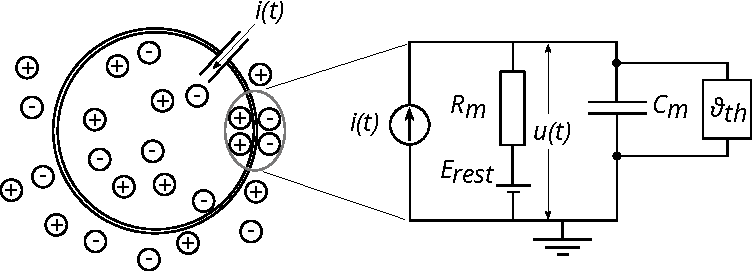
\includegraphics[width=1.0\linewidth]{fig/lif_circuit_membrane.pdf}
  \caption{Integrējošā impulsu neirona modelis ar noplūdi. Šūnas membrāna saņem ieejas strāvu $i(t)$, kas palielina membrānas lādiņu.}
  \label{fig:lif_circuit}
\end{figure}

\Gls{lif} modelī strāva \(i(t)\) uzlādē RC ķēdi, līdz spriegums uz kondensatora \(C_m\) sasniedz noteiktu sliekšņa vērtību \(\vartheta_{th}\). Šajā ķēdē strāva \(i(t)\) sadalās strāvā \(i_C\), kas plūst caur kondensatoru, un strāvā \(i_R\), kas raksturo viena membrānas kanāla pretestību \cite{kim2020}:
\begin{equation}
    i(t) = i_R + i_C = \frac{u(t) - E_{rest}}{R_m} + C_m\frac{du}{dt},
    \label{eq:LIF_current}
\end{equation}
kur \(C_m\) apzīmē membrānas kapacitāti un \(R_m\) ir vienkāršotā kanāla pretestība. Apzīmējot membrānas laika konstanti ar \(\tau_m = R_mC_m\), no (\ref{eq:LIF_current}) iegūst laikā mainīgo membrānas potenciālu, ko rada impulsu strāvas \(i(t)\), kuras caur sinaptiskajiem savienojumiem saņemtas no citiem neironiem:
\begin{equation}
    \tau_m \frac{du}{dt} = - (u(t) - E_{rest}) + R_mi(t),
    \label{eq:LIF_model}
\end{equation}
kur \(i(t)\) ir no atsevišķām sinapsēm saņemto individuālo sinaptisko strāvu summa, katru reizinot ar atbilstošo sinaptiskā svara koeficientu:
\begin{equation}
    i(t) = \sum_{j=1}^{N_{pre}} w_{j}i_j(t),
\end{equation}
kur \(N_{pre}\) ir presinaptisko neironu skaits. Modelis vienkāršojas līdz \Gls{if} neironam, ja membrānas pretestībai piešķir lielu vērtību \(R_m \to \infty\).

Kad membrānas potenciāls sasniedz impulsu ģenerēšanas slieksni, \Gls{lif} neirons izstaro impulsu un pārraida to nākamajiem neironiem. Neirona izejas signāls ir Diraka delta funkcijas impulss \(\delta(t - t^f)\), kur laiku \(t^f\) iegūst, salīdzinot membrānas potenciālu \(u(t^f)\) ar sliekšņa vērtību \(\vartheta_{th}\):
\begin{equation}
    t^f: u(t^f) = \vartheta_{th}
\end{equation}
Matemātiski šādu impulsu notikumu virkni var aprakstīt šādi \cite{kim2020}:
\begin{equation}
    s(t) = \sum_f \delta(t - t^f)
\end{equation}

Impulsa brīdī potenciāls atgriežas nullē vai miera stāvoklī \(E_{rest}\), kas kalpo par sākuma nosacījumu nākamajai aprēķinu iterācijai. Alternatīvi membrānas potenciālu var samazināt par impulsu ģenerēšanas slieksni \(\vartheta_{th}\), veicot mīksto atiestatīšanu, kas precīzāk atdarina \Gls{relu} funkciju \cite{hwang2024, park2019}.

Ja sinaptiskā strāva ir nulle \(i(t) = 0\), membrānas potenciāla vienādojums (\ref{eq:LIF_model}) vienkāršojas līdz
\begin{equation}
    \tau_m \frac{du}{dt} = - (u(t) - E_{rest}).
\end{equation}
Analītiskais atrisinājums ir
\begin{equation}
    u(t) = E_{rest} + (u(t_0) - E_{rest}) \exp \left ( - \frac{t - t_0}{\tau_m} \right ).
    \label{eq:LIF_exp}
\end{equation}
Tas parāda, ka membrānas potenciāls eksponenciāli samazinās līdz miera potenciālam \(E_{rest}\) ar laika konstanti \(\tau_m\).

Vienādojums (\ref{eq:LIF_exp}) apraksta precīzu membrānas potenciālu nepārtrauktā laikā. Tomēr digitālā aparatūra veic diskrēta laika atjaunināšanu, nevis risina nepārtrauktus diferenciālvienādojumus. Diskrēta laika \Gls{snn} simulācijās eksponenciālās dilšanas tiešai novērtēšanai katrā laika solī būtu jāaprēķina:
\begin{equation}
    \exp \left ( \frac{-\Delta t}{\tau_m} \right ).
\end{equation}
Liela mēroga \Gls{snn} ar miljoniem neironu un daudziem laika soļiem tas rada lielu skaitļošanas sarežģītību. Tā kā eksponenciālās operācijas nav izdevīgas digitālo shēmu realizācijās, parasti priekšroku dod aproksimācijai ar bitu nobīdes operācijām vai skaitliskiem atrisinājumiem \cite{corradi2021}. Lielākā daļa \Gls{snn} aparatūras realizāciju diferenciālvienādojumu aproksimē ar vienkāršām skaitliskās integrēšanas metodēm, piemēram, tiešo Eilera metodi, kas eksponenciālās funkcijas aprēķinu aizstāj ar rekurentu vienādojumu.

\ref{fig:lif_simulation}. attēlā parādīta skaitliski atrisināta \Gls{if} modeļa simulācija, tam pievadot konstantas strāvas pakāpienu. Pēc stimula pievadīšanas \(u(t)\) pieaug sliekšņa \(\vartheta_{th}\) virzienā saskaņā ar (\ref{eq:LIF_current}) un, to sasniedzot, izstaro impulsu. Šī vienkāršā uzvedība bez kanālu vadītspējas ilustrē, kādēļ \Gls{if} modelis ir skaitļošanas ziņā izdevīgs, pat neietverot Hodžkina–Hakslija modeļa detalizēto kanālu dinamiku.
\begin{figure}[!t]
\centering
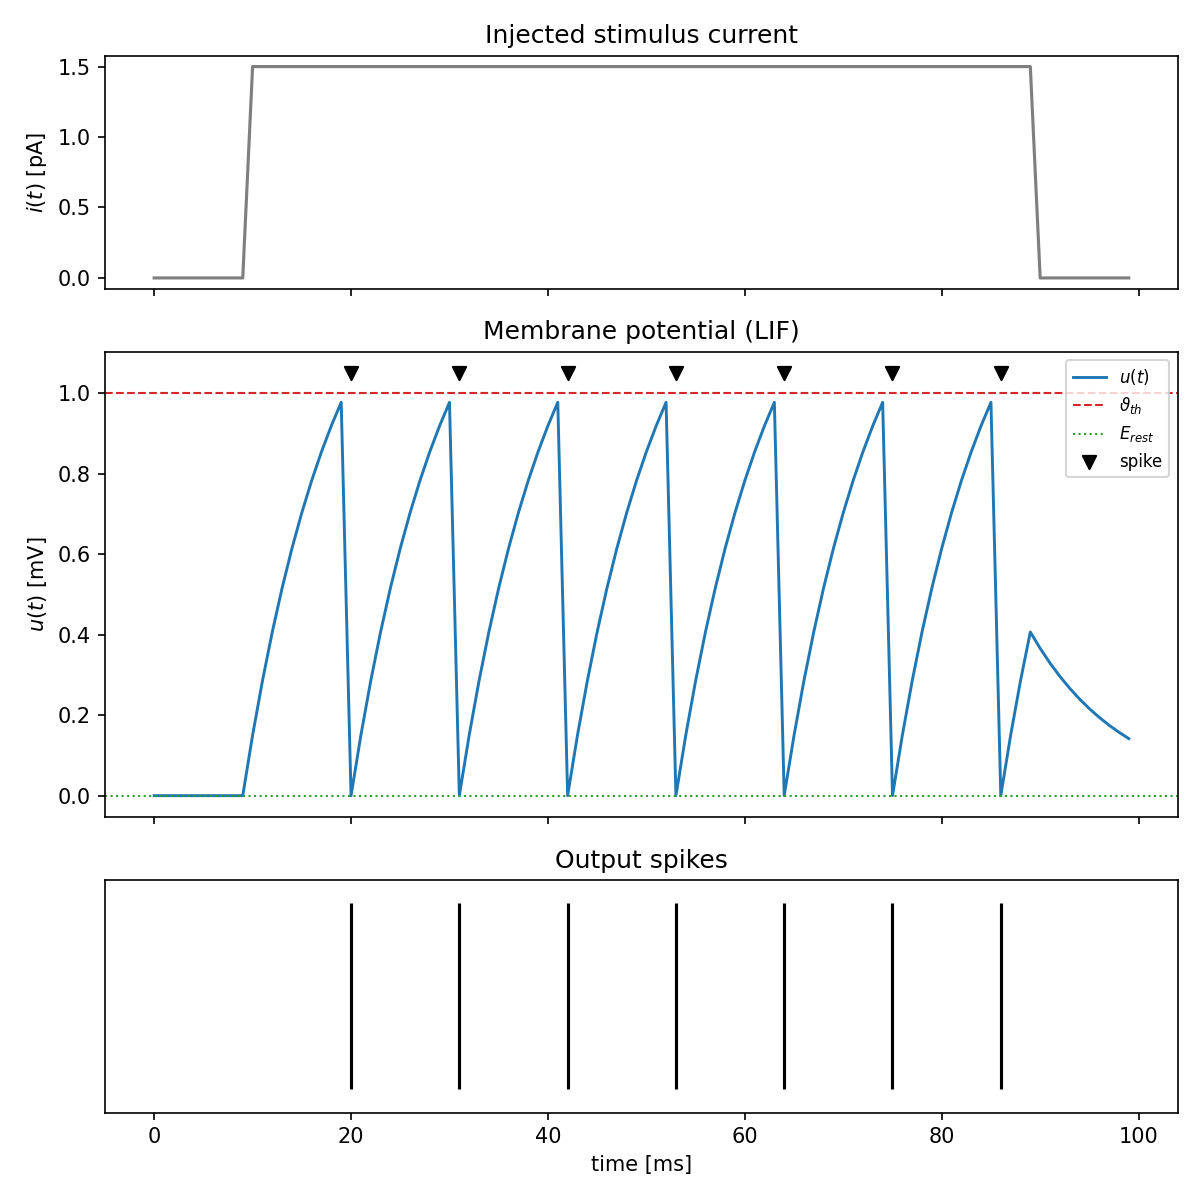
\includegraphics[width=\linewidth]{fig/lif_simulation.png}
\caption{LIF neirona simulētā reakcija uz strāvas pakāpienu.}
\label{fig:lif_simulation}
% \par\smallskip
% {\footnotesize \textit{Injected stimulus current} — pievadītā stimulējošā strāva; \textit{Membrane potential (LIF)}
%   — membrānas potenciāls (LIF); \textit{Output spikes} — izejas impulsi; \textit{spike} — impulss; \textit{time}
%   — laiks.\par}
\end{figure}

Turklāt ir piedāvātas vairākas precizitātes uzlabošanas metodes \Gls{lif} neirona līmenī, lai atvieglotu apmācību un mazinātu
precizitātes zudumu \cite{Fang2021, wang2022, guo2022}. Tiešās izplatīšanas laikā sliekšņa operācija, kas kvantē membrānas
potenciālu līdz 0 vai 1, neizbēgami rada informācijas zudumu. Efektīvs veids, kā mazināt šī vienkāršā modeļa radīto zudumu,
ir padarīt dažus ar membrānu saistītos hiperparametrus apmācāmus. Nesen darbā \cite{Fang2021} parādīts, ka \Gls{snn} ar
parametriskiem \Gls{lif} neironiem pārspēj modernākās metodes gan statiskajās, gan neiromorfajās datu kopās. Papildus sinapšu
svariem par apmācāmu parametru izmantota membrānas laika konstante. Citos darbos \Gls{snn} mācīšanās spēju uzlabošanai
izmantots impulsu neirons ar adaptīvu slieksni \cite{wang2022}. Darbā \cite{guo2022} sniegts visaptverošs pārskats par
dažādām parametriskām, neirona līmeņa apmācības metodēm.



      \paragraph{Ižikeviča modelis}\mbox{} \\
      Savstarpēji savienoti \Gls{lif} neironi digitālā arhitektūrā ir plaši izmantota izvēle liela mēroga \Gls{snn} ar efektīvu
resursu patēriņu, tomēr sarežģītākas impulsu ģenerēšanas dinamikas izpētei sistēmai nepieciešams augstāks bioloģiskās
līdzības līmenis. Lai precīzāk atdarinātu neirona uzvedību, parasti izvēlas reālistiskākus modeļus, kas spēj radīt dažādus
pulsēšanas režīmus, piemēram, Ižikeviča modeli \cite{Izhikevich2003}, taču tas palielina skaitļošanas sarežģītību.

Ižikeviča neirona modelī \cite{Izhikevich2003} Hodžkina–Hakslija neirona modelis \cite{hodgkin1952} reducēts līdz šādai
parasto diferenciālvienādojumu sistēmai:
\begin{equation}
\begin{cases}
  \label{eq:izhi}
  v' = 0{,}04v^{2} + 5v + 140 - u + I \\
  u' = a(bv - u),
\end{cases}
\end{equation}
kur \(v\) apzīmē membrānas potenciālu, \(u\) ir membrānas atjaunošanās mainīgais, \(a\) nosaka atjaunošanās mainīgā laika
mērogu un \(b\) raksturo jutību pret zemsliekšņa svārstībām.

Kad impulss sasniedz potenciāla slieksni, sistēma tiek atiestatīta uz pēcimpulsa stāvokli:
\begin{equation}
  \label{eq:postspike}
  v \geq V_{th} \text{, tad } \{v = c, u = u + d\},
\end{equation}
kur parametri \(c\) un \(d\) raksturo membrānas potenciāla un atjaunošanās mainīgā pēcimpulsa atiestatīšanas vērtības.
Pretstatā bioloģiski nereālistiski vienkāršajam \Gls{lif} modelim šis modelis spēj atveidot smadzeņu garozas neironiem raksturīgo atsevišķu
impulsu un impulsu kopu dinamiku.




    \subsubsection{Impulsu neironu tīkla arhitektūra} % 1.1.3
      \paragraph{Konvolūcijas slāņi}\mbox{} \\
      Konvolūcijas slāņi ģenerē pazīmju kartes, iegūstot vizuālas pazīmes, kas līdzinās orientētu malu detektoriem un Gabora filtru
izejām \cite{tavanaei2019}. Konvolūcijas slāņus plaši izmanto \Gls{snn} arhitektūrās, parasti aizstājot \Gls{relu}
aktivācijas ar \Gls{if} vai \Gls{lif} neironiem \cite{cao2015}. Šādi tīkli objektu detektēšanā notikumu attēlu datu kopās
pārspēj tradicionālos \Gls{ann} \cite{zhang2023}. Ir izveidoti \Gls{snn}, kuru pamatā ir esošas \Gls{cnn} arhitektūras,
piemēram, \textit{VGG} \cite{na2022}. Dziļākie slāņi efektīvi apvieno iepriekšējo slāņu pazīmes, lai iegūtu arvien
sarežģītākas pazīmes. Ieejas pazīmju karte tiek sadalīta mazākās neironu apakškopās. Katrs nākamā slāņa neirons saņem
impulsus no savas neironu apakškopas un tie tiek reizināti ar svaru kodolu \cite{tavanaei2017}:
\begin{equation}
  x^{t,l}_{i,j} = \sum^{K}_{m=0} \sum^{K}_{n=0} w^l_{m,n} s^{t,l-1}_{i+m,j+n}
  \label{eq:lif_conv}
\end{equation}
\begin{equation}
  {u}^{t,l}_{i,j} = u^{t-1,l}_{i,j}(1 - s^{t,l}_{i,j}) + x^{t,l}_{i,j}
  \label{eq:lif_v}
\end{equation}
\begin{equation}
  s^{t,l}_{i,j} = \Theta ({u}^{t,l}_{i,j} - \vartheta_{th}),
  \label{eq:lif_spike}
\end{equation}
kur \(w^l_{m,n}\) ir svaru kodols, kas ir kopīgs visam \(l\)-tajam slānim, lai samazinātu parametru skaitu līdzīgi kā tradicionālajos \Gls{cnn}, pieņemot, ka vienā pozīcijā noderīga kodola pazīme ir noderīga arī citās telpiskās pozīcijās. \(K^2\) ir ieejas pazīmju kartes kodola neironu skaits, ko izmanto \(i\)-tā neirona ieejas strāvas \(x^{t,l}_{i,j}\) ģenerēšanai, un \(s^{t,l-1}_{i+m,j+n}\) ir impulsi no \(i\)-tā ieejas kodola laika solī \(t+1\).

Tomēr praktiskos gadījumos ieejas tenzoriem ir vairāki ieejas kanāli \(C_{in}\) (piemēram, RGB krāsu kanāli vai pazīmju karšu kanāli). Tad katrs no \(C_{out}\) izejas kanāliem \(c\) tiek iegūts, veicot ieejas konvolūciju ar atsevišķu 3D kodolu, kura izmērs ir \(C_{in} \times K \times K\), un sinaptisko strāvu telpiskajā pozīcijā \(i,j\) katrā izejas kanālā nosaka
\begin{equation}
    x^{t,l}_{c,i,j} = \sum^{C_{in}}_{d=0} \sum^{K}_{m=0} \sum^{K}_{n=0} w^l_{c,d,m,n} s^{t,l-1}_{d,i+m,j+n},
    \label{eq:channel_conv}
\end{equation}
kur \(d\) indeksē ieejas kanālus, \(c\) indeksē izejas kanālus un \(w^l_{c,d,m,n}\) ir koplietotie konvolūcijas svari slānī \(l\). Līdzīgi katram izejas kanālam tiek ģenerēts membrānas potenciāls \({u}^{t,l}_{c,i,j}\) un impulsi \(s^{t,l}_{c,i,j}\).

Šādi \((K \times K)\) kodolu kopu izmanto \((H \times W)\) pikseļu ieejas pazīmju kartes konvolūcijai, iegūstot izejas pazīmju kartes ar
\begin{equation}
  \left( \frac{H - K + 2p}{s} + 1 \right) \times \left( \frac{W - K + 2p}{s} + 1 \right)
\end{equation}
neironiem, kur \(p\) ir papildinājuma apjoms pie malām un \(s\) ir solis - pikseļu skaits, par kuru kodolu pārvieto vienā reizē.

\begin{figure}[h!]
\begin{adjustbox}{max width=\linewidth,center}
\centering
    \begin{tikzpicture}[
        >=Stealth,
        neuron/.style={circle, draw, fill=gray!50, minimum size=0.9cm},
        spike/.style={rectangle, draw, minimum width=1.2cm, minimum height=0.6cm},
        weight/.style={midway, fill=white, inner sep=1pt},
        kcell/.style={draw, minimum width=0.6cm, minimum height=0.6cm, font=\scriptsize, fill=orange!15},
    ]
    \draw[step=0.6cm, gray] (0,0) grid (4.2,4.2);
    \foreach \x in {1.2,1.8,2.4}{
        \foreach \y in {1.2,1.8,2.4}{
            \filldraw[fill=gray!30, draw=black] (\x,\y) rectangle ++(0.6,0.6);
        }
    }
    \foreach \i in {0,...,6}{
        \foreach \j in {0,...,6}{
            \pgfmathtruncatemacro{\spike}{rnd>0.75}
            \node at ({0.3+0.6*\i},{0.3+0.6*\j}) {\spike};
        }
    }
    \node[below=0.2cm] at (2.1,0) {\small Impulsu pazīmju karte $s^{t,l-1}$};
    \node[above=0.15cm] at (2.1,4.2) {\small $3 \times 3$ uztveres lauks};

    \foreach \r in {0,...,2} {
        \foreach \c in {0,...,2} {
            \pgfmathtruncatemacro{\rr}{\r+1}
            \pgfmathtruncatemacro{\cc}{\c+1}
            \node[kcell] (k-\r-\c) at ({6.4+0.8*\c},{2.1+0.6*(1-\r)}) {$w_{\rr\cc}$};
        }
    }
    \node[above=0.15cm] at (6.7,2.1+0.6+0.3) {\small Kodols $w^l_{m,n}$};

    \node at (5.15,2.1) {\Large $\circledast$};
    \draw[-] (3.0,1.8) -- (4.65,2.1);
    \draw[-] (3.0,2.4) -- (4.65,2.1);

    \node[neuron, right=1.4cm of k-1-2] (sum) {$\sum_{m,n}$};
    \draw[->] (k-0-2) -- (sum);
    \draw[->] (k-2-2) -- (sum);

    \node[neuron, right=1.8cm of sum] (spikef) {${u}^{t,l}_{i,j}$};
    \node[spike, right=1.8cm of spikef] (y) {$s^{t,l}_{i,j}$};
    \draw[->] (sum) -- (spikef);
    \draw[->] (spikef) -- node[weight] {$\Theta(\cdot)$} (y);

    \node[above=0.3cm] at (9.6,2.6) {\small Konvolūcija};
    \node[above=0.3cm of spikef] {\small Impulsu neirons};
    \end{tikzpicture}
\end{adjustbox}
\caption{Impulsu konvolūcijas slānis. Koplietots reālu vērtību $3 \times 3$ kodols $w^l_{m,n}$ tiek konvolvēts ar binārās ieejas impulsu pazīmju kartes $s^{t,l-1}$ uztveres lauku. Svērto summu integrē impulsu neirons, kas ģenerē izejas impulsu $s^{t,l}_{i,j}$ pozīcijā $(i,j)$.}
\label{fig:spiking_conv_receptive_field}
\end{figure}



  \subsection{Uz FPGA balstīta neiromorfā skaitļošana}
    \subsubsection{Uz FPGA balstīti neironu modeļi}
      \paragraph{Integrējošā neirona modelis ar noplūdi}\mbox{} \\
      \Gls{lif} neirona modelis un tā varianti ir plaši izmantoti neiromorfajās un digitālās aparatūras realizācijās to relatīvās
vienkāršības dēļ salīdzinājumā ar bioloģiski precīziem modeļiem \cite{sommer2022, corradi2021}. Piemēram, \Gls{lif} modelim vienā
laika solī nepieciešamas tikai 5 peldošā punkta operācijas, savukārt Hodžkina–Hakslija modelim nelineārās jonu kanālu
dinamikas dēļ vajag līdz pat 1200 operācijām \cite{hwang2024}. Tomēr shēmu izveide \Gls{lif} neironu simulācijai lielā mērogā
joprojām ir sarežģīta \cite{kousanakis2017}.

Kā parādīts (\ref{eq:LIF_exp}), \Gls{lif} membrānas dinamikas analītiskais atrisinājums ietver eksponenciālās dilšanas
locekli. Eksponenciālās funkcijas tieša aprēķināšana katrā laika solī katram neironam var kļūt skaitļošanas ziņā dārga, īpaši
\Gls{fpga} sistēmās.

Viena aparatūras risinājumu kategorija eksponenciālo funkciju aproksimē tieši. Bieži izmantotās pieejas ietver \gls{pwl}
aproksimācijas \cite{chakraborty2025}, bitu nobīdes metodes ar bāzi 2 \cite{corradi2021}, uz \gls{cordic} balstītas
realizācijas \cite{heidarpour2016} un uzmeklēšanas tabulu metodes \cite{kim2020}. Lai gan šīs pieejas ir efektīvas, tās
palielina sarežģītību un resursu patēriņu.

Otra risinājumu grupa analītiskās formas aprēķina vietā izmanto diferenciālvienādojuma skaitlisko diskretizāciju. Praksē
lielākā daļa \Gls{snn} apmācības un inferences rīku ķēžu izmanto šādus vienkāršotus diskrētus modeļus \cite{Fang2021},
demonstrējot augstas precizitātes inferences rezultātus. Dažās realizācijās \Gls{lif} dinamika tiek vēl vairāk vienkāršota, katrā laika solī samazinot membrānas potenciālu ar fiksētu dilšanas koeficientu \cite{gupta2020}.

Skaitlisko diskretizāciju iegūst, izmantojot tiešo Eilera metodi. Tad atvasinājumu aproksimē šādi \cite{guo2022, Fang2021}:
\begin{equation}
    \frac{du(t)}{dt} \approx \frac{u[t+1] - u[t]}{\Delta t}.
\end{equation}

To ievietojot nepārtraukta laika \Gls{lif} vienādojumā (\ref{eq:LIF_model}) \cite{guo2022, Fang2021}, iegūst
\begin{equation}
    \tau_m \frac{u[t+1] - u[t]}{\Delta t} = - u[t] + R_m i[t].
\end{equation}
Izsakot nākamo membrānas potenciālu, iegūst
\begin{equation}
    u[t+1] = u[t] + \frac{\Delta t}{\tau_m} \left(-u[t] + R_m i[t] \right).
\end{equation}
Pārkārtojot iegūst
\begin{equation}
    u[t+1] = \left(1 - \frac{\Delta t}{\tau_m}\right) u[t] + \frac{\Delta t}{\tau_m} R_m i[t].
\end{equation}
Dilšanas koeficientu var definēt kā
\begin{equation}
    \beta = 1 - \frac{\Delta t}{\tau_m},
\end{equation}
un atjaunināšanas izteiksme kļūst par
\begin{equation}
    u[t+1] = \beta u[t] + \frac{\Delta t}{\tau_m} R_m i[t].
    \label{eq:LIF_euler}
\end{equation}

Šis diskrētais atrisinājums novērš nepieciešamību aprēķināt eksponenciālo funkciju un reducē neirona atjaunināšanu līdz vienkāršām reizināšanas un saskaitīšanas operācijām. Digitālajā aparatūrā un GPU šādas operācijas ir ievērojami efektīvākas, tādēļ tiešā Eilera aproksimācija ir standarta izvēle lielu \Gls{snn} apmācībai un realizācijai aparatūrā. Turklāt aparatūras realizācijās dilšanas locekli $\beta u[t]$ var vienkāršot, lai izslēgtu reizinātājus. Ja dilšanas koeficientu ierobežo līdz daļai ar divnieka pakāpi,
\begin{equation}
    \beta = 1 - 2^{-k},
    \label{eq:quant_beta}
\end{equation}
membrānas atjaunināšanas izteiksmi
\begin{equation}
    u[t+1] = \beta u[t] + C_m i[t]
\end{equation}
var pārrakstīt šādi:
\begin{equation}
    u[t+1] = u[t] - \frac{u[t]}{2^k} + C_m i[t].
\end{equation}
Tā kā dalīšana ar $2^k$ fiksētā komata aritmētikā atbilst bitu nobīdei pa labi,
\begin{equation}
    u[t+1] = u[t] - (u[t] \gg k) + C_m i[t],
\end{equation}
dilšanas operāciju var realizēt, izmantojot tikai nobīdes un saskaitīšanas operācijas.



\section{Realizācijas metodoloģija} \label{sec:impl}
Šajā nodaļā izklāstīta promocijas darba pētījumos un to rezultātā tapušajās publikācijās izstrādātā realizācijas metodoloģija. Tā neapraksta tikai vienu sistēmu, bet apvieno vairāku publikāciju ieguldījumu kopīgā neiromorfās skaitļošanas ietvarā.

Darbs aptver realizācijas no impulsu neironu modeļiem līdz pilnīgai neiromorfās uztveres sistēmai. Vispirms pētītas bioloģiski iedvesmotu neironu modeļu aparatūras realizācijas. Tās izmantotas kā uz notikumiem balstītas apstrādes pamatelementi. Uz to pamata izstrādāts pārkonfigurējams \Gls{fpga} paātrinātājs konvolucionālo \Gls{snn} paātrināšanai aparatūrā. Visbeidzot izstrādāti dziļie konvolucionālie impulsu neironu tīkli praktiskiem uztveres uzdevumiem, izmantojot retinātus 3D sensoru datus.

Pārējā nodaļa sadalīta divās saistītās daļās. Pirmajā uzmanība pievērsta PCIe \Gls{fpga} paātrinātāja aparatūras arhitektūrai pārkonfigurējamu konvolucionālo \Gls{snn} paātrināšanai gan ar \Gls{lif}, gan Ižikeviča neironu modeļiem. Otrajā demonstrēta dziļo \Gls{snn} izmantošana 3D objektu detektēšanā ar LiDAR un lidojuma laika sensoriem, parādot modeļu un aparatūras risinājuma izmantošanu praktiskās autonomās uztveres sistēmās.

Realizācijas balstās uz promocijas darba izstrādes laikā publicētajiem pētījumiem. Ižikeviča neirona aparatūras realizācija pirmoreiz publicēta darbā \cite{lielamurs2023a}. Retināta impulsu objektu detektēšana ar LiDAR datiem balstās uz darbu \cite{lielamurs2024}, savukārt tās paplašinājums automobiļu \Gls{tof} sensoru sistēmai publicēts darbā \cite{lielamurs2025}. Visbeidzot pārkonfigurējamā \Gls{fpga} paātrinātāja arhitektūra ir darba \cite{lielamurs2026} galvenais ieguldījums.



\subsection{Uz PCIe balstīts FPGA paātrinātājs pārkonfigurējamiem konvolucionāliem impulsu neironu tīkliem} \label{sec:fpga_impl} % 3.1
  Šajā apakšnodaļā aprakstīta darbā \cite{lielamurs2026} piedāvātā \Gls{fpga} paātrinātāja arhitektūra, kas ir šajā promocijas
darbā aplūkotā pārkonfigurējamā konvolucionālā \Gls{snn} paātrinātāja galvenā realizācija. Piedāvātais risinājums paplašina
straumēšanas \Gls{fpga} paātrinātāju ietvaru uz PCIe balstītu aparatūras paātrinātāju izveidei ar specializētiem apstrādes
elementiem uz notikumiem balstītai skaitļošanai.

  \subsubsection{Paātrinātāja sistēmas vispārējā koncepcija} % 3.1.1
  

Paātrinātāja sistēmas pamatā ir \Gls{fpga} ietvars, kas paredzēts IP kodolu savienošanas un programmatūras integrācijas
atvieglošanai, īpaši uz PCIe balstītās \Gls{fpga} ierīcēs. Tā kā pats straumēšanas konveijeru izveides ietvars 
promocijas darba netiek pilnībā apskatīts, šeit apkopotas tikai piedāvāto neiromorfo paplašinājumu izpratnei nepieciešamās koncepcijas.

Ietvars, kas parādīts \ref{fig:overall_arch}. attēlā, ietver sistēmas arhitektūras komponentu VHDL bibliotēku, kodola telpas
draiveri un lietotāja telpas API. Tas izveido konveijerizētu paātrinātāju, savienojot konveijerizētas \Gls{pu} ar AXI-Stream.
Lietotājam jānorāda tikai IP kodolu nosaukumu un parametru saraksts. Ietvars arī nodrošina reģistru kartēšanu, ļaujot
komponentus konfigurēt no draivera.

Datu pārsūtīšanai starp resursdatora skaitļošanas platformu, SDRAM un paātrinātāju izmanto AXI4-Full DMA moduļus. Lietotāja telpas API atbalsta modeļa ielādi paātrinātājā un atvieglo inferences izpildi.

\begin{figure}[!t]
  \centering
  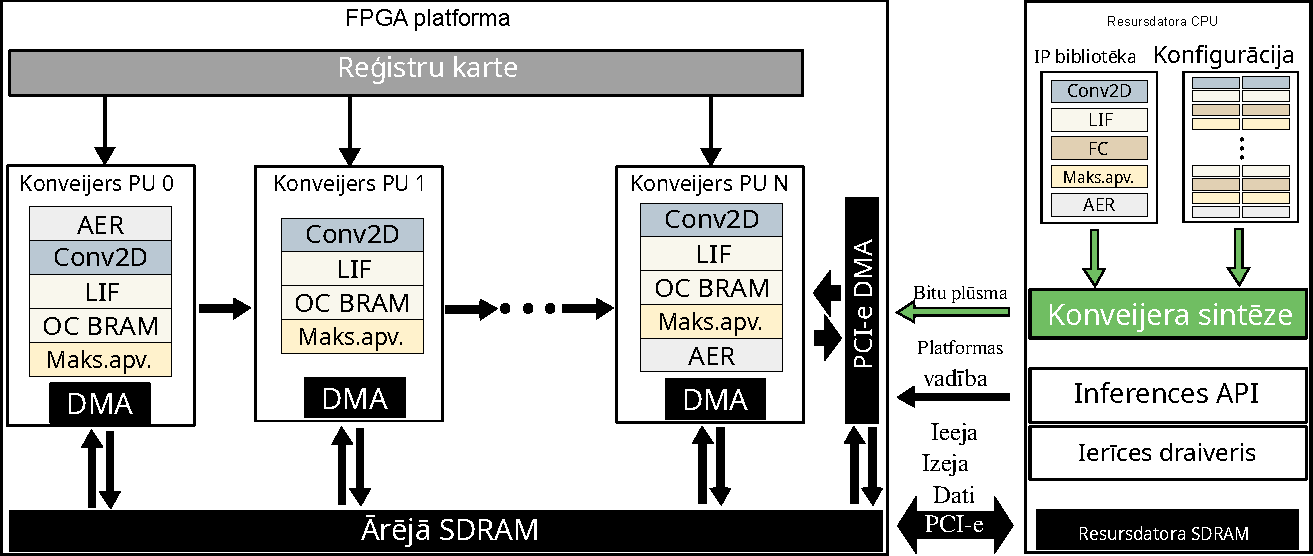
\includegraphics[width=0.75\linewidth]{fig/lv/snn_silhouse-v5.pdf}
  \caption{Automatizēta SNN paātrinātāja izveide heterogēnām skaitļošanas platformām.}
  \label{fig:overall_arch}
\end{figure}

Ietvars ir piemērots heterogēnām paātrinātāju sistēmām, kas CPU operācijām izmanto resursdatora skaitļošanas platformu un realizē \Gls{snn} inferenci PCIe \Gls{fpga} paplašināšanas kartēs. Tādēļ šajā darbā ietvars papildināts ar uz notikumiem balstītiem konvolūcijas, neironu, apvienošanas un impulsu kodēšanas apstrādes blokiem konveijerizētu neiromorfo sistēmu izveidei.

Turpmākajās sadaļās detalizēti aprakstīta katra \Gls{pu}.



  \subsubsection{Impulsu kodēšanas realizācija}
  

\Gls{snn} ieejas dati jākodē kā retu impulsu virknes, lai tie atbilstu impulsu neironu darbībai laikā. Tā vietā, lai
katrā laika solī pārraidītu visu neironu stāvokļus, tiek pārraidīti tikai neironi, kas ģenerē impulsu. Tas būtiski
samazina pārsūtāmo datu apjomu, ja impulsu aktivitāte ir reta. Vairumā gadījumu izmanto saspiestu \Gls{aer} reprezentāciju
\cite{sommer2022, plagwitz2025}, kas efektīvi kodē impulsu aktivitāti kā diskrētas notikumu adreses telpā un laikā.

Kā ilustrēts \ref{fig:aer_comm}. attēlā, kad neirons ģenerē impulsu, tā telpiskā pozīcija tiek kodēta adresē un pārraidīta pa sakaru kanālu. Uztvērējā adrese tiek dekodēta, lai atjaunotu impulsa notikumu. Tā kā impulsus ģenerē tikai aktīvie neironi, sakaru joslas platums mainās atkarībā no impulsu skaita, nevis neironu skaita \cite{purohit2022}.

\begin{figure}[!t]
  \centering
  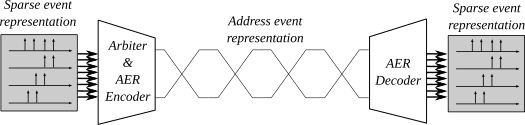
\includegraphics[width=0.8\linewidth]{fig/aer_encoder_decoder.png}
  \caption{AER saziņa.}
  \label{fig:aer_comm}
% \par\smallskip
% {\footnotesize \textit{Sparse event representation} — retināta notikumu reprezentācija; \textit{Arbiter \& AER Encoder} — arbitrs un AER kodētājs; \textit{Address event representation} — adrešu un notikumu reprezentācija; \textit{AER Decoder} — AER dekodētājs.\par}
\end{figure}

Šajā darbā tradicionālais \Gls{aer} protokols ir paplašināts, lai reprezentētu konvolucionālo \Gls{snn} slāņu radītās daudzkanālu pazīmju kartes. Saskaņā ar šo kodēšanas shēmu katru impulsu attēlo viena vesela skaitļa adrese, kas veidota, bitu līmenī savienojot telpiskos un kanāla indeksus, kā parādīts \ref{fig:aer_bits}. attēlā. Precīzāk, katra impulsa adrese \(a\) tiek kodēta kā bitu lauks:
\begin{equation}
    a[t] = (x \ll (b_h + b_c + 1)) | (y \ll (b_c + 1)) | (c \ll 1) | l,
\end{equation}
kur \(x, y\) ir 2D telpiskās koordinātas, \(c\) ir kanāla adrese un \(b_h, b_c\) ir iepriekš noteikts bitu skaits atkarībā no telpiskajām un kanālu dimensijām. Papildus \(l\) ir neobligāts jaunākās kārtas bits, ko izmanto atkārtotu vai vairāklīmeņu notikumu atšķiršanai vienā pozīcijā, ja nepieciešama reprezentācija ar vairāk nekā vienu aktīvu impulsa bitu.

\begin{figure}[!t]
  \centering
  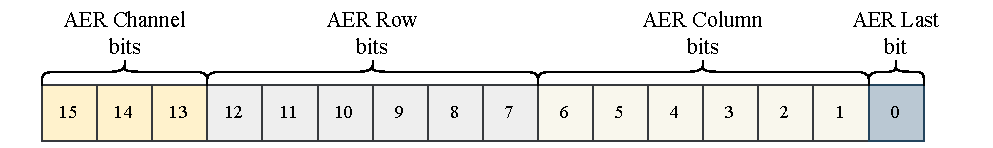
\includegraphics[width=0.8\linewidth]{fig/aer_bits.pdf}
  \caption{AER bitu lauks. Telpisko un kanāla indeksu savienošana bitu līmenī.}
  \label{fig:aer_bits}
\end{figure}

\(x, y\) vērtības nosaka, palielinot rindu un kolonnu rādītājus, līdz tiek atrasti impulsi. Pēc tam, izmantojot prioritātes kodētāju, impulsus kodē kanāla \(c\) binārā reprezentācijā, kas atbilst nozīmīgākās aktivizētās līnijas indeksam. Pilnu \Gls{aer} vārdu veido, bitu līmenī savienojot telpiskos \(x, y\) un kanāla \(c\) indeksus.

Impulsu adreses reprezentācija nodrošina efektīvāku glabāšanu un saziņu, kodējot visu nepieciešamo informāciju vienā vesela skaitļa vārdā. Kanāla indeksa reprezentācijai nepieciešamais bitu platums tiek efektīvi samazināts par \(\log_{2} N\), kur \(N\) ir vienā binārā impulsu vārdā kodēto kanālu skaits.


  \subsubsection{Uz notikumiem balstītas konvolūcijas realizācija}
  Laikā kodētos impulsu signālus no \Gls{aer} dekodētāja apstrādā uz notikumiem balstītu konvolūciju slāņi, kā ilustrēts \ref{fig:bsf_arch}.
attēlā. Šie slāņi atdarina sinaptiskās operācijas fiksētā uztveres laukā, veicot ieejas impulsu svērto summēšanu, kā
aprakstīts (\ref{eq:channel_conv}). Tā kā impulsi ir bināri ($s \in \{0,1\}$), apstrādes kodols tradicionālās \Gls{mac}
operācijas starp datiem un svariem aizstāj ar svaru bināro maskēšanu, reducējot impulsa un svara reizināšanu līdz
\begin{equation}
  w \cdot s =
  \begin{cases}
    w, & s=1 \\
    0, & s=0
  \end{cases}
\end{equation}
Tas ļauj reizināšanas operāciju aizstāt ar nosacītu svara izvēli. Tai seko \Gls{acc}, kas realizēta ar \Gls{pta}. Būtiski, ka šīs \Gls{acc} operācijas vada notikumi un tās notiek tikai tad, ja ir impulsi, ievērojami samazinot liekus aprēķinus.

Šajā shēmā svaru un nobīžu parametri tiek glabāti divportu \Gls{ocm} blokos tuvu apstrādes loģikai. Šī pieeja izmanto FPGA iekšējo \Gls{bram}, lai samazinātu latentumu un izvairītos no ārējās atmiņas transakcijām. Svari tiek statiski konfigurēti pirms izpildes ar atmiņā kartētu AXI-Lite saskarni un atkārtoti izmantoti katrā inferences ciklā. Lai gan dziļajiem SNN var būt nepieciešams ievērojams svaru atmiņas apjoms, svaru bitu platuma kvantēšanu var piemērot, nemazinot veiktspēju \cite{shen2024}.

\begin{figure}[htbp]
  % 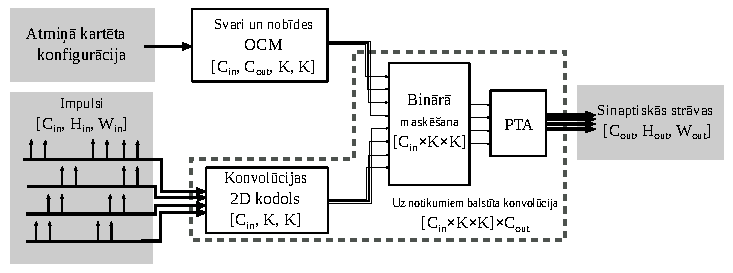
\includegraphics[width=\columnwidth]{fig/lv/conv_layer-v1.pdf}
  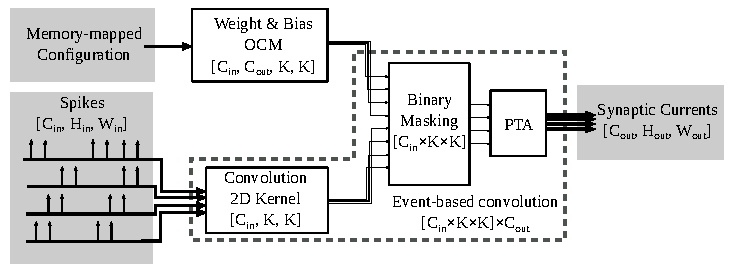
\includegraphics[width=\columnwidth]{fig/conv_layer-v1.pdf}
  \caption{Binārs telpiskais filtrs ar uz notikumiem balstītām konvolūcijām.}
  \label{fig:bsf_arch}
\end{figure}

Konvolūcijas 2D kodols savāc \(K \times K\) telpisko logu no katra ieejas impulsu pazīmju kartes kanāla \(C_{in}\). Impulsi tiek straumēti pa AXI-Stream saskarni uz binārās maskēšanas bloku, savukārt svariem izmanto otru straumēšanas saskarni.

Resursu taupīšanai maskēšanas un \Gls{pta} operācijas tiek veiktas secīgi katram ieejas kanālam \([C_{in}, K, K]\) kodolā un multipleksētas laikā starp \(C_{out}\) izejas kanāliem, kā parādīts \ref{fig:conv_steps}. attēlā. Tas ļauj atkārtoti izmantot to pašu apstrādes loģiku, būtiski samazinot nepieciešamo aparatūras resursu apjomu. Lai samazinātu izpildes laiku, laikā multipleksētā loģika netiek darbināta neaktīvajos laika soļos, izvairoties no nevajadzīgiem aprēķiniem, ja nav ieejas impulsu.

\begin{figure}[htbp]
  % 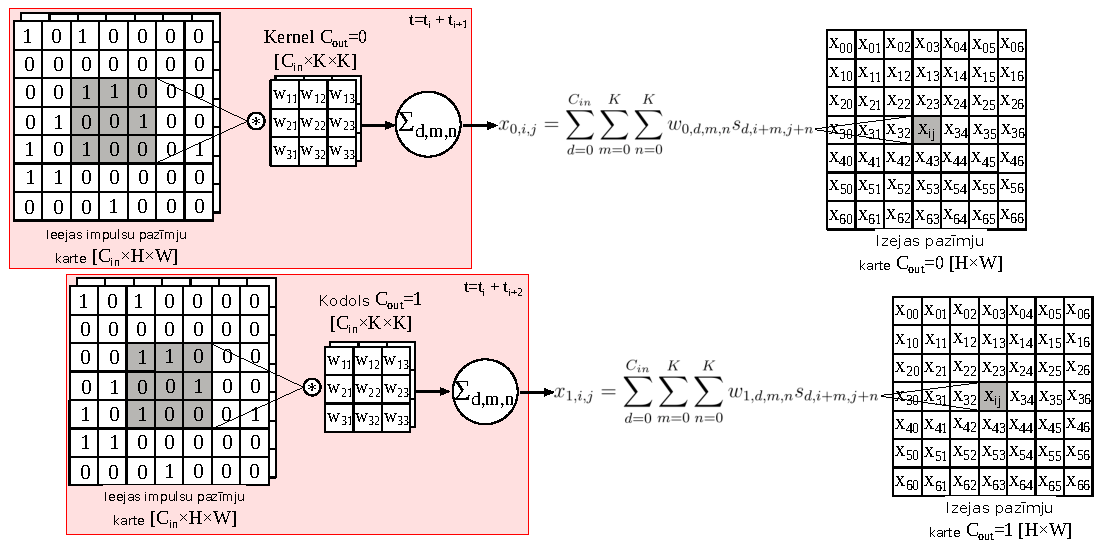
\includegraphics[width=\columnwidth]{fig/lv/conv_time_steps-v2.pdf}
  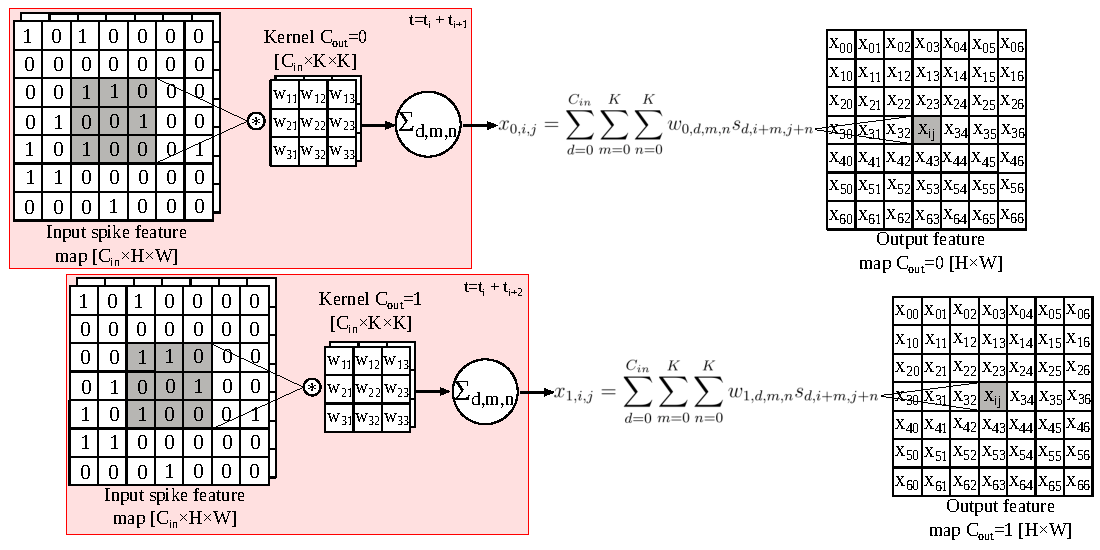
\includegraphics[width=\columnwidth]{fig/conv_time_steps-v2.pdf}
  \caption{Retināta konvolūcija ar līdzsvarotu paralēlismu un resursu atkārtotu izmantošanu: paralēla ieejas kanālu apstrāde un laikā multipleksēta izejas kanālu apstrāde.}
  \label{fig:conv_steps}
\end{figure}

Konvolūcijas soli, kanālu skaitu un ieejas attēla izmērus izpildes laikā var pārkonfigurēt ar īpašiem konfigurācijas reģistriem, novēršot atkārtotas sintēzes nepieciešamību.

Šī moduļa izeja ir sinaptiskās strāvas vektors ar \(C_{out}\) izejas kanāliem, kas pēc tam kalpo par ieeju nākamajiem \Gls{lif} integrēšanas un sliekšņa salīdzināšanas blokiem.



  \subsubsection{Integrējošā neirona ar noplūdi realizācija}
  Šajā darbā LIF neirona digitālās shēmas realizācija ir pielāgota dziļo neironu tīklu realizācijai ar vairākiem 2D telpiskiem
slāņiem. Šādos slāņos glabājamo membrānas potenciālu apjoms pieaug līdz ar kanālu skaitu un pazīmju kartes augstumu un
platumu \(C_{out}, H_{out}, W_{out}\). Tādēļ izmantots \Gls{lif} neirons ar straumējamu membrānas potenciālu, izmantojot ārējo
SDRAM atmiņu.

\Gls{lif} neirona bloka arhitektūra parādīta \ref{fig:lif_arch}. attēlā. Šis integrēšanas un sliekšņa salīdzināšanas bloks
realizē \Gls{lif} neironu uzvedību. Tas integrē ieejas sinaptiskās strāvas, atjaunina membrānas potenciālus un salīdzina tos ar
slieksni, lai noteiktu impulsu ģenerēšanu. \Gls{lif} modelis izvēlēts tā līdzsvara dēļ starp aprēķinu vienkāršību un funkcionālo elastību.

\Gls{lif} aparatūras modulis diskrētā laikā realizē \Gls{lif} neirona modeli, ko nosaka (\ref{eq:lif_v}) un
(\ref{eq:lif_spike}). Modulis integrē sinaptisko ieejas strāvu \(X_o[t]\) laikā \(t\) katram no \(C_{out}\) izejas kanāliem,
iegūstot atjauninātu membrānas potenciālu. Pamatojoties uz membrānas potenciālu un impulsu ģenerēšanas slieksni, katram
izejas kanālam tiek ģenerēta impulsu aktivitāte. Katram slānim kopīgu parametru \(\beta^l\) var konfigurēt pēc sintēzes,
nodrošinot katra slāņa temporālu pielāgošanu. Lai taupītu \Gls{dsp} resursus, \(\beta^l\) tiek ierobežots līdz tuvākajai divnieka pakāpei, kā parādīts (\ref{eq:quant_beta}).

\begin{figure}[ht]
  \centering
  % 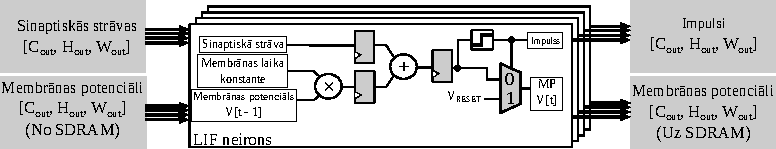
\includegraphics[width=\linewidth]{fig/lv/lif_neuron_core-v4.pdf}
  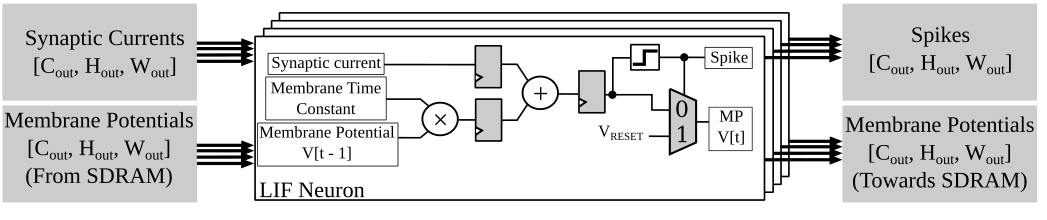
\includegraphics[width=\linewidth]{fig/lif_neuron_core-v4.png}
  \caption{LIF sliekšņa salīdzināšanas bloka aparatūras realizācija, kas atkārtota \(C_{out}\) reizes, ar membrānas potenciālu ārēju straumēšanu temporālai apstrādei ar stāvokļa saglabāšanu.}
  \label{fig:lif_arch}
\end{figure}

Vienu ieejas straumi izmanto sinaptiskajām strāvām \(X_o[t]\) no binārā telpiskā konvolūcijas filtra, savukārt otru straumi ārējai SDRAM atmiņai izmanto iepriekšējā laika soļa membrānas potenciālu \(V[t-1]\) ielādei un pašreizējo membrānas potenciālu \(V[t]\) ierakstīšanai atpakaļ. Abas straumes sinhronizē ar AXI-Stream sinhronizatoru, lai nodrošinātu pareizu laika saskaņojumu. Katrā slānī sliekšņa salīdzināšanas struktūra tiek atkārtota \(C_{out}\) reizes paralēlai apstrādei. Lai gan iepriekšējos darbos \cite{zhang2024, sommer2022} membrānas potenciāli tiek glabāti lokāli mikroshēmas iekšējā atmiņā tuvu apstrādes elementiem, lai samazinātu latentumu, BRAM izmantojums var strauji sasniegt pieejamo robežu, un risinājums slikti mērogojas līdz ar tīkla izmēru. Nepieciešamās atmiņas apjoms pieaug proporcionāli \(C_{out} \times H \times W\) un slāņu skaitam. Tādēļ piedāvātajā risinājumā mikroshēmas iekšējā BRAM glabā tikai konvolūcijas svarus, savukārt membrānas potenciāli tiek straumēti uz ārējo atmiņu un no tās.

Pēc membrānas integrēšanas un salīdzināšanas ar slieksni neirons ģenerē binārus izejas impulsus. Šos impulsus var novirzīt vai nu uz nākamo iekšējo slāni, vai uz AER kodētāja ieejas portu pārraidei kā ārējiem notikumiem.

Pēc izvēles ģenerētajām impulsu pazīmju kartēm var piemērot apvienošanas posmu, lai samazinātu to telpiskos izmērus. Apvienošanas slānis veic maksimuma apvienošanu konfigurējamā kodola logā ar programmējamu soli. Bināru impulsu reprezentācijām maksimuma apvienošana vienkāršojas līdz loģiskajai VAI operācijai pa elementiem apvienošanas logā. Tā kā bināru vērtību kopas maksimums ir viens ikreiz, kad logā ir aktīvs vismaz viens impulss, apvienošanas izeju var pierakstīt šādi:
\begin{equation}
  s_{\text{pool}} = \max(s_1, s_2, \ldots, s_n) = s_0 \vee s_1 \vee \ldots \vee s_n,
\end{equation}
kur \(\vee\) ir loģiskais VAI operators un \(n\) ir neironu skaits apvienošanas logā. Būtiski, ka apvienošanas bloku aparatūrā var realizēt ar vienkāršu kokveida VAI vārtu struktūru, izvairoties no aritmētiskām salīdzināšanas operācijām un saglabājot impulsu aktivitāti uztveres laukā. Šī operācija saglabā impulsu aktivitātes klātbūtni uztveres laukā, vienlaikus samazinot pazīmju karšu telpisko izšķirtspēju.



  % \subsubsection{Ižikeviča impulsu neirona realizācija}
  % Eilera metodi \cite{burden2011} var izmantot neirona modeļa aproksimāciju aprēķināšanai pie jebkuras dotas vērtības. Piemērojot Eilera metodi \eqref{eq:izhi}, iegūst diskrēta laika vienādojumus membrānas potenciāla un atjaunošanās mainīgā vērtībām:
\begin{equation}
  \label{eq:discrete_uv}
  \begin{cases}
  v_{n + 1} = v_{n} + \Delta t(0{,}04v_{n}^{2} + 5v_{n} + 140 - u_{n} + I) \\
  u_{n + 1} = u_{n} + \Delta ta(bv_{n} - u_{n}).
  \end{cases}
\end{equation}

Eilera metode ir pirmās kārtas metode, kas nozīmē, ka lokālā diskretizācijas kļūda \(e(\Delta t)\) ir saistīta ar soļa lielumu kā \(e(\Delta t)=O(\Delta t^2)\), bet globālā diskretizācijas kļūda \(E(\Delta t)\) — kā \(E(\Delta t)=O(\Delta t)\). Jāņem vērā, ka lokālo kļūdu ietekme uzkrājas, jo turpmākajos aprēķinos tiek izmantotas noapaļotas vērtības. Praksē arī fiksētā komata noapaļošanas kļūda ietekmē globālo kļūdu, kura tad vairs nav lineāra attiecībā pret \(\Delta t\). Mazāka soļa izvēle sāks palielināt \(E(\Delta t)\), ja fiksētā komata precizitātes kļūda nebūs pietiekami maza salīdzinājumā ar soli. Šī ietekme jāņem vērā, nosakot atbilstošu fiksētā komata mainīgā un soļa lielumu.

Vienādojumu \eqref{eq:discrete_uv} var pārkārtot, aizstājot parametrus \(b\), \(I\) ar \(b^{*}=\Delta tb\) un \(I^{*}=\Delta tI\). Turklāt reizināšanu ar koeficientu \(0{,}04\Delta t\) var aizstāt ar nobīdes operāciju, izvēloties \(\Delta t\) tā, lai koeficients precīzi atbilstu divnieka pakāpei. Lai gan tas ierobežo laika soļa izšķirtspēju, reizināšanas operācijas ir precīzas un var izvēlēties arvien mazākas \(\Delta t\) vērtības. Abi realizējamie aprēķinu konveijeri kļūst par:
\begin{equation}
\label{eq:discrete_fe_uv}
\begin{cases}
  v_{n + 1} = v_{n} + v_{n}^{2}\gg n + 5\Delta tv_{n} + 140\Delta t - u_{n}^{*} + I^{*} \\
  u_{n + 1} = u_{n}^{*} + a(b^{*}v_{n} - u_{n}^{*}),
\end{cases}
\end{equation}
kur \(n\) ir pozīciju skaits, par kuru nobīdīt \(v^{2}_{n}\), un \(\gg\) ir binārā nobīde pa labi. Pārējās reizināšanas operācijas tiek saglabātas, un tās var realizēt ar aparatūras reizinātājiem vai \Gls{cordic} reizinātājiem, lai saglabātu precizitāti un parametru pielāgošanas elastību.

Vienādojuma (\ref{eq:discrete_fe_uv}) digitālās shēmas realizācija redzama \ref{fig:izhikevich_impl}. attēlā. Tā kā viens tipisks reizinātājs (piemēram, \Gls{dsp} kodols \textit{Xilinx Kintex} \Gls{fpga}) spēj veikt 18 bitu operācijas, katra reizinātāja operanda fiksētā komata vērtība ir ierobežota ar 18 bitu reprezentāciju. Šajā gadījumā viens reizinātājs tiek multipleksēts laikā, lai taupītu DSP bloku resursus. Salīdzinājumā ar citiem darbiem šis risinājums ļauj pielāgot laika soli uz lielāka aprēķinu latentuma rēķina. Var izmantot katru laika soli \(\Delta t = 2^{n}/0{,}04\), ja nobīdes operāciju skaits \(n\) ir vesels skaitlis.

\begin{figure}[htbp]
  \centering
  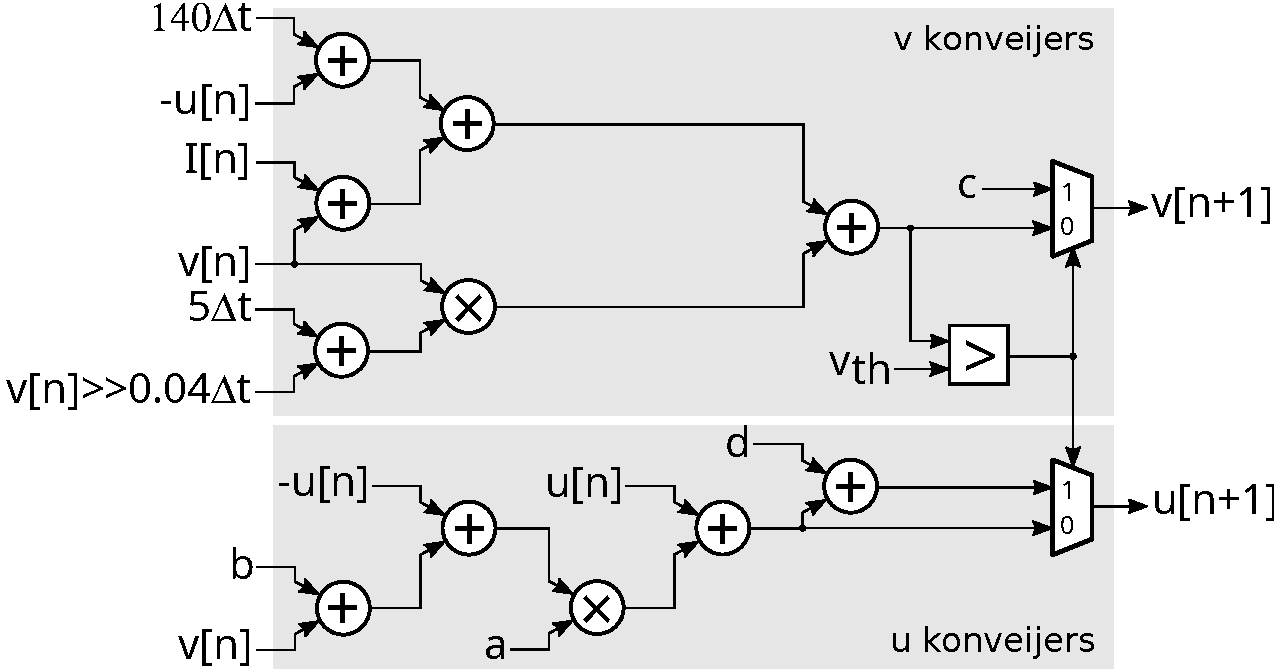
\includegraphics[width=0.7\columnwidth]{fig/lv/izh_impl_v2.pdf}
  \caption{Ižikeviča neirona realizācija, izmantojot tiešo Eilera metodi, kas optimizēta mainīgai precizitātei.}
  \label{fig:izhikevich_impl}

  \vspace{-0.5cm}
\end{figure}



  \subsubsection{SNN kvantēšana realizācijai aparatūrā}
  

Dziļie konvolucionālie \Gls{snn} modeļi bieži satur lielu parametru skaitu, kas ievērojami palielina nepieciešamos skaitļošanas resursus. Izmantojot
kvantēšanas metodes, parametru reprezentāciju parasti var būtiski samazināt no 32 bitu peldošā punkta līdz maza bitu platuma
reprezentācijai (piemēram, 4 vai 8 bitiem), būtiski nesamazinot veiktspēju \cite{wei2024}. Lai taupītu atmiņu un skaitļošanas
resursus, konvolūcijas kodolu svariem un nobīdēm piemēro kvantēšanu, kas samazina bitu platumu tā, lai šis samazinājums
būtiski neietekmētu veiktspēju. Tas ir īpaši svarīgi, realizējot \Gls{snn} \Gls{fpga} paātrinātājos un glabāšanai izmantojot
\Gls{ocm}.

Divas bieži izmantotas metodes ir \Gls{ptq} un \Gls{qat}. Izmantojot \Gls{ptq}, tīklu vispirms apmāca ar tradicionāliem
peldošā punkta parametriem un pēc tam apmācītos svarus pārveido zemākas precizitātes reprezentācijā \cite{zhou2016}. Šī pieeja neprasa izmaiņas apmācības procesā un ļauj novērtēt dažādas kvantēšanas precizitātes uzreiz pēc modeļa apmācības. Tomēr kvantēšana ar mazu bitu skaitu var izraisīt precizitātes samazinājumu, ko pēc apmācības vairs nevar uzlabot. Savukārt \Gls{qat} gadījumā kvantēšanas ietekme tiek iekļauta apmācībā, ļaujot svariem pielāgoties kvantēšanas kļūdai un uzlabot precizitāti pie maza bitu platuma \cite{zhou2016, plagwitz2024}. Tomēr \Gls{qat} lielākā apmācības sarežģītība padara \Gls{ptq} vēlamāku, ja aparatūras realizācijas novērtē vairākos precizitātes līmeņos.

Reāli peldošā punkta skaitļi tiek kvantēti uz $k$ bitu reprezentāciju \cite{zhou2016}:

\begin{equation}
  Q(w) =  \frac{1}{2^{k - 1}} clip(\lfloor w \cdot 2^{k}-1 \rceil, 0, 2^{k}-1)
\end{equation}
kur \(\lfloor \cdot \rceil\) apzīmē noapaļošanas operāciju. Ieeja diapazonā \(w \in [0, 1]\) tiks kvantēta uz tuvāko \(i / (2^{k} - 1)\), kur \(i = 0, 1, ..., (2^{k} - 1)\).



\subsection{Telpiski temporāla objektu detektēšana ar dziļiem impulsu CNN, izmantojot punktu mākoņu datus}
  Šajā sadaļā aplūkota \Gls{snn} izmantošana attēlu atpazīšanas uzdevumos, īpašu uzmanību pievēršot šī promocijas darba ieguldījumam. Aplūkotie darbi ietver uz \Gls{snn} balstītu attēlu atpazīšanu, objektu detektēšanu retinātos punktu mākoņos ar \Gls{snn} \cite{lielamurs2024} un paplašinājumus uz \Gls{snn} balstītai 3D objektu detektēšanai, kā aprakstīts darbā \cite{lielamurs2025}. Turklāt darba \cite{druml2025} sadaļās par asinhronu notikumu kameru ietvaru pētīta hibrīda pieeja, kas apvieno notikumu vadītus \Gls{snn} ar kadru apstrādi, izmantojot \Gls{resnet} arhitektūru.

  \subsubsection{Vokseļu režģa priekšapstrāde}
  Impulsu kodēšana ir būtiska \Gls{snn} sastāvdaļa, kas nosaka informācijas pārraides veidu ar diskrētiem impulsu laikiem. Dati jākodē impulsu virknēs, lai 3D punktu mākonis tiktu pārveidots laika informācijā \cite{safa2021}. Izmantota \Gls{tvc} metode, kas retinātus telpiski temporālus datus pārveido režģveida formātā nelielā laika soļu skaitā. Līdzīga pieeja atrodama darbos \cite{Cordone2022, fan2025}, kur to sauc par vokseļu kuba kodēšanu. Salīdzinājumā ar parasto vokseļu režģa kodēšanu \cite{bardow2016} vokseļu kuba kodēšana ļauj katrā laika solī kanālu dimensijā glabāt vairāk informācijas.

Veicot šo pārveidošanu, iegūst telpiskās informācijas vairāku soļu impulsu reprezentāciju. Šāda kodēšanas metode izmanto \Gls{snn} rekurento dabu.

Pirms pārveidošanas nepārtrauktā ģeometriskā punktu mākoņa reprezentācija vispirms tiek retināta, iegūstot jaunu diskrētu 3D režģa reprezentāciju, lai samazinātu turpmāko operāciju ieejas datu apjomu. Šādi samazinās atmiņas un skaitļošanas prasības bez būtiska informācijas zuduma, ja vokseļa izmērs ir izvēlēts pareizi. Ja dots sākotnējais nepārtrauktais punktu mākonis 3D telpā \(\mathcal{P} = \{(x_i, y_i, z_i) \mid x_i, y_i, z_i \in \mathbb{R}\}\) un vokseļa izmērs \([VS_x, VS_y, VS_z]\), vokseļu režģi var definēt kā šo punktu diskrētu attēlojumu 3D režģī \(\mathcal{V} = \{(x_v, y_v, z_v) \mid x_v, y_v, z_v \in \mathbb{Z}\}\). Pāreju no nepārtrauktās telpas uz vokseļu telpu attiecībā pret sākotnējā punktu mākoņa minimālajām koordinātām nosaka
\begin{equation}
  \begin{split}
    x_v = \floor*{\frac{x - x_{min}}{VS_x}},
    y_v = \floor*{\frac{y - y_{min}}{VS_y}},
    z_v = \floor*{\frac{z - z_{min}}{VS_z}}
  \end{split}
\label{eq:voxels}
\end{equation}
kur minimālās un maksimālās koordinātas ainā ir
$$[(x_{min}, y_{min}, z_{min}), (x_{max}, y_{max}, z_{max})].$$
Šīs ietverošā paralēlskaldņa vērtības nosaka vokseļu režģa telpiskās robežas un ietekmē vokselizētās reprezentācijas izšķirtspēju. Tā kā vokseļa izmērs īpaši būtiski ietekmē XY plaknes izšķirtspēju, ietverošā paralēlskaldņa apjoms pēc iespējas tiek samazināts, lai līdzsvarotu aprēķinu efektivitāti un telpisko precizitāti. Ar šo metodi tīkls var novērtēt nelielu skaitu \(C \times H \times W\) formas \Gls{bev} pseidoattēlu. Iegūto diskrēto laika soļu skaits ir
\begin{equation}
  T = \frac{z_{max} - z_{min}}{VS_z}.
  \label{eq:T}
\end{equation}

Vokselizācijas process tiek paplašināts ar papildu kvantēšanu, sīkāk sadalot \(T\) laika soļus laika intervālos. Tas ietver z dimensijas sadalīšanu \(n\) diskrētos intervālos:
\begin{equation}
    t_{bin} = \floor*{\frac{(z - z_{min})\ \mathrm{mod}\ VS_z}{Q}},
    \label{eq:bins}
\end{equation}
kur \(Q = VS_z/n\) ir intervāla izmērs. Lieki aprēķini tiek papildus novērsti, apvienojot operācijas vienādojumos (\ref{eq:voxels}) un (\ref{eq:bins}). Šī modifikācija ļauj iegūt detalizētāku informāciju z dimensijā, pielāgojot detalizācijas pakāpi. Ar šo reprezentāciju izveido 4D tenzoru ar formu \(T \times C \times H \times W\), kur \(H\) un \(W\) ir datu augstums un platums, \(C\) ir kanālu skaits katrā laika solī un \(T\) ir laika soļu skaits. Sīkāk sadalot vokseļus un glabājot papildu informāciju kanālu dimensijā, vokseļu intervāli ļauj palielināt izšķirtspēju, nepalielinot laika soļu skaitu.

Ja LiDAR vietā izmanto \Gls{tof} datus, kā parādīts \ref{fig:3dscnn_tof_arch}. attēlā, datus iegūst no vairākiem izkliedētiem sensoriem. Pirms temporālās vokselizācijas atsevišķie punktu mākoņi jāpārveido kopīgā koordinātu sistēmā. Katram sensoram stingro transformāciju aprēķina no blakus esošo sensoru pārklāšanās apgabala. Reģistrācijas procedūrā punktu mākoņu transformāciju pārus novērtē, identificējot atbilstošas ģeometriskās pazīmes. Šajā darbā tam izmanto \Gls{dgr}, ievērojot uz pazīmēm balstītu punktu mākoņu reģistrācijas pieeju, kas aprakstīta darbos \cite{choy2020, choy2019a, choy2019b, li2021}. Transformācijas piemēro atsevišķajiem punktu mākoņiem, iegūstot vides reprezentāciju kopīgā koordinātu sistēmā.

\begin{figure}[ht]
    \centering
    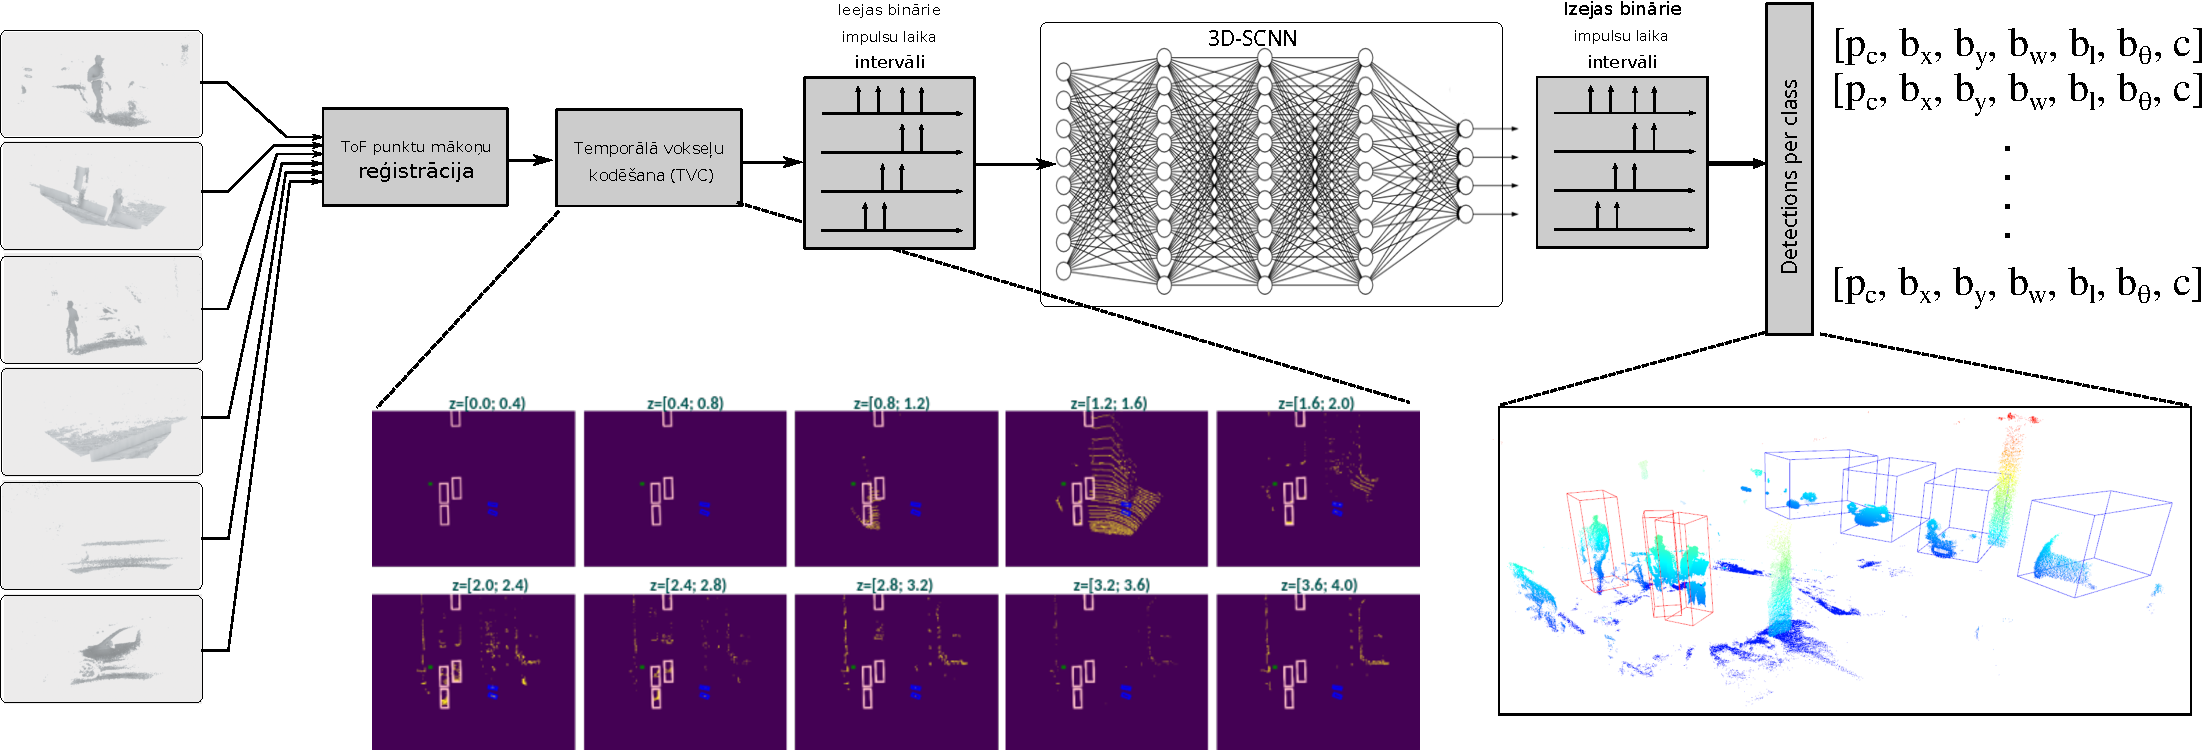
\includegraphics[width=\textwidth]{fig/lv/3dscnn_architecture-v3.pdf}
    \caption{3D-CSNN arhitektūra. Vairāku ToF sensoru nepārtrauktā punktu mākoņu telpa tiek reģistrēta un retināta, izveidojot diskrētus režģus vairākos laika soļos objektu detektēšanai ar 3D konvolucionālu \Gls{snn}.}
    \label{fig:3dscnn_tof_arch}
\end{figure}



  \subsubsection{Impulsu konvolūcijas slāņi}
  Konvolūcijas slāņus plaši izmanto \Gls{snn} arhitektūrās, parasti aizstājot \Gls{relu} aktivācijas ar integrējošiem impulsu
neironiem ar noplūdi \cite{cao2015}. Šādi tīkli objektu detektēšanā notikumu attēlu datu kopās pārspēj tradicionālos
\Gls{ann} \cite{zhang2023}. Turklāt dziļi tīkli, kas papildināti ar pakešu normalizāciju, ir būtiski detektēšanas
precizitātes uzlabošanai ainās ar daudzām detaļām \cite{kim2021}. Iepriekšējos pētījumos \cite{sengupta2019, kim2021,
Cordone2022} demonstrēts, ka attīstītas \Gls{ann} topoloģijas, piemēram, \textit{VGG}, var izmantot pazīmju iegūšanai un
apvienot ar \Gls{ssd} objektu detektēšanai no iegūtajām pazīmēm. Tradicionālo aktivācijas funkciju, piemēram, \Gls{relu},
vietā šie modeļi izmanto temporālus vairāku soļu \Gls{lif} neironus. Jāatzīmē, ka \Gls{ssd} objektu detektēšanas galva
izmantota ar impulsu \textit{DenseNet} un \textit{ResNet} arhitektūru variantiem. Šajā darbā impulsu \textit{VGG} veiktspēja
novērtēta 3D informācijas uztverē, aktivācijas funkcijas aizstājot ar \Gls{lif} neironiem ar apmācāmu membrānas laika
konstanti.

Impulsu \Gls{cnn} sastāv no konvolūcijām, maksimuma apvienošanas, pakešu normalizācijas un impulsu neironiem. Pamattīklā izmantotais apstrādes pamatbloks ilustrēts \ref{fig:spiking_conv_block}. attēlā. Impulsu konvolucionālā tīkla ieeja ir temporāls binārs tenzors \(\mathbf{X}\in\{0,1\}^{T\times C\times H\times W}\). Impulsu neirons saglabā stāvokli, un tā membrānas potenciāls mainās laikā, tādēļ \Gls{snn} līdzinās bināriem \Gls{rnn} \cite{neftci2019}. Izmantojot impulsu neironu rekurento dabu, 2D konvolūcijas atkārto vairākos \Gls{bev} šķēlumos, kas reprezentē \(T\) laika soļus ar \(C\) kanāliem katrā, kā iegūts ar diskrēto reprezentāciju vienādojumos (\ref{eq:T}) un (\ref{eq:bins}). Tā kā konvolūcijas svari ir kopīgi visiem laika soļiem, pati konvolūcija neatkarīgi iegūst telpiskās pazīmes katrā laika solī \(T\), savukārt \Gls{lif} neironu membrānas stāvoklis nodrošina temporālo integrāciju starp soļiem. Tādējādi punktu mākoņu apstrādei tīkls izmanto 2D konvolūcijas skaitļošanas ziņā dārgu 3D konvolūciju vietā. Telpiskās \(X\) un \(Y\) dimensijas reprezentē \Gls{bev} pazīmju karte, savukārt trešā telpiskā dimensija \(Z\) tiek kodēta laikā \(T\) kadru virknē.

\begin{figure}[t]
    \centering
    % 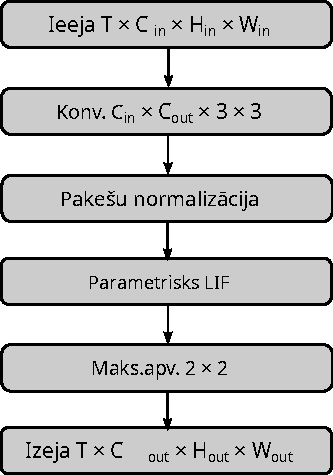
\includegraphics[width=0.25\linewidth]{fig/lv/layer_slice.pdf}
    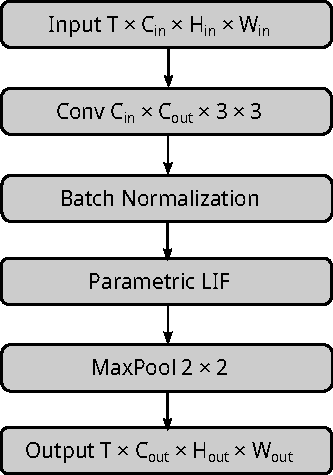
\includegraphics[width=0.25\linewidth]{fig/layer_slice.pdf}
    \caption{Impulsu konvolūcijas pamatbloks, kas sastāv no konvolūcijas, pakešu normalizācijas, LIF neirona un maksimuma apvienošanas operācijas.}
    \label{fig:spiking_conv_block}
\end{figure}

Apmācības laikā pēc konvolūcijām piemēro pakešu normalizāciju, lai uzlabotu zuduma funkcijas optimizāciju un stabilizētu aktivāciju sadalījumu tīklā \cite{ioffe2015}. Inferences laikā pakešu normalizācijas parametri tiek apvienoti ar konvolūcijas slāni, tādēļ aparatūras realizācijai nav nepieciešams atsevišķs normalizācijas slānis.

Pēc pakešu normalizācijas slāņiem seko \Gls{lif} impulsu neironu slāņi \cite{Fang2021}. Šajā darbā izmantoti adaptīvi \Gls{lif} neironi. Uzlabojot tradicionālos \Gls{lif} neironus ar fiksētiem parametriem, membrānas laika konstante tiek apgūta apmācības laikā. Membrānas stāvokli var izteikt šādi \cite{Fang2021}:
\begin{equation}
    U[t] = \beta U[t-1](1-S[t-1]) + I[t],
\end{equation}
kur \(\beta\) ir apmācāms membrānas dilšanas parametrs, \(I[t]\) ir sinaptiskā ieeja un \(S[t]\) ir izejas impulss. Parametra \(\beta\) apmācība ļauj atsevišķiem neironiem pielāgot temporālās integrēšanas īpašības ieejas datu telpiski temporālajām īpašībām.

Līdzīgi kā tradicionālajos \Gls{cnn}, pēc impulsu neironu slāņiem seko maksimuma apvienošanas operācijas \cite{Fang2021}, lai samazinātu dimensijas un iegūtu galvenās pazīmes no impulsu virknēm.

Pamattīklam tiek pievienoti papildus konvolūcijas slāņi, kas pakāpeniski samazina telpisko izšķirtspēju un ģenerē vairāku
mērogu pazīmju kartes, līdzīgi kā \Gls{ssd} arhitektūrās \cite{liu2016}. Šos papildu slāņus izmanto objektu detektēšanai
dažādos mērogos, nodrošinot pazīmju reprezentācijas ar dažādiem uztveres laukiem.



  \subsubsection{Detektēšana un klasifikācija}
  Vairumā temporālās kodēšanas gadījumu pēdējā slānī izmanto impulsu akumulatoru \cite{Fang2021, kim2021, rathi2020}. Galīgo izeju aprēķina kā vairāku impulsu summu visos \(T\) laika soļos, lai veicinātu visaugstāko impulsu ģenerēšanas biežumu neironam, kas saistīts ar sagaidāmo izeju.

Impulsu pamattīkla izejas impulsi tiek pārveidoti uzkrātā pazīmju reprezentācijā, pirms tos nodod \Gls{ssd} detektēšanas galvai. Izeja tiek vidējota visos \(T\) laika soļos. Izejas pazīmju kartei ar kanālu \(c\) un telpiskajām koordinātām \(h, w\) laikā vidējoto pazīmju reprezentāciju nosaka
\begin{equation}
    F_{c,h,w} =
    \frac{1}{T}\sum_{t=0}^{T-1} S_{t,c,h,w},
\end{equation}
kur \(S_{t,c,h,w}\in\{0,1\}\) ir neirona izejas impulss laika solī \(t\). Iegūtā \(F\) reprezentē impulsu pazīmju kartes vidējo impulsu aktivitāti. Pēc tam detektēšanas galva veic objektu klasifikāciju, ietverošo taisnstūru regresiju un orientācijas novērtēšanu.

Ietverošo taisnstūru detektēšanai un klasifikācijai izmanto \Gls{ssd} \cite{liu2016} prognozēšanas galvas. Tās saņem \Gls{snn} pamattīkla ģenerētās pazīmju kartes, nodrošinot vienlaicīgu objektu detektēšanu un to ietverošo taisnstūru regresiju. Paplašinot iepriekšējos darbus \cite{Cordone2022, fan2025}, arhitektūra papildināta ar orientācijas regresiju, kas piedāvāta darbā \cite{simony2018}, lai detektētu vairāku klašu orientētus ietverošos taisnstūrus. Katram detektētajam objektam detektēšanas galva ģenerē izejas vektoru
\begin{equation}
    d = [p_c, b_x, b_y, b_w, b_l, b_\theta, c],
\end{equation}
kur \(p_c\) ir prognozētā ticamības vērtība, \(b_x\) un \(b_y\) ir ietverošā taisnstūra centra koordinātas \Gls{bev} plaknē, \(b_w\) un \(b_l\) ir tā platums un garums, \(b_\theta\) ir tā orientācijas leņķis attiecībā pret \Gls{bev} koordinātām un \(c\) ir prognozētā objekta klase.

Tīkls tiek apmācīts ar daudzuzdevumu mērķfunkciju, kas apvieno klasifikācijas, ietverošā taisnstūra regresijas un orientācijas regresijas zudumus:
\begin{equation}
  \mathcal{L} =
  \mathcal{L}_{cls}
  + \lambda_{box}\mathcal{L}_{box}
  + \lambda_{ang}\mathcal{L}_{ang},
\end{equation}
kur \(\mathcal{L}_{cls}\) ir objektu klasifikācijas zudums, \(\mathcal{L}_{box}\) ir ietverošā taisnstūra regresijas zudums un \(\mathcal{L}_{ang}\) ir orientācijas regresijas zudums. Koeficienti \(\lambda_{box}\) un \(\lambda_{ang}\) nosaka regresijas locekļu ieguldījumu kopējā apmācības mērķfunkcijā.

Klasifikācijas zudumam \(\mathcal{L}_{cls}\) izmanto fokālo zuduma funkciju \cite{lin2017}, lai samazinātu vieglāk klasificējamu negatīvo piemēru ieguldījumu un risinātu klašu nelīdzsvarotību. Ietverošā taisnstūra un orientācijas regresijai izmanto \textit{Smooth L1} zuduma funkciju tās noturības pret izlecošām vērtībām un stabilās optimizācijas uzvedības dēļ. Tādējādi apvienotā mērķfunkcija apmāca impulsu pamattīklu un detektēšanas galvas iegūt pazīmes un vienlaikus optimizēt objektu lokalizāciju un orientāciju.

\Gls{ssd} klasifikācijas un regresijas galvas veido viens konvolūcijas slāņu posms bez papildu aktivācijas funkcijām starp
tiem. Tas ir īpaši piemēroti ar aparatūru paātrinātiem \Gls{snn}, jo netiek pievienoti aktivācijas posmi, kuriem būtu
nepieciešama papildu stāvokļu glabāšana un aprēķini, tādējādi nodrošinot saderību ar uz notikumiem balstītu apstrādi \Gls{fpga}
realizācijās. Šādās realizācijās svarīgi, lai aparatūras paātrinātājs atbalstītu papildu savienojumus, kas nodrošina piekļuvi
dažādos pamattīkla līmeņos iegūtām daudzlīmeņu pazīmju kartēm.

Lai saglabātu objektu identitāti starp kadriem, detektors apvienots ar vairāku objektu izsekošanas algoritmu
\textit{AB3DMOT} \cite{weng2020}. Izsekotājs no detektēšanas galvas saņem prognozētos orientētos ietverošos taisnstūrus,
klašu marķējumus un ticamības vērtības un sasaista detektējumus starp kadriem, izmantojot konfigurējamu telpiskās līdzības
metriku. Trajektorija tiek apstiprināta pēc noteikta veiksmīgu sasaistījumu skaita un saglabāta ierobežotu kadru skaitu bez
atbilstoša detektējuma.




\section{Eksperimentālie rezultāti}
Šīs nodaļas eksperimentālais novērtējums pārbauda promocijas darba realizācijas, izmantojot \ref{sec:impl}. nodaļā aplūkoto
realizāciju rezultātus. Tā kā piedāvātās realizācijas pievēršas dažādiem neiromorfās skaitļošanas aspektiem, pārbaude
sadalīta trijās saistītās daļās.

Pirmajā daļā pārbaudīts darbā \cite{lielamurs2026} piedāvātais \Gls{fpga} paātrinātājs. Tā realizācijas veiktspēja mērīta ar
attēlu klasifikācijas veiktspējas testiem, analizējot inferences latentumu, caurlaidību, resursu izmantojumu, kvantēšanas ietekmi
un novērtēto enerģijas patēriņu.

Otrajā daļā pārbaudīta piedāvātā telpiski temporālā objektu detektēšanas metode LiDAR punktu mākoņiem \cite{lielamurs2024}. Tajā uzmanība pievērsta detektēšanas precizitātei un salīdzināta dziļo konvolucionālo impulsu neironu tīklu un tradicionālo mākslīgo neironu tīklu veiktspēja \textit{KITTI} datu kopā.

Trešajā daļā pārbaudīta piedāvātā detektēšanas ietvara piemērotība lidojuma laika sensoru datiem \cite{lielamurs2025}. Eksperimentālie rezultāti ar automobiļu \Gls{tof} kameru parāda laikā kodētu \Gls{snn} piemērotību praktiskiem 3D uztveres uzdevumiem.

\subsection{Veiktspējas novērtēšanas metrikas}
\Gls{snn} paātrinātāja, kas ietver gan programmatūras, gen aparatūras koponentes, jānovērtē gan algoritmiskā, gan aparatūras
līmenī. Algoritmiskais novērtējums aplūko tīkla precizitāti un kvantēšanas ietekmi uz to, savukārt aparatūras novērtējums
koncentrējas uz latentumu, caurlaidību, energoefektivitāti un \Gls{fpga} resursu izmantojumu. Šīs metrikas raksturo
kompromisu starp atpazīšanas veiktspēju un aparatūras realizācijas efektivitāti.

% Klasifikācijas veiktspēju novērtē ar F1 rādītāju, kas vienā metrikā apvieno precizitāti un pilnīgumu un ir piemērots datu kopām ar klašu nelīdzsvarotību. Precizitāte raksturo pareizi klasificēto paraugu īpatsvaru starp paraugiem, kas prognozēti kā pozitīvi, savukārt pilnīgums raksturo pareizi identificēto paraugu īpatsvaru starp faktiski pozitīvajiem paraugiem. Dotai klasei precizitāti \(P\) un pilnīgumu \(R\) definē šādi \cite{goodfellow-2016}:
% \begin{equation}
%     P = \frac{TP}{TP + FP}, R = \frac{TP}{TP + FN},
% \end{equation}
% kur \(TP\), \(FP\) un \(FN\) ir attiecīgi patiesi pozitīvo, aplami pozitīvo un aplami negatīvo prognožu skaits. F1 rādītāju aprēķina šādi \cite{goodfellow-2016}:
% \begin{equation}
%     F_1 = \frac{2PR}{P+R}.
% \end{equation}
% Vairāku klašu klasifikācijas uzdevumos metrikas var aprēķināt katrai klasei atsevišķi un vidējot.

Objektu detektēšanas uzdevumos veiktspēju novērtē ar \Gls{ap}, kas raksturo precizitātes un pilnīguma sakarību pie dažādiem
detektēšanas sliekšņiem. Prognozētu ietverošo taisnstūri uzskata par patiesi pozitīvu, ja tas atbilst marķējuma
objektam, pamatojoties uz \Gls{iou}. Tad vidējo precizitāti var izteikt kā laukumu zem precizitātes un pilnīguma līknes
\cite{goodfellow-2016}:
\begin{equation}
    AP = \int_0^1 P_{\mathrm{interp}}(r)\,dr,
\end{equation}
kur \(P_{\mathrm{interp}}(r)\) ir interpolētā precizitāte pie pilnīguma līmeņa \(r\). Novērtējot vairākas objektu klases, klašu vidējo precizitāti aprēķina kā klašu \Gls{ap} vidējo vērtību.

Inferences latentums definēts kā laiks no ieejas parauga nodošanas paātrinātājam līdz izejas saņemšanai:
\begin{equation}
    t_{\mathrm{lat}} = t_{\mathrm{out}} - t_{\mathrm{in}},
\end{equation}
kur \(t_{\mathrm{in}}\) un \(t_{\mathrm{out}}\) ir attiecīgi ieejas un izejas laika zīmogi. Norādītais latentums ietver
kopējo aparatūras izpildes laiku un visas resursdatora un ierīces saziņas aiztures.
% Apstrādes caurlaidība ir sekundē
% apstrādāto paraugu skaits, ko pietiekami lielam iterāciju skaitam var aproksimēt ar \(FPS \approx 1 / t_{\mathrm{lat}}\).

Piedāvāto arhitektūru energoefektivitāti novērtē, izmantojot gan izmērīto \Gls{fpga} jaudas patēriņu, gan vienas inferences
enerģijas analītiskus novērtējumus. Tie sniedz savstarpēji papildinošu informāciju. Jaudas mērījumi raksturo realizēto
aparatūru, bet analītiskie modeļi novērtē aritmētisko operāciju un atmiņas piekļuves enerģiju. Vienai inferencei nepieciešamo
enerģiju iegūst kā
\begin{equation}
    E_{\mathrm{inf}} = P_{\mathrm{avg}}\, t_{\mathrm{lat}},
\end{equation}
kur \(P_{\mathrm{avg}}\) ir vidējais jaudas patēriņš inferences laikā. Analītiskajos novērtējumos atsevišķi nodala sinaptisko
operāciju, neironu stāvokļu atjaunināšanas un atmiņas piekļuves ieguldījumu, savukārt izmērītās vērtības ietver \Gls{fpga}
statisko jaudu un saziņas papildu patēriņu.

Ekvivalentu tradicionālo \Gls{cnn} ar \(N_{FOp}\) peldošā punkta operācijām patērēto enerģiju var novērtēt šādi \cite{dampfhoffer2022}:
\begin{equation}
\begin{split}
  E_{ANN} = & N_{FPOp} \times E_{MAC} \\
            & + N_{MemOp} \times (E_{rdWeights} + E_{rdAct} + E_{wrAct}),
\end{split}
\label{eq:eann}
\end{equation}
kur \(E_{rdWeights}\), \(E_{rdAct}\), \(E_{wrAct}\) un \(E_{MAC}\) apzīmē attiecīgi svaru lasīšanas, aktivāciju lasīšanas, aktivāciju rakstīšanas un \Gls{mac} operācijās patērēto enerģiju. \(N_{FPOp}\) ir sinaptisko operāciju skaits, un \(N_{MemOp}\) ir atmiņas piekļuves operāciju skaits.

Var aplūkot vienas inferences laikā veikto aritmētisko operāciju skaitu. Konvolūcijas slāņiem \(f_{\mathrm{in}}\) apzīmē neirona ieeju skaitu, kas vienāds ar kodola izmēra un ieejas kanālu skaita reizinājumu:
\begin{equation}
  f_{\mathrm{in}} = K^2 C_{\mathrm{in}}.
\end{equation}
Tradicionālajos \Gls{ann} katram sinaptiskajam savienojumam nepieciešama viena reizināšana un viena saskaitīšana. Kopējais
peldošā punkta operāciju skaits vienā inferencē ir \cite{rueckauer2017}
\begin{equation}
  N_{\mathrm{FPOp}} =
  \sum_{l=1}^{L}
  (2f_{\mathrm{in},l}+1)N_l,
\end{equation}
kur \(N_l\) ir neironu skaits slānī \(l\), un papildu loceklis ņem vērā nobīdes pieskaitīšanu. Pilnībā savienotam slānim \(f_{\mathrm{in}}\) ir iepriekšējā slāņa neironu skaits. Kopējais izejas neironu skaits slānī \(l\) ir
\begin{equation}
    N_l = H_l \times W_l \times C_{\mathrm{out},l},
\end{equation}
kur \(H_l\), \(W_l\) un \(C_{\mathrm{out},l}\) ir attiecīgi izejas pazīmju kartes augstums, platums un kanālu skaits.

Atbilstoši darba \cite{horowitz2014} metodoloģijai atmiņas piekļuves un aritmētisko operāciju enerģijas tiek aproksimētas ar
mūsdienu \Gls{cmos} tehnoloģijām raksturīgām vērtībām. Tā kā pieņemts, ka svari un aktivācijas tiek glabāti ārējā SDRAM,
vienas atmiņas piekļuves enerģija pieņemta kā \(E_{rdWeight}=E_{rdAct}=E_{wrAct}=1300\,\mathrm{pJ}\). Tāpat pieņemts, ka 32
bitu peldošā punkta reizināšanas un uzkrāšanas operācijas enerģija ir \(E_{MAC}=4{,}6\,\mathrm{pJ}\). Šīs vērtības nodrošina no tehnoloģijas neatkarīgu analītisku enerģijas novērtējumu un tiek izmantotas līdzvērtīgai \Gls{ann} un \Gls{snn} inferences algoritmisko enerģijas prasību salīdzināšanai.

\Gls{lif} neironu konvolūcijas slānim, kas aprakstīts vienādojumos (\ref{eq:lif_conv}) un (\ref{eq:lif_v}), enerģiju novērtē šādi \cite{dampfhoffer2022}:
\begin{equation}
\begin{split}
  E_{SNN} = & N_{SynOp} \times (E_{rdWeights} + E_{ACC}) \\
            & + N_{Neurons} \times T \times (E_{rdState} + E_{wrState} + E_{ACC}),
\end{split}
\label{eq:esnn}
\end{equation}
kur \(N_{SynOp}\) apzīmē sinaptisko operāciju skaitu, bet locekļi \(E_{rdState}\), \(E_{wrState}\) atbilst enerģijai, kas patērēta attiecīgi sinaptisko svaru lasīšanai, neironu stāvokļu lasīšanai un atjaunināto neironu stāvokļu rakstīšanai. \(E_{ACC}\) apzīmē \Gls{acc} operāciju enerģiju, summējot ieejas bez reizināšanas. \(N_{Neurons}\) ir kopējais neironu skaits tīklā, un \(T\) ir laika soļu skaits.

\Gls{snn} sinaptiskie aprēķini tiek veikti tikai tad, kad rodas impulsi. Kopējais sinaptiskās uzkrāšanas operāciju skaits
inferencē ar \(T\) laika soļiem ir \cite{rueckauer2017}
% \begin{equation}
%   N_{\mathrm{SynOp}} =
%   \sum_{t=1}^{T}
%   \sum_{l=1}^{L}
%   f_{\mathrm{in},l}\,
%   N_{active,l}[t],
% \end{equation}
% kur \(N_{active,l}[t]\) ir neironu skaits, kuru membrānas stāvoklis tiek atjaunināts slānī \(l\) laika solī \(t\), un
% \(f_{\mathrm{in},l}\) ir katra neirona ieeju skaits.
\begin{equation}
    N_{\mathrm{SynOp}} =
    \sum_{l=1}^{L}
    N_{\mathrm{neurons},l} \times
    f_{\mathrm{in},l} \times
    N_{\mathrm{spikes/syn},l},
    \label{eq:snn_synops}
\end{equation}
kur \(N_l\) ir neironu skaits slānī \(l\) un \(N_{\mathrm{spikes/syn},l}\) ir vidējais pulsu skaits uz katru sinapsi
inference laika loga \(T\) laikā.

\Gls{fpga} arhitektūrā konvolūcijas svari tiek glabāti mikroshēmas iekšējā \Gls{bram}, kas modelēta ar SRAM piekļuves
enerģiju \(E_{rdWeight}=10\,\mathrm{pJ}\), savukārt neironu membrānas stāvokļi tiek glabāti ārējā SDRAM, iegūstot
\(E_{rdState}=E_{wrState}=1300\,\mathrm{pJ}\). Impulsu notikumu uzkrāšana aizstāj peldošā punkta \Gls{mac} operācijas, tādēļ atbilstoši darbam \cite{horowitz2014} pieņemta akumulatora enerģija \(E_{ACC}=0{,}9\,\mathrm{pJ}\).

Lai salīdzinātu \Gls{snn} enerģijas patēriņu ar ekvivalentu \Gls{ann} realizāciju, relatīvo inferences enerģijas samazinājumu aprēķina šādi:
\begin{equation}
    R = 1-\frac{E_{\mathrm{SNN}}}{E_{\mathrm{ANN}}}.
    \label{eq:delta_e}
\end{equation}

\Gls{snn} aktivāciju retinājumu novērtē, lai raksturotu aktīvo neironu izeju īpatsvaru. Impulsu slānim \(l\) retinājumu definē šādi \cite{Zhou2020}:
\begin{equation}
  S_l = \frac{1}{T N_l}
    \sum_{t=0}^{T-1}
    \sum_{i=1}^{N_l}
    S_{l,i}[t]
    \label{eq:layer_sparsity}
\end{equation}
kur \(T\) ir simulācijas laika soļu skaits, \(N_l\) ir neironu skaits slānī \(l\) un \(S_{l,i}[t] \in \{0,1\}\) ir slāņa \(l\) neirona \(i\) izejas impulss laika solī \(t\).

Kopējo tīkla retinājumu aprēķina, summējot aktīvos impulsu notikumus visos \(L\) impulsu slāņos:
\begin{equation}
    S_{\mathrm{net}} =
    \frac{
    \displaystyle
    \sum_{l=1}^{L}
    \sum_{t=0}^{T-1}
    \sum_{i=1}^{N_l}
    S_{l,i}[t]
    }{
    \displaystyle T \sum_{l=1}^{L} N_l
    }.
    \label{eq:network_sparsity}
\end{equation}

Visbeidzot realizācijas efektivitāti raksturo \Gls{fpga} resursu izmantojums, tostarp \Gls{lut}, \Gls{ff}, \Gls{bram} un
\Gls{dsp} bloki, kā arī maksimālā sasniedzamā takts frekvence \(f_{\max}\). Šīs metrikas norāda uz piedāvātās arhitektūras
mērogojamību un nosaka lielāku impulsu neironu tīklu realizācijai pieejamos resursus.
% Maksimālo darbības frekvenci nosaka pēc
% izvietošanas un trasēšanas laika parametru analīzes. \(T_{\mathrm{target}}\) apzīmē mērķa takts periodu un \(\mathrm{WNS}\)
% — sliktāko negatīvo laika rezervi, kas noteikta pēc realizācijas. Minimālais iespējamais takts periods ir
% \begin{equation}
%   T_{\min} = T_{\mathrm{target}}-\mathrm{WNS},
% \end{equation}
% kur negatīvs \(\mathrm{WNS}\) norāda uz laika ierobežojumu pārkāpumu. Tātad maksimālā darbības frekvence ir
% \begin{equation}
%   f_{\max} = \frac{1}{T_{\min}}
%   =\frac{1}{T_{\mathrm{target}}-\mathrm{WNS}}.
% \end{equation}



\subsection{Salīdzinoša veiktspējas analīze}
  \subsubsection{Uz PCIe balstīts FPGA paātrinātājs pārkonfigurējamiem konvolucionāliem impulsu neironu tīkliem}
    \paragraph{Eksperimentu konfigurācija}\mbox{} \\
    Paātrinātāja sistēma realizēta VHDL un novērtēta ar reprezentatīviem dziļajiem konvolucionālajiem impulsu neironu tīkliem.
Realizācija sintezēta, izvietota un trasēta ar \textit{AMD Vivado} rīku \textit{Xilinx Kintex UltraScale KU115-2}
\Gls{fpga} iekārtai. Turpmākajās sadaļās norādītais resursu izmantojums, maksimālā darbības frekvence, latentums un jaudas patēriņš
iegūti realizētajam projektam.

Eksperimentālā pārbaude veikta ar \textit{Alpha Data ADM-PCIE-8K5}\footnote{https://alpha-data.com/product/adm-pcie-8k5/}
PCIe paātrinātāja karti, kurā izmantots \textit{Kintex UltraScale KU115-2} \Gls{fpga}. \Gls{fpga} karte uzstādīta
\textit{NVIDIA Jetson AGX Orin}\footnote{https://www.nvidia.com/en-us/autonomous-machines/embedded-systems/jetson-orin/}
iegultajā skaitļošanas platformā, kas kalpo par procesoru un atbild par tīkla konfigurāciju, datu
pārsūtīšanu un rezultātu savākšanu. Saziņa starp to un paātrinātāju notiek pa PCI Express saskarni, savukārt
\Gls{fpga} pēc nepieciešamo konfigurācijas parametru un ieejas impulsu straumju saņemšanas izpilda uz notikumiem balstīto
apstrādi. Eksperimentālā platforma parādīta \ref{fig:fpga_jetson}. attēlā.
\begin{figure}[!t]
\centering
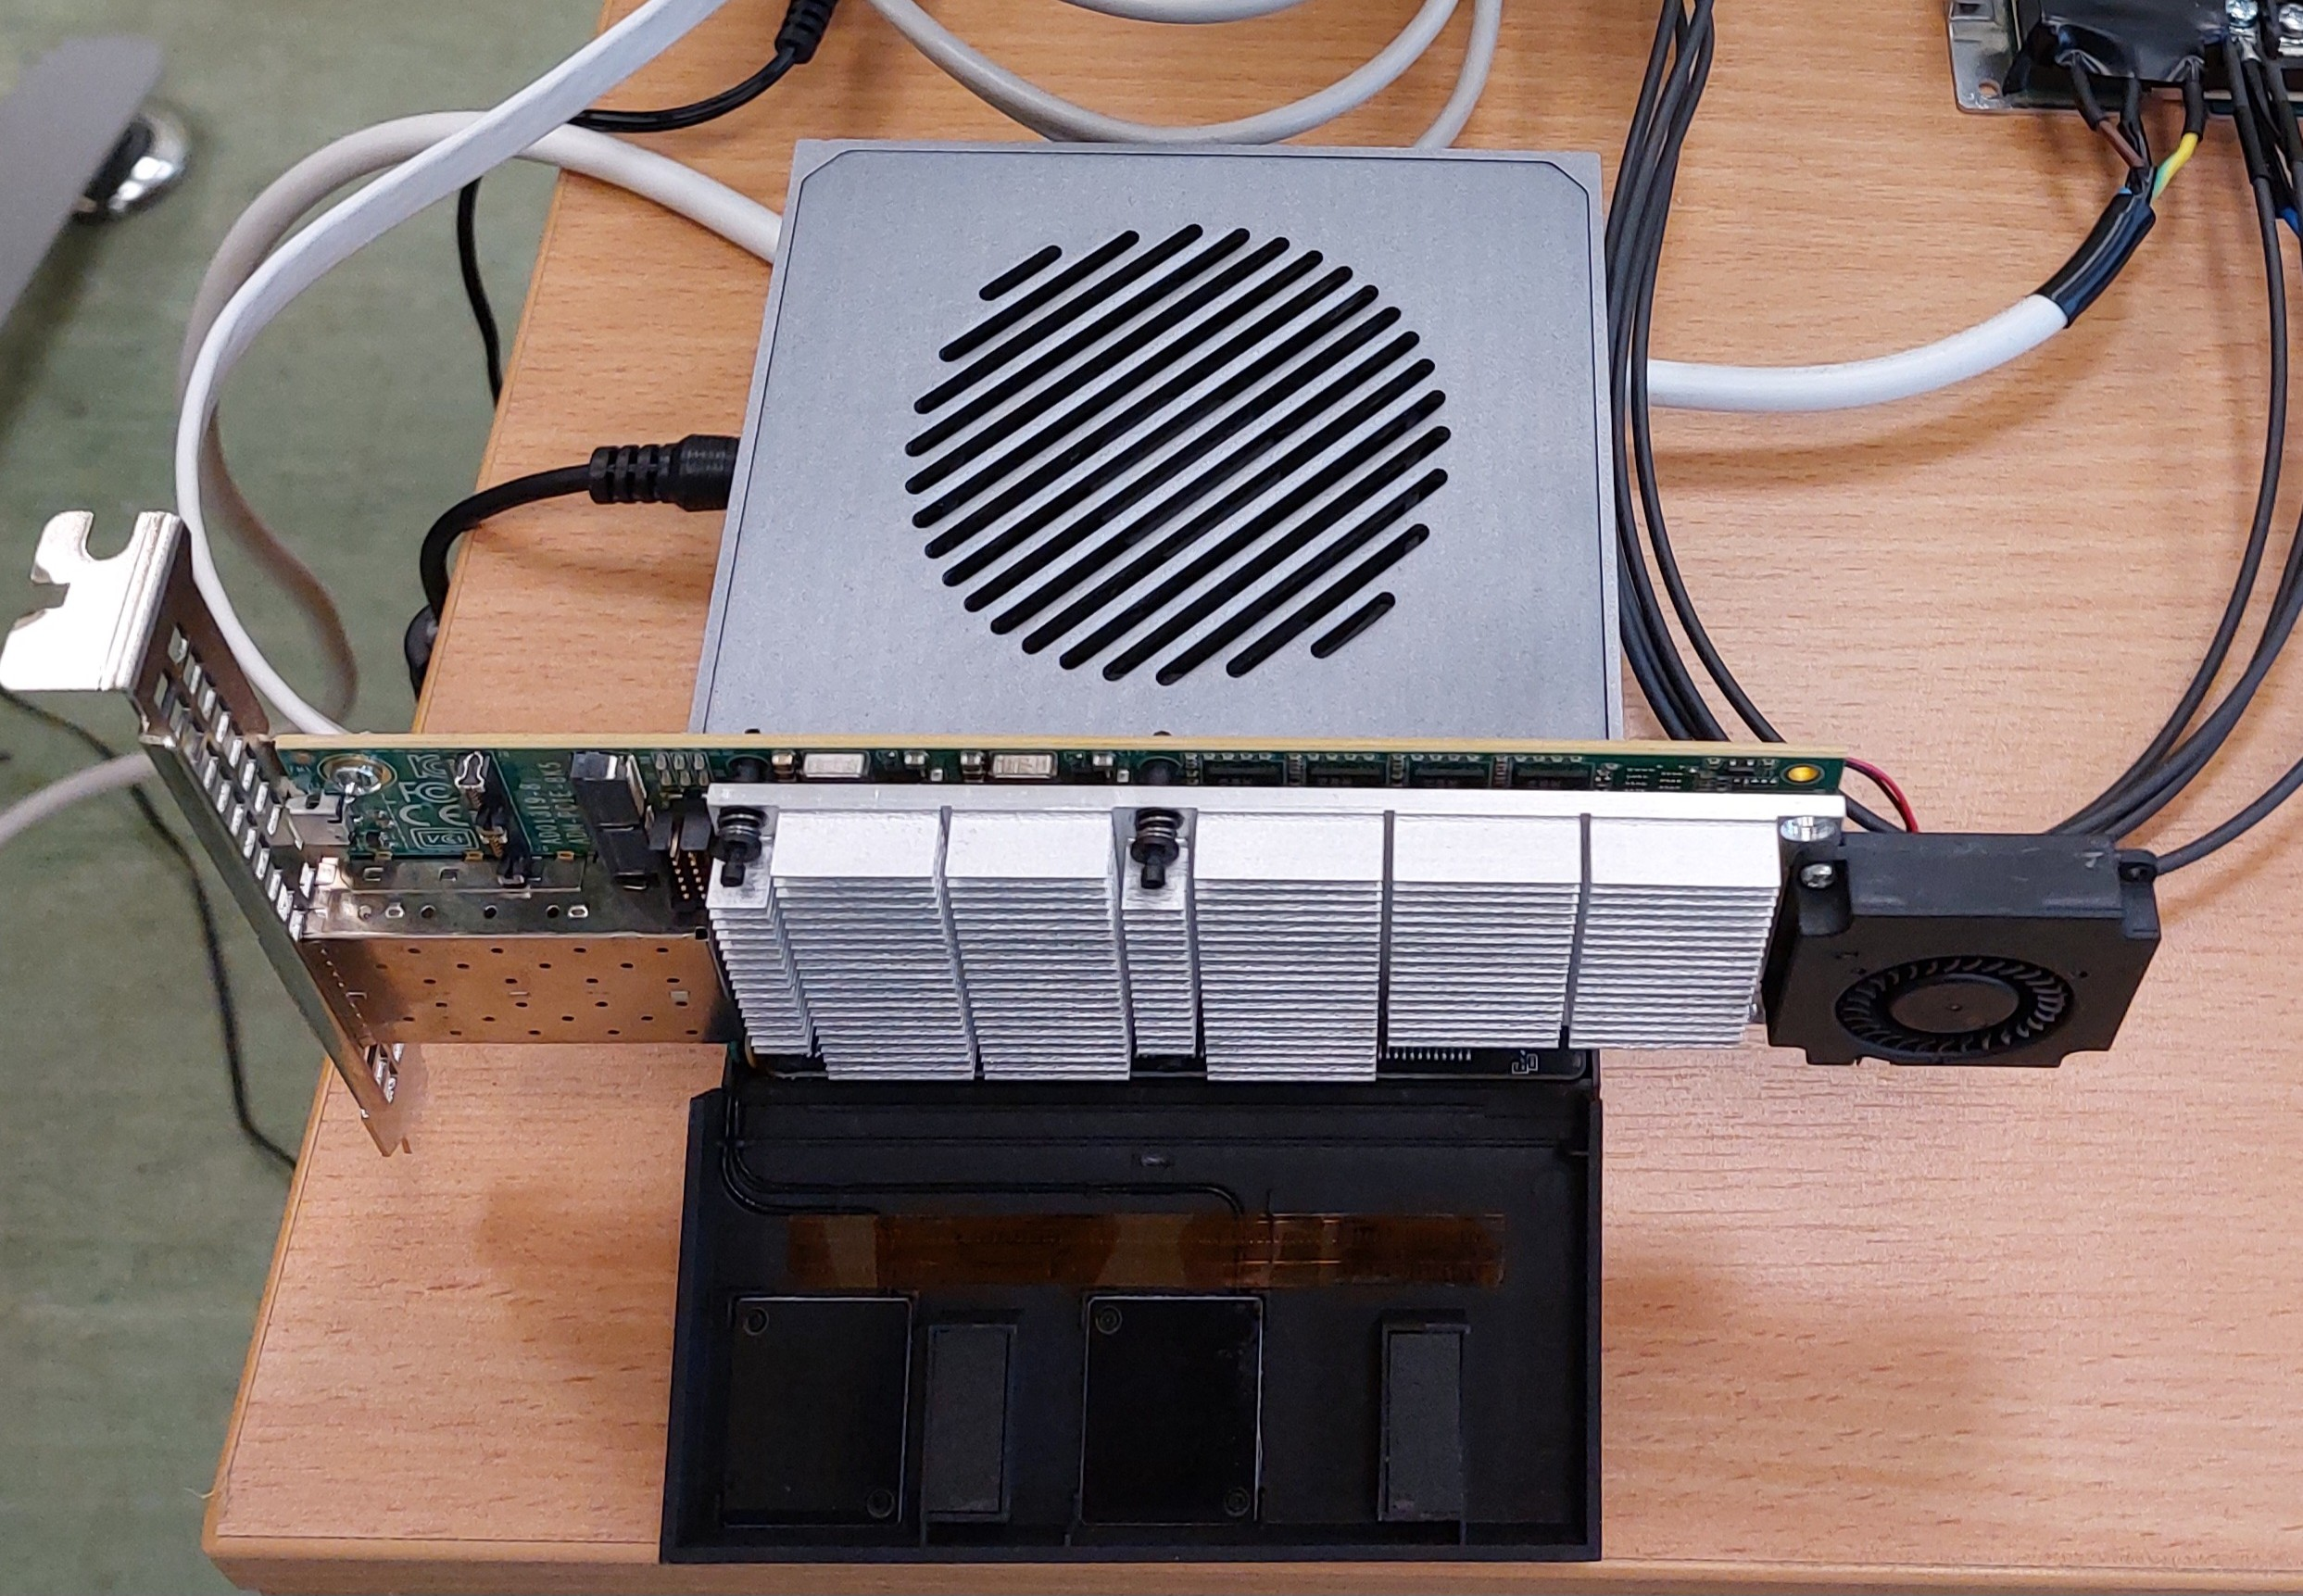
\includegraphics[width=0.8\linewidth]{fig/fpga_jetson.jpg}
\caption{Eksperimentālā novērtējuma platforma, kas sastāv no \textit{NVIDIA Jetson AGX Orin} sistēmas un \textit{Alpha Data ADM-PCIE-8K5} PCIe FPGA paātrinātāja kartes.}
\label{fig:fpga_jetson}
\end{figure}

Tādējādi platforma apvieno procesorā darbināmas programmatūras elastību ar \Gls{fpga} aparatūras uz notikumiem balstītu izpildi, nodrošinot vidi perifērijas mākslīgā intelekta lietojumiem paredzētu neiromorfo paātrinātāju pētniecībai.

Šī platforma ļauj realizēt \ref{fig:overall_arch}. attēlā parādīto straumēšanas paātrinātāju. Straumēšanas paātrinātājs
aprīkots ar AXI Stream saderīgām saskarnēm, savukārt PCIe \Gls{dma} modulis pārsūta konfigurāciju un datus starp
procesoru un \Gls{fpga} ierīci. Iegultajā sistēmā nodrošinātas programmatūras abstrakcijas kvantētu \Gls{snn} modeļu ielādei un
efektīvai impulsu datu apmaiņai \Gls{aer} reprezentācijā. Modeļa parametri, tostarp kvantētie konvolūcijas svari un nobīdes,
kā arī neironu slāņu konfigurācijas vērtības (solis, malu papildinājums, sliekšņi, laika konstantes), tiek pārsūtīti
paātrinātājam, izmantojot atmiņā kartētu piekļuvi pa PCIe saskarni. Šie parametri tiek ierakstīti mikroshēmas iekšējos
konfigurācijas reģistros un BRAM ar AXI-Lite transakcijām. Izpildes laikā laikā kodētās impulsu straumes starp procesoru
un paātrinātāju tiek apmainītas kā \Gls{aer} paketes \Gls{dma} straumēs. Šis ļauj ieviest kvantētus dziļos
\Gls{snn} modeļus un atvieglo integrāciju ar augstāka līmeņa ietvariem, piemēram, \textit{PyTorch} un \textit{SpikingJelly}.



    \paragraph{Salīdzinoša veiktspējas analīze}\mbox{} \\
  

Izmantojot \textit{SpikingJelly} ietvaru ar temporālu impulsu kodēšanu 4 laika soļos, apmācīti trīs konvolucionāli \Gls{snn} modeļi, lai novērtētu piedāvāto realizāciju dažādos tīkla mērogos. Pirmais ir kompakts divslāņu tīkls, kas apmācīts ar \textit{MNIST} datu kopu. Otrais un trešais ir dziļāki tīkli, kas apmācīti \textit{Caltech-101} attēlu klasifikācijas uzdevumam, izmantojot attiecīgi četrus un sešus konvolūcijas slāņus. Trīs tīklu arhitektūras ilustrētas \ref{fig:evaluation_networks}. attēlā.

Divslāņu \textit{MNIST} tīkls sastāv no konvolūcijas slāņiem ar 8 un 16 izejas kanāliem, izmantojot \(3\times3\) kodolus. Četrslāņu \textit{Caltech-101} tīkls sastāv no konvolūcijas slāņiem ar 8, 16, 32 un 64 izejas kanāliem, arī izmantojot \(3\times3\) kodolus. Sešslāņu \textit{Caltech-101} tīklam kanālu konfigurācija ir \(8, 16, 32, 32, 64, 64\) ar \(3\times3\) kodoliem. Starp izvēlētiem konvolūcijas slāņiem ievietoti apvienošanas slāņi ar \(2\times2\) logiem, lai samazinātu telpiskos izmērus.

Četrslāņu \textit{Caltech-101} tīkls apmācīts un novērtēts, izmantojot datu kopas pirmās piecas klases, savukārt sešslāņu
tīklam izmantotas pirmās desmit klases. Tas nodrošina divus arvien sarežģītākus klasifikācijas uzdevumus, vienlaikus
palielinot tīkla dziļumu. Šīs konfigurācijas ļauj novērtēt \Gls{fpga} realizācijas mērogojamību.

\begin{figure}[!t]
    \centering
    \begin{subfigure}{0.32\linewidth}
        \centering
        % 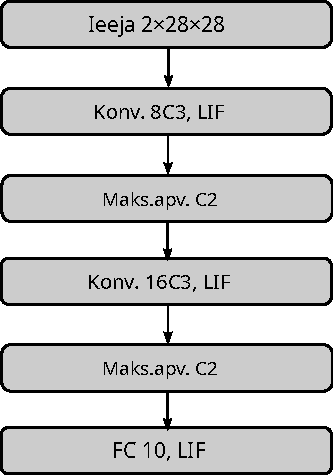
\includegraphics[width=\linewidth]{fig/lv/layer_structure_2.pdf}
        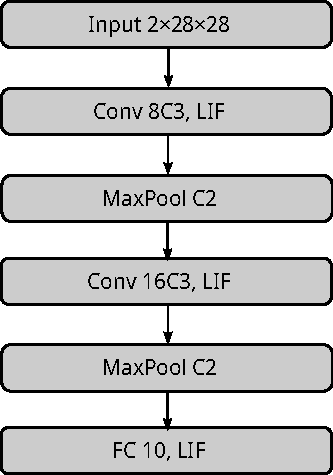
\includegraphics[width=\linewidth]{fig/layer_structure_2.pdf}
        \caption{MNIST, 2 slāņi.}
        \label{fig:layer_structure_2}
    \end{subfigure}
    \hfill
    \begin{subfigure}{0.32\linewidth}
        \centering
        % 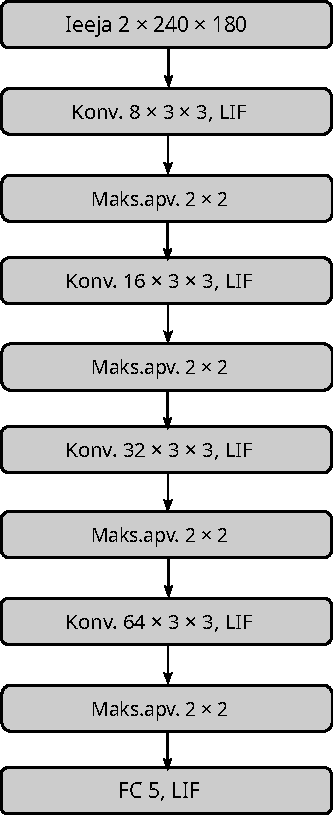
\includegraphics[width=\linewidth]{fig/lv/layer_structure_4.pdf}
        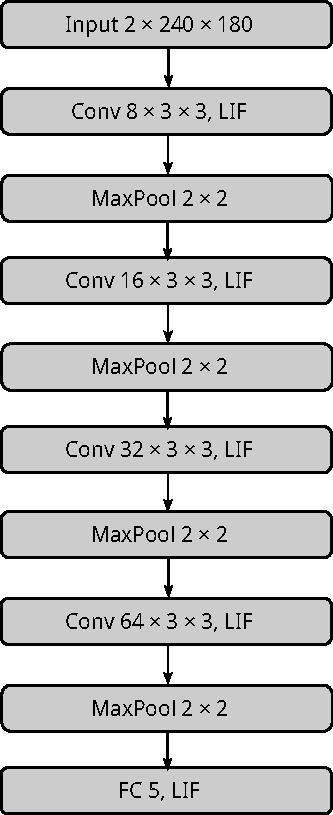
\includegraphics[width=\linewidth]{fig/layer_structure_4.pdf}
        \caption{Caltech-101, 4 slāņi.}
        \label{fig:layer_structure_4}
    \end{subfigure}
    \hfill
    \begin{subfigure}{0.32\linewidth}
        \centering
        % 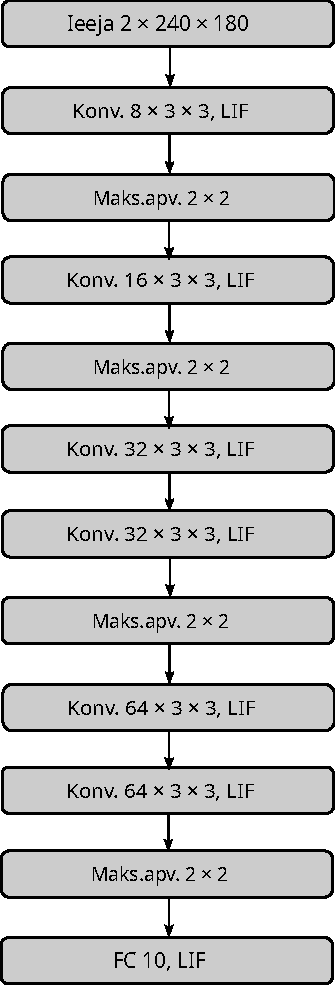
\includegraphics[width=\linewidth]{fig/lv/layer_structure_6.pdf}
        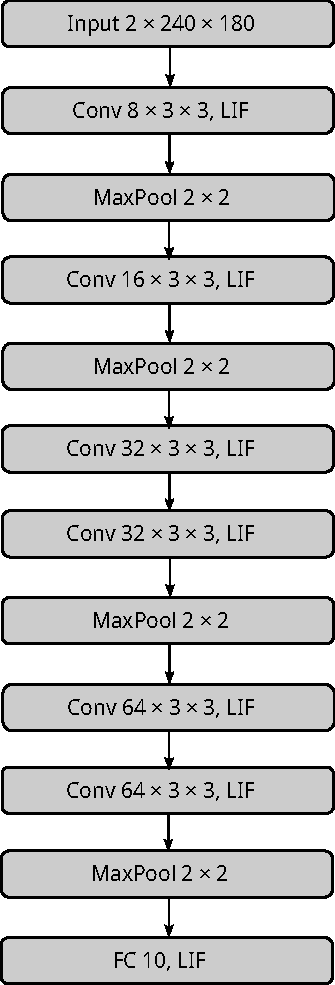
\includegraphics[width=\linewidth]{fig/layer_structure_6.pdf}
        \caption{Caltech-101, 6 slāņi.}
        \label{fig:layer_structure_6}
    \end{subfigure}
    \caption{Eksperimentālajā novērtējumā izmantotās SNN arhitektūras:
    (\subref{fig:layer_structure_2}) divslāņu MNIST tīkls,
    (\subref{fig:layer_structure_4}) četrslāņu Caltech-101 tīkls un
    (\subref{fig:layer_structure_6}) sešslāņu Caltech-101 tīkls.}
    \label{fig:evaluation_networks}
\end{figure}

Apmācības laikā pēc konvolūcijas slāņiem ievietoti pakešu normalizācijas slāņi, lai uzlabotu optimizāciju un apmācības stabilitāti. Inferences laikā pakešu normalizācija tiek apvienota ar konvolūcijas svariem un nobīdēm. Tādēļ pakešu normalizācijai nav nepieciešams atsevišķs aparatūras slānis un tā nav parādīta \ref{fig:evaluation_networks}. attēlā.

Svariem piemērota \Gls{ptq} ar dažādiem bitu platumiem, lai novērtētu tās ietekmi uz klasifikācijas veiktspēju. Kā parādīts
\ref{tab:quant_compare}. tabulā, abiem modeļiem F1 rādītājs samazinās tikai nedaudz līdz pat 4 bitu precizitātei, savukārt,
samazinot bitu platumu zem 4 bitiem, veiktspēja kļūst nestabila. F1 rādītāja atšķirības saglabājās 1~\% robežās attiecībā
pret 32 bitu atskaites vērtību. Samazinot sešslāņu tīkla svaru precizitāti līdz 2 bitiem, F1 rādītājs ievērojami samazinājās līdz
41,98~\%, norādot, ka jutība pret kvantēšanu ir atkarīga no tīkla dziļuma.

\begin{table}
\centering
\caption{Kvantēšanas ietekme uz SNN arhitektūru inferences F1 rādītāju}
\label{tab:quant_compare}
\begin{tabular}{@{}lccccc@{}}
\toprule
\textbf{Kvantēšana}       & \textbf{32 biti} & \textbf{16 biti} & \textbf{8 biti} & \textbf{4 biti} & \textbf{2 biti}    \\ \midrule
\multicolumn{6}{c}{28\texttimes 28-8C3-P2-16C3-P2} \\
\midrule
F1 rādītājs MNIST [\%]        & 96{,}78   & 96{,}80   & 96{,}81   & 96{,}79   & 90{,}10   \\
\midrule
\multicolumn{6}{c}{240\texttimes 180-8C3-P2-16C3-P2-32C3-P2-64C3-P2} \\
\midrule
F1 rādītājs Caltech-101 [\%]  & 88{,}87   & 88{,}67   & 89{,}07   & 89{,}32   & 87{,}19   \\
\midrule
\multicolumn{6}{c}{240\texttimes 180-8C3-P2-16C3-P2-32C3-32C3-P2-64C3-64C3-P2} \\
\midrule
F1 rādītājs Caltech-101 [\%]  & 87{,}99 & 87{,}37  & 86{,}85  &  88{,}10  & 41{,}98 \\
\bottomrule
\end{tabular}
\end{table}

Inferences latentuma salīdzināšanai kvantētie \Gls{snn} modeļi izpildīti \textit{NVIDIA GeForce RTX 5070 Ti}, \textit{NVIDIA Jetson AGX Orin} un \textit{Kintex UltraScale KU115-2} \Gls{fpga} platformās. Salīdzinājums ietvēra divslāņu \textit{MNIST} modeli un četrslāņu un sešslāņu \textit{Caltech-101} modeļus. \ref{tab:execution_time}. tabulā parādīti katrai platformai izmērītie apstrādes laiki, datu pārsūtīšanas laiki un kopējie inferences latentumi. \Gls{fpga} sasniedza attiecīgi \qty{1.10}{\milli\second}, \qty{2.43}{\milli\second} un \qty{2.81}{\milli\second} kopējo latentumu trim tīkliem. Salīdzinājumā ar \textit{Jetson AGX Orin} šie rezultāti parāda latentuma samazinājumu attiecīgi par \qty{2.30}{\milli\second}, \qty{2.35}{\milli\second} un \qty{3.60}{\milli\second}. \textit{RTX 5070 Ti} visiem trim tīkliem sasniedza mazāku kopējo latentumu nekā \Gls{fpga}, ar atšķirību attiecīgi \qty{0.30}{\milli\second}, \qty{1.28}{\milli\second} un \qty{1.66}{\milli\second}. Šie rezultāti demonstrē, ka piedāvātais \Gls{fpga} paātrinātājs nodrošina mazāku inferences latentumu nekā iegultā GPU platforma, lai gan augstas veiktspējas diskrētais GPU pārbaudītajiem tīkliem joprojām ir ātrāks.

\begin{table}[t]
\centering
\caption{Inferences latentums FPGA un GPU aparatūras platformām, izmantojot tīklus ar 2 un 4 konvolūcijas slāņiem
}
\label{tab:execution_time}
\begin{tabular}{lcccc}
\toprule
\textbf{Ierīce} & \textbf{Sinhr. uz} & \textbf{Apstrāde} & \textbf{Sinhr. no} & \textbf{Kopā} \\
 & \textbf{ierīci (ms)} & \textbf{(ms)} & \textbf{ierīces (ms)} & \textbf{(ms)} \\
\midrule
\multicolumn{5}{c}{28\texttimes 28-8C3-P2-16C3-P2} \\
\midrule
RTX5070 Ti & 0{,}05 & 0{,}70 & 0{,}05 & 0{,}80 \\
UltraScale KU115-2 & 0{,}08 & 0{,}95 & 0{,}08 & 1{,}10 \\
Jetson AGX Orin & 0{,}75 & 2{,}10 & 0{,}55 & 3{,}40 \\
\midrule
\multicolumn{5}{c}{240\texttimes 180-8C3-P2-16C3-P2-32C3-P2-64C3-P2} \\
\midrule
RTX5070 Ti & 0{,}06 & 1{,}00 & 0{,}06 & 1{,}12 \\
UltraScale KU115-2 & 0{,}09 & 2{,}25 & 0{,}09 & 2{,}43 \\
Jetson AGX Orin & 0{,}90 & 3{,}15 & 0{,}70 & 4{,}75 \\
\midrule
\multicolumn{5}{c}{240\texttimes 180-8C3-P2-16C3-P2-32C3-32C3-P2-64C3-64C3-P2} \\
\midrule
RTX5070 Ti & 0{,}07 & 1{,}02 & 0{,}06 & 1{,}15 \\
UltraScale KU115-2 & 0{,}09 & 2{,}64 & 0{,}08 & 2{,}81 \\
Jetson AGX Orin & 0{,}94 & 4{,}87 & 0{,}60 & 6{,}41 \\
\bottomrule
\end{tabular}
\end{table}

\ref{tab:sparsity}. tabulā piedāvātais paātrinātājs salīdzināts ar esošām uz \Gls{fpga} balstītām konvolucionālo \Gls{snn} realizācijām. Lai gan esošie darbi galvenokārt orientēti uz sekliem tīkliem un vienkāršākām datu kopām, piemēram, \textit{MNIST}, piedāvātais risinājums atbalsta dziļākas arhitektūras un augstākas izšķirtspējas datu kopas (piemēram, \textit{Caltech-101}), saglabājot konkurētspējīgu caurlaidību un mērenu resursu izmantojumu.

\begin{table}[t]
\centering
\footnotesize
\vspace{0.05in}
\caption{Uz FPGA balstītu CSNN realizāciju salīdzinājums iepriekšējos darbos un šajā darbā}
\label{tab:sparsity}
\begin{adjustbox}{max width=\textwidth}
  \begin{tabular}{@{}lp{1.7cm}p{1.7cm}p{1.7cm}p{1.7cm}p{1.6cm}p{1.6cm}p{1.6cm}@{}}
\toprule
\textbf{Darbs}       & \textbf{Sommer u.\,c.} \cite{sommer2022} & \textbf{Plagwitz u.\,c.} \cite{plagwitz2025} & \textbf{Zhang
    u.\,c. \cite{zhang2024b}} & \textbf{Zhang u.\,c. \cite{zhang2024b}} & \textbf{Šis darbs} & \textbf{Šis darbs} & \textbf{Šis darbs} \\ \midrule
Platforma            & XCZU7EV & XCZU9EG     & XC7Z020     & XC7Z020     & KU115-2 & KU115-2 & KU115-2 \\
Arhitektūra        & 3CL-1PL-1FC & 4CL-4PL-2FC & 2CL-2PL-1FC & 2CL-2PL & 2CL-2PL & 4CL-4PL & 6CL-6PL \\
Datu kopa             & MNIST & CIFAR-10    & MNIST       & Caltech-101 & MNIST   & Caltech-101 & Caltech-101 \\
\textbf{\(H \times W\)} & \(28 \times 28\) & \(32 \times 32\) & \(28 \times 28\) & \(240 \times 180\) & \(28 \times 28\) & \(240 \times 180\) & \(240 \times 180\) \\
\midrule
Resursi [LUTs]    & 19\,000 & 49\,930 & 628 & 1\,207 & 15\,627 & 41\,150 & 64\,687 \\
Resursi [FFs]     & 12\,000 & 28\,739 & -   & 1\,460 & 18\,671 & 59\,215 & 77\,122 \\
Resursi [BRAM]    & 2{,}1 Mib & 1{,}93 Mib & - & 1{,}25 Mib & 1{,}84 Mib  & 4{,}42 Mib & 5{,}07 Mib \\
Resursi [DSPs]    & 32     & 0      & -   & 0      & 0    & 0       & 0       \\
Kvantēšana [biti] & 8     & 4      & 2   & 2     & 8      & 8      & 8      \\
\bottomrule
\end{tabular}
\end{adjustbox}
\end{table}

\Gls{fpga} arhitektūras uzlaboto mērogojamību nodrošina hibrīda atmiņas organizācija, kurā sinaptiskie svari, dažādi \Gls{fifo}, \Gls{dma} buferi un starpsavienojumu buferi realizēti ar mikroshēmas iekšējo \Gls{bram}, savukārt membrānas potenciāli glabāti ārējā atmiņā un straumēti inferences laikā. Tādēļ tā paša tīkla realizācijai ar visiem membrānas potenciāliem mikroshēmā būtu nepieciešama papildu \Gls{bram} ietilpība.

Membrānas potenciālu atmiņas nepieciešamo apjomu tīklam ar \(L\) slāņiem aprēķina šādi:
\begin{equation}
  M_{\mathrm{memb}} = \sum_{l=1}^{L} C_l \times H_l \times W_l \times b_v,
\end{equation}
kur \(C_l\), \(H_l\) un \(W_l\) apzīmē attiecīgi membrānas potenciāla tenzora izejas kanālu skaitu, augstumu un platumu slānī
\(l\), un \(b_v=8\) biti ir šajā realizācijā izmantotā membrānas potenciāla precizitāte. Iegūtās glabāšanas prasības
novērtētajām tīklu konfigurācijām apkopotas \ref{tab:mp_resources}. tabulā.

Redzams, ka salīdzinājumā ar divslāņu \textit{MNIST} modeli četrslāņu un sešslāņu modeļi patērē ievērojami vairāk atmiņas, jo membrānas potenciālu apjoms pieaug līdz ar telpiskajiem izmēriem un dziļumu. Salīdzinājumā ar četrslāņu \textit{Caltech-101} tīklu sešslāņu konfigurācijai nepieciešams aptuveni par 19,9~\% vairāk membrānas potenciālu glabāšanas vietas.

\begin{table}[t]
\centering
\caption{Mikroshēmas iekšējās atmiņas prasības pilnībā iekšējai glabāšanai (svari un membrānas potenciāli iekšējā BRAM) un hibrīdai glabāšanai (membrānas potenciāli ārējā SDRAM un svari iekšējā BRAM)}
\label{tab:mp_resources}
\begin{tabular}{lcccc}
\toprule
  \textbf{Arhitektūra} & \textbf{Ārējā} & \textbf{Visa mikroshēmā} & \textbf{Samazinājums}\\
\midrule
  28\texttimes 28-2CL-2PL   & 73{,}50Kib & 1{,}91Mib  & 3{,}8~\% \\
  240\texttimes 180-4CL-4PL & 4{,}93Mib  & 9{,}35Mib  & 52{,}8~\% \\
  240\texttimes 180-6CL-6PL & 5{,}91Mib  & 10{,}98Mib & 53{,}9~\% \\
\bottomrule
\end{tabular}
\end{table}

„Hibrīda” realizācijas \Gls{bram} izmantojums, kas norādīts \ref{tab:sparsity}. tabulā, jau ietver svariem, dažādiem
\Gls{fifo} buferiem un starpsavienojumu buferēšanai piešķirto mikroshēmas iekšējo atmiņu, bet neietver membrānas potenciālu
glabāšanu. Lai novērtētu papildu \Gls{bram} ietilpību teorētiskai pilnībā mikroshēmā izvietotai realizācijai, membrānas
potenciālu atmiņu var pieskaitīt nepieciešamajai svaru atmiņai. Tādējādi idealizēto \Gls{bram} daudzumu pilnībā mikroshēmā
izvietotai alternatīvai var izteikt kā
\begin{equation}
  M_{\mathrm{all\mbox{-}on\mbox{-}chip}}
  \approx M_{\mathrm{hybrid}} + M_{\mathrm{memb}},
\end{equation}
kur \(M_{\mathrm{hybrid}}\) apzīmē esošās hibrīda realizācijas aizņemto \Gls{bram} ietilpību (\ref{tab:sparsity}. tabula).
Relatīvo mikroshēmas iekšējās atmiņas nepieciešamo daudzuma samazinājumu, kas panākts, membrānas potenciālus glabājot ārēji, aprēķina šādi:
\begin{equation}
  R =
  \frac{M_{\mathrm{all\mbox{-}on\mbox{-}chip}} - M_{\mathrm{hybrid}}}
       {M_{\mathrm{all\mbox{-}on\mbox{-}chip}}}
  \times 100~\%.
\end{equation}
Kā parādīts \ref{tab:mp_resources}. tabulā, hibrīda atmiņas arhitektūra samazina teorētiskās mikroshēmas iekšējās atmiņas
prasības attiecīgi par 52,8~\% un 53,9~\% četrslāņu un sešslāņu \textit{Caltech-101} tīkliem. Redzams arī, ka hibrīda atmiņas
arhitektūras ieguvums ir atkarīgs no tīkla arhitektūras un membrānas potenciālu glabāšanas relatīvā ieguldījuma kopējā
iekšējā atmiņā. Divslāņu \textit{MNIST} tīklam membrānas potenciālu ārēja glabāšana samazina iekšējo atmiņu tikai par 3,8~\%,
jo membrānas potenciālu glabāšana veido samērā mazu daļu no kopējā atmiņas apjoma, savukārt četrslāņu un sešslāņu
arhitektūrām ir būtiski lielākas starpposmu pazīmju kartes un ar tām saistītā membrānas potenciālu atmiņa. Tas norāda, ka
mazāku pazīmju karšu gadījumā dominē citas atmiņas sastāvdaļas un membrānas potenciālu vērtības varētu glabāt pilnībā
mikroshēmā.

\ref{tab:power_usage}. tabulā parādīts vienas inferences enerģijas patēriņš četrslāņu \textit{Caltech-101} \Gls{snn} un
\Gls{ann} realizācijām. \Gls{snn} demonstrē būtiski mazāku enerģiju nekā \Gls{ann} pat vairākiem laika soļiem, galvenokārt
pateicoties retiem impulsu aprēķiniem un svaru glabāšanai mikroshēmas iekšējā BRAM. Tomēr stāvokļu atmiņas enerģija veido ievērojamu daļu no kopējās \Gls{snn} jaudas. Lai gan sinaptisko operāciju skaits \(N_{SynOp}\) ir daudz lielāks nekā neironu skaits \(N_{Neurons}\), atmiņas piekļuves enerģija saglabājas augsta ārpusmikroshēmas piekļuves lielo izmaksu dēļ, t.\,i., \(E_{SDRAM} >> E_{BRAM}\). Ieejas gadījums \(1 \times 2\) ir energoefektīvākais, aptuveni atbilstot \Gls{ttfs} konfigurācijai, kur membrānas potenciāli tiek atjaunināti tikai līdz pirmā impulsa rašanās brīdim.

Tomēr \Gls{ann} enerģijā dominē DRAM piekļuves svariem un aktivācijām, un int8 kvantēšana dod tikai nelielu ietaupījumu,
uzsverot \Gls{snn} impulsu retuma priekšrocības.

Lai gan analītiskais novērtējums nodrošina algoritmisko enerģijas priekšrocību atskaites vērtību, papildu tiek norādīts
\textit{Xilinx Power Analyzer} ziņotais patēriņš, ar kuru saskaņā kopējais dinamiskais jaudas patēriņš mikroshēmā ir 0,45~W. Atšķirība starp
izmērīto kopējo jaudu un analītisko novērtējumu tiek skaidrota ar kopējo mikroshēmas jaudu, tostarp takts signāla sadales
koku un PCIe DMA infrastruktūru. Neraugoties uz to, kopējā jauda saglabājas būtiski mazāka nekā augstas veiktspējas GPU
risinājumiem.

\begin{table}[h!]
\centering
\caption{Vienas inferences enerģijas patēriņš četrslāņu Caltech-101 SNN un ANN modeļiem, sadalot kopējo enerģiju sinaptisko operāciju un membrānas stāvokļu ieguldījumos}
\label{tab:power_usage}
\begin{tabular}{@{}lccccc@{}}
\toprule
\textbf{Modelis} & \textbf{\(T\times D\)} & \textbf{Kopējā enerģija (\unit{\micro\joule})} & \textbf{Sin./mem. enerģija (\unit{\micro\joule})}  \\ \midrule
SNN [int8]  & \(1 \times 2\)   & 120{,}201   & 64{,}290  / 55{,}910   \\
SNN [int8]  & \(4 \times 2\)   & 480{,}805   & 257{,}163 / 223{,}641  \\
ANN [int8]  & \(1 \times 1\)   & 414{,}719   &  -  \\
ANN [fl32]  & \(1 \times 1\)   & 466{,}624   &  -  \\
\bottomrule
\end{tabular}
\end{table}

Papildus jaudas mērījumi veikti tieši \textit{Alpha Data ADM-PCIE-8K5} paātrinātāja kartē inferences laikā. Kartē ir
sprieguma un strāvas sensori, kuru nolasījumi iegūti ar mikrokontrollera lietojumrīku. Jaudas rādījumi 12~V barošanas ķēdē
nepārtraukti reģistrēti 10\,000 paraugu intervālā dīkstāvē un aktīvas inferences laikā četrslāņu \textit{Caltech-101} tīklam
($T\times D = 4\times 2$). \ref{tab:measured_power_stats}. tabulā norādītās jaudas vērtības ir reģistrēto paraugu vidējā
vērtība un standartnovirze.

Dīkstāvē kartes vidējais kopējais jaudas patēriņš bija $15{,}771 \pm 0{,}069\,\text{W}$. Inferences laikā vidējais jaudas patēriņš pieauga līdz $15{,}862 \pm 0{,}070\,\text{W}$. Lai atšķirtu inferences papildu jaudu no platformas dīkstāves jaudas, izmērīto dinamisko jaudas patēriņu definē šādi:
\begin{equation}
    P_{\mathrm{dyn}} =
    P_{\mathrm{inference}} - P_{\mathrm{idle}}.
\end{equation}
Papildu enerģija vienai inferencei novērtēta, kopējās platformas jaudas vietā izmantojot \(P_{\mathrm{dyn}}\). Starpība starp izmērītajām vidējām vērtībām norāda uz aptuveni $91\,\text{mW}$ paātrinātāja jaudas patēriņu. Testa laikā vidējais vienas inferences ilgums bija \qty{2.4}{\milli\second}, un vienas inferences enerģija bija 218,4~$\mu$J. Nelielais dinamiskās jaudas pieaugums apstiprina, ka kopējā patēriņā dominē PCIe kartes statiskā jauda, savukārt uz notikumiem balstītais \Gls{snn} kodols veic energoefektīvus aprēķinus.

\begin{table}[htbp]
\centering
\caption{ADM-PCIE-8K5 FPGA paātrinātāja kartes jaudas un enerģijas mērījumi dīkstāvē un aktīvas inferences laikā ($T\times D = 4\times 2$, četrslāņu Caltech-101 modelis, 10\,000 paraugu)}
\label{tab:measured_power_stats}
\begin{tabular}{l r r}
\toprule
\textbf{Metrika} & \textbf{Dīkstāve} & \textbf{Inference} \\
\midrule
Vidējā jauda & 15{,}771 $\pm$ 0{,}069 W & 15{,}862 $\pm$ 0{,}070 W \\
Min./maks. jauda & 15{,}572 / 15{,}975 W & 15{,}722 / 16{,}055 W \\
Inferences jauda & -- & 91 mW \\
Vidējais inferences laiks & -- & \qty{2.4}{\milli\second} \\
Vienas inferences enerģija & -- &  218{,}4 $\mu$J \\
\bottomrule
\end{tabular}
\end{table}



  \subsubsection{Telpiski temporāla objektu detektēšana ar dziļiem impulsu CNN, izmantojot LiDAR datus}
    \paragraph{Eksperimentu konfigurācija}\mbox{} \\
    Objektu detektēšanas tīkls, kas sastāv no impulsu \textit{VGG} pamattīkla un tam sekojošas \Gls{ssd} galvas, parādīts \ref{fig:spiking_vgg_ssd}. attēlā. \textit{VGG} pamattīkls iegūst pazīmes no \Gls{tvc} reprezentācijas, savukārt \Gls{ssd} detektēšanas galva no iegūtajām pazīmju kartēm prognozē objektu klases un ietverošo taisnstūru parametrus. Lai izpētītu tīkla dziļuma ietekmi uz detektēšanas precizitāti un aprēķinu izmaksām, novērtētas divas konfigurācijas, kuru pamatā ir \textit{VGG-11} un \textit{VGG-13}.

Tīkls apmācīts un novērtēts ar \textit{KITTI} objektu detektēšanas datu kopu \cite{geiger2012}. Detektēšanas veiktspēja novērtēta atbilstoši \textit{KITTI} \Gls{bev} novērtēšanas protokolam, izmantojot pagrieztu taisnstūru \Gls{iou} slieksni 0,7 automobiļu klasei un 0,5 gājēju un velosipēdistu klasēm. Vidējā precizitāte aprēķināta 40 pilnīguma pozīcijās \(AP_{R40}\) vieglajam, vidējam un sarežģītajam grūtības līmenim. Pieejamie apmācības dati sadalīti 80~\% apmācības un 20~\% validācijas apakškopās. Novērtēšana veikta \Gls{bev} ietverošajiem taisnstūriem, savukārt vizualizācijai 3D ietverošie paralēlskaldņi rekonstruēti, piešķirot statistiski novērtētus objektu augstumus. Detektēšanas rezultātu piemēri parādīti \ref{fig:3D_detections}. attēlā.

\begin{figure}[t]
    \centering
    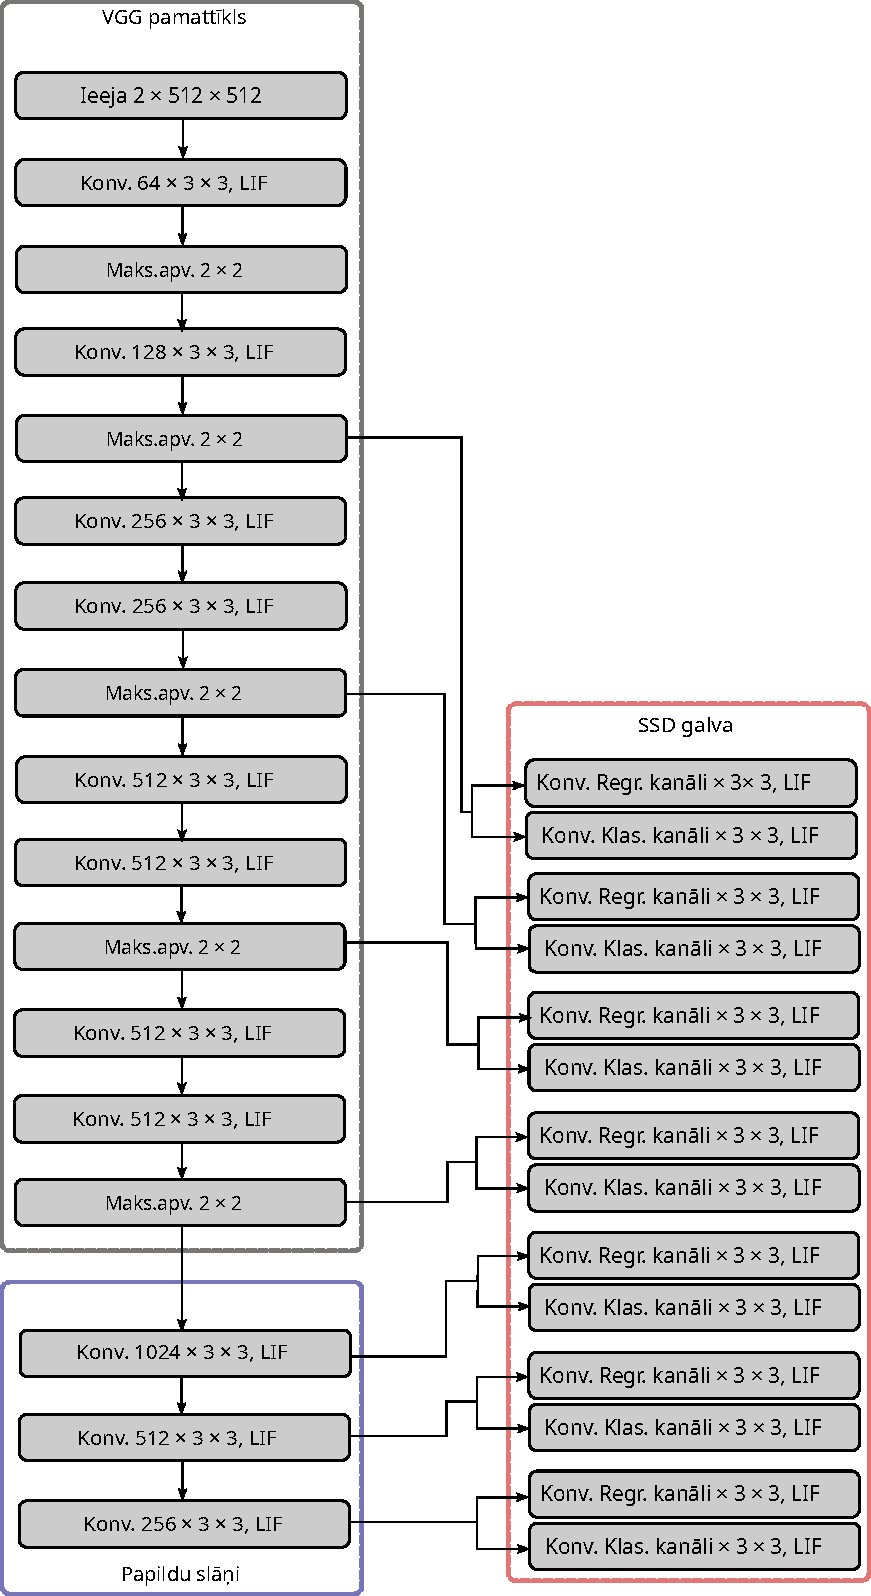
\includegraphics[width=0.5\textwidth]{fig/lv/spiking_vgg_ssd.pdf}
    \caption{Impulsu VGG pamattīkls un viena posma SSD detektēšanas galva, kas izmantoti 3D objektu detektēšanai no TVC reprezentācijām.}
    \label{fig:spiking_vgg_ssd}
\end{figure}

\begin{figure}[t]
  \centerline{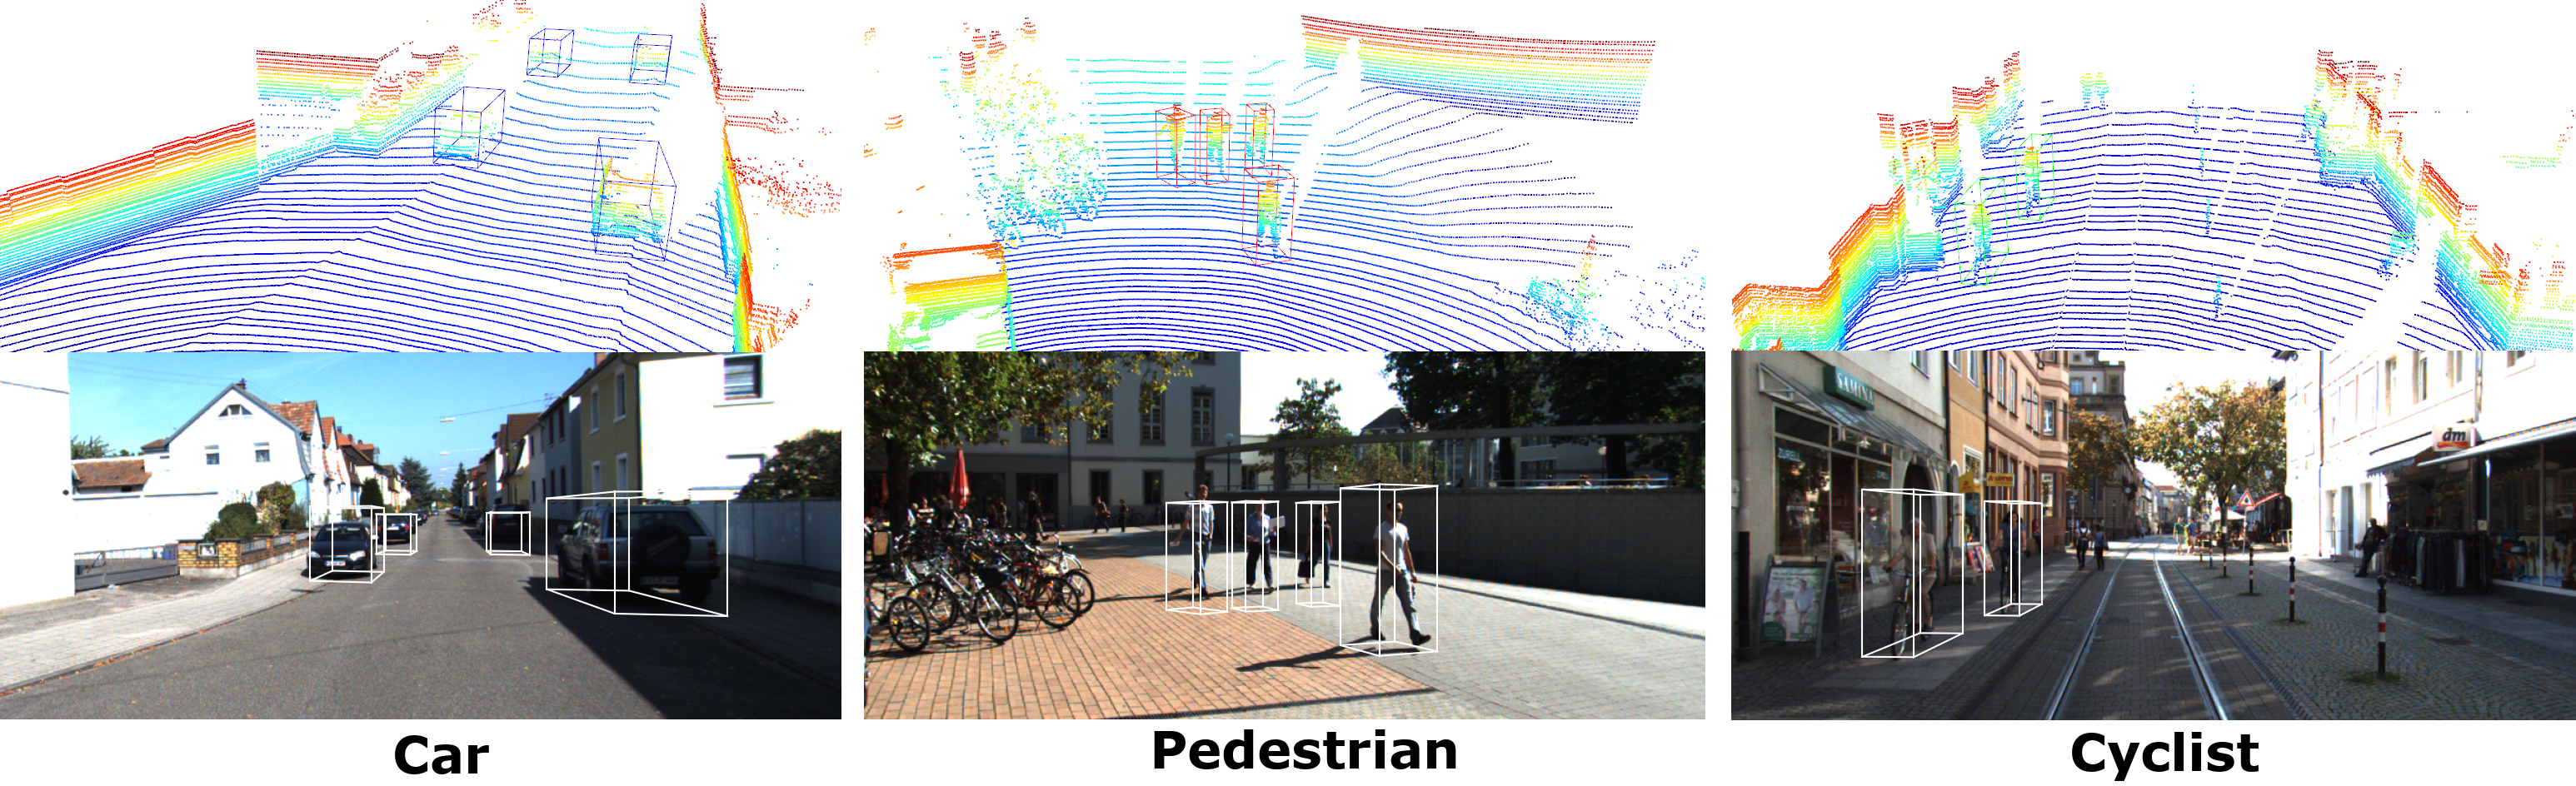
\includegraphics[width=\textwidth]{fig/7129.png}}
  \caption{3D ietverošo paralēlskaldņu detektēšanas rezultātu vizualizācija uz KITTI validācijas datu kopas attēliem.}
  \label{fig:3D_detections}
\end{figure}

Ieejas priekšapstrāde veikta, ņemot vērā ainas robežas \qtyrange{0}{50}{\metre} X asij, \qtyrange{-25}{25}{\metre} Y asij un \qtyrange{-2}{1}{\metre} Z asij, vienlaikus pētot izvēlētu vokselizācijas izmēru \([VS_x, VS_y, VS_z]\) diapazonu. Šeit \([VS_x, VS_y]\) nosaka katra \Gls{bev} šķēluma izšķirtspēju, savukārt \(VS_z\) nosaka laika soļu skaitu. \(VS_z\) iestatīts uz \qty{0.6}{\metre}, vienādi sadalot 3~m vertikālo diapazonu 5 \Gls{bev} šķēlumos un ļaujot izmantot dažādus \(t_{bin}\) izmērus, lai katrā šķēlumā iegūtu vairāk kanālu \(C\).

Abi modeļi, \textit{VGG-11} un \textit{VGG-13}, novērtēti vienādos apmācības apstākļos. Tādēļ eksperimenti ļauj analizēt vokseļu izšķirtspējas, pamattīkla dziļuma, impulsu retinājuma un parametru skaita ietekmi uz detektēšanas precizitāti.



    \paragraph{Salīdzinoša veiktspējas analīze}\mbox{} \\
  

\begin{figure}[t]
  \centerline{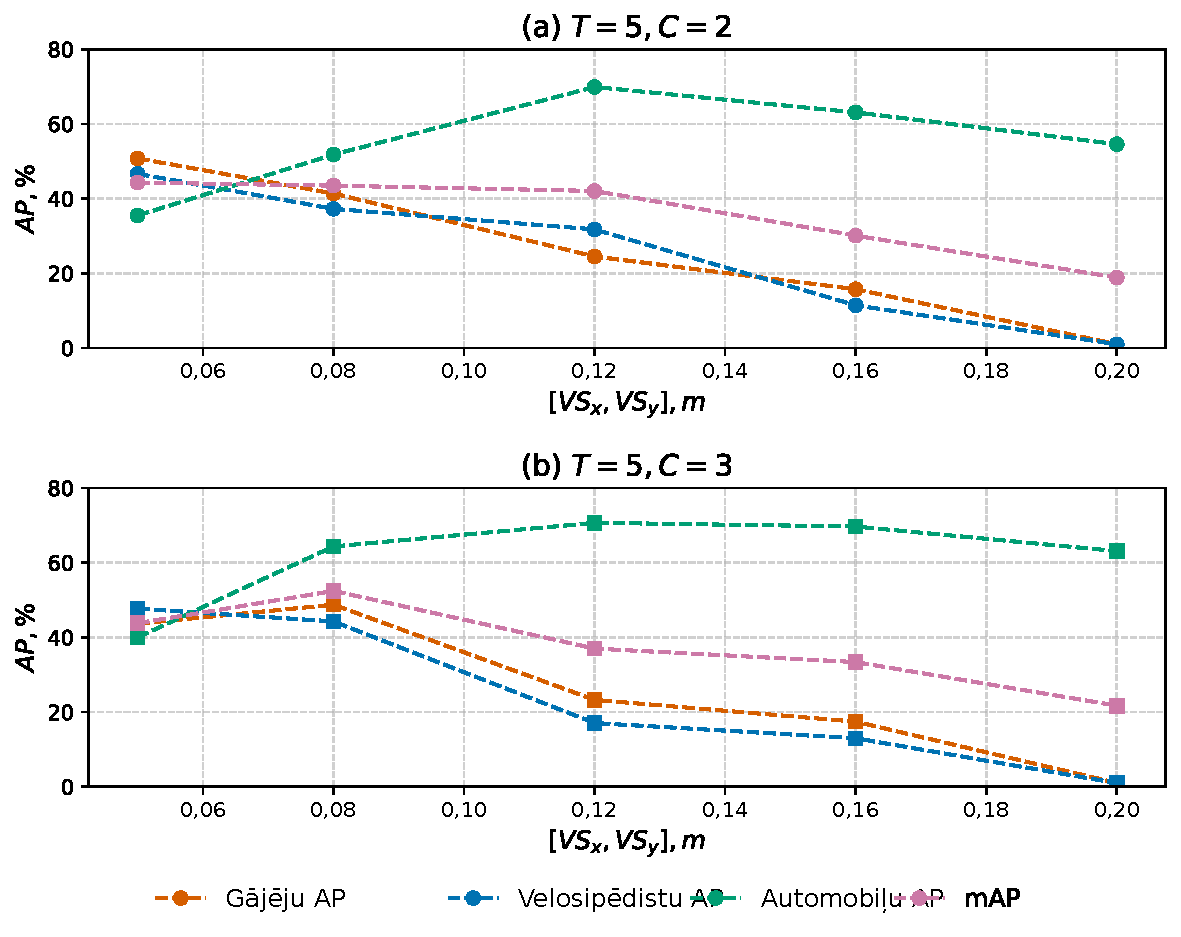
\includegraphics[width=0.75\textwidth]{fig/lv/voxel_size_chart_pretty.pdf}}
  \caption{Vokseļa izmēra ietekme uz vidējo precizitāti (AP), izmantojot impulsu VGG-11 pamattīklu ar (a) \(T=5\) laika soļiem un \(C=2\) kanāliem katrā laika solī; (b) \(T=5\) laika soļiem un \(C=3\) kanāliem katrā laika solī.}
  \label{fig:vox_size}
\end{figure}

\begin{table}[b]
\centering
\caption{Parametru skaita, retinājuma un vidējās precizitātes (\%) salīdzinājums dažādiem modeļiem}
\label{tab:detection_sparsity}
\footnotesize
\begin{adjustbox}{max width=\textwidth}\begin{tabular}{@{}lccccc@{}}
\toprule
Metode         & Param. sk. & Retinājums & Automobilis   & Gājējs & Velosipēdists \\ \midrule
Zhou u.\,c. \cite{Zhou2020} & -       & 56{,}24~\%    & 66{,}99 & 33{,}03      & 51{,}59  \\
Zhou u.\,c. \cite{Zhou2020} ar SC & -       & 56{,}24~\%    & 68{,}27 & 42{,}99      & \textbf{61{,}22}  \\ \midrule
VGG-11 (C=2)    & 12{,}8M & \textbf{55{,}73~\%}    & 63{,}09 & \textbf{50{,}77}      & 46{,}65  \\
VGG-11 (C=3)    & 12{,}8M & 59{,}56~\%    & 69{,}68 & 48{,}76      & 47{,}70  \\
VGG-13 (C=2)    & 13{,}1M & 65{,}62~\%    & 70{,}63 & 49{,}48      & 54{,}38  \\
VGG-13 (C=3)    & 13{,}1M & 63{,}67~\%    & \textbf{72{,}31} & 48{,}82      & 60{,}82  \\
\bottomrule
\end{tabular}\end{adjustbox}
\end{table}

\begin{table}[t]
\centering
\caption{Vidējās precizitātes AP salīdzinājums skatā no augšas BEV (\%) KITTI validācijas datu kopā}
\label{tab:avg-precision}
\tiny
\begin{adjustbox}{max width=\textwidth}\begin{tabular}{@{}llccccccccc@{}}
\toprule
\multirow{2}{*}{Metode} & \multirow{2}{*}{Reprezentācija} & \multicolumn{3}{c}{Automobilis} & \multicolumn{3}{c}{Gājējs} & \multicolumn{3}{c}{Velosipēdists} \\ \cmidrule(l){3-11} 
                & & Viegls      & Vidējs  & Sarežģīts & Viegls      & Vidējs  & Sarežģīts & Viegls      & Vidējs  & Sarežģīts     \\ \midrule
\textbf{Tradicionālie} &  &  &  &  &  &  &  &  &  &  \\
VoxelNet \cite{zhou2018} & Vokseļi & 89{,}35 & 79{,}26 & 77{,}39 & 46{,}13 & 40{,}74 & 38{,}11 & 66{,}7 & 54{,}76 & 50{,}55 \\
PointStabi \cite{lang2019} & Stabi & 90{,}07 & 86{,}56 & 82{,}81 & 57{,}60 & 48{,}64 & 45{,}78 & 79{,}90 & 62{,}73 & 55{,}58 \\
TANet \cite{liu2020} & Stabi & 91{,}58 & 86{,}54 & 81{,}19 & \textbf{60{,}85} & \textbf{51{,}38} & \textbf{47{,}54} & 79{,}16 & 63{,}77 & 56{,}21 \\
PointRCNN \cite{shi2019} & Punkti & 86{,}96 & 75{,}64 & 70{,}70 & 47{,}98 & 39{,}37 & 36{,}01 & 74{,}96 & 58{,}82 & 52{,}53 \\
STD \cite{yang2019} & Punkti & 94{,}74 & 89{,}19 & \textbf{86{,}42} & 60{,}02 & 48{,}72 & 44{,}55 & 81{,}36 & 67{,}23 & 59{,}35 \\
3DSSD \cite{yang2020} & Punkti & 92{,}66 & 89{,}02 & 85{,}86 & 60{,}54 & 49{,}94 & 45{,}73 & \textbf{85{,}04} & 67{,}62 & 61{,}14 \\
PV-RCNN \cite{shi2020} & Punkti+vokseļi & \textbf{94{,}98} & \textbf{90{,}65} & 86{,}14 & 59{,}86 & 50{,}57 & 46{,}74 & 82{,}49 & \textbf{68{,}89} & \textbf{62{,}41}  \\
\midrule \midrule
\textbf{Uz SNN balstītie} &  &  &  &  &  &  &  &  &  &  \\
\cite{Zhou2020} bez SC & Vokseļi & 68{,}94 & 66{,}65 & 65{,}39 & 38{,}03 & 32{,}43 & 28{,}64 & 58{,}40 & 50{,}61 & 45{,}75 \\
\cite{Zhou2020} ar SC & Vokseļi & 71{,}76 & 67{,}43 & 65{,}63 & 47{,}07 & 42{,}53 & 39{,}36 & 69{,}16 & 59{,}24 & 55{,}25 \\
Šis darbs VGG-11(C=3) & Vokseļi & 73{,}52 & 68{,}64 & 66{,}88 & 50{,}42 & 49{,}75 & 46{,}10 & 44{,}05	& 45{,}35 & 43{,}37\\
Šis darbs VGG-13(C=3) & Vokseļi & 76{,}11 & 72{,}03 & 68{,}80 & 51{,}43 & 49{,}23 & 45{,}79 & 62{,}75 & 61{,}11 & 58{,}61\\
\bottomrule
\end{tabular}\end{adjustbox}
\end{table}

Kā ilustrēts \ref{fig:vox_size}. attēlā (a) ar \(C=2\), vokseļa izmēra izvēle būtiski ietekmē impulsu \textit{VGG-11} modeļa
vidējo precizitāti. Tas norāda, cik svarīgi ir saglabāt mazu šūnas izmēru, lai mazākos mērogos atšķirtu gājēju un
velosipēdistu klases. Savukārt lielākiem automobiļu objektiem vokseļa izmēra samazināšana ne vienmēr uzlabo precizitāti.
\ref{fig:vox_size}. attēlā (b) vertikālā izšķirtspēja efektīvi palielināta, palielinot kanālu skaitu līdz 3 un nemainot laika
soļu skaitu, tādējādi panākot ievērojamu automobiļu detektēšanas vidējās precizitātes uzlabojumu par 6,59~\%. Process
atkārtots impulsu \textit{VGG-13} detektēšanas pamattīklam, un abu modeļu rezultāti sniegti \ref{tab:detection_sparsity}.
tabulā. Palielinot tīkla dziļumu, novērojama līdzīga atkarība no vokseļa izmēra, vienlaikus sasniedzot augstāku vidējo
precizitāti uz lielāku realizācijas izmaksu rēķina. Piemēram, izmantojot 2 kanālus katrā laika solī un saglabājot tādu pašu
šūnas izmēru, velosipēdistu klasei uzlabojums ir 7,73~\% un automobiļu klasei 7,54~\%. Salīdzinājumā ar cieši saistītu
\Gls{snn}
risinājumu darbā \cite{Zhou2020} šī pieeja vairumā gadījumu sasniedz labāku veiktspēju pat bez šī darbā realizētiem
izlaides savienojumiem, tikai nedaudz atpaliekot velosipēdistu kategorijā.

Jāatzīmē arī, ka specializētās aparatūras sistēmās impulsi tiek izstaroti un pārraidīti uz nākamajiem slāņiem tikai tad, kad
neirona membrāna sasniedz noteiktu slieksni. Neironu impulsu ģenerēšanas dinamikas izpratne ir būtiska maksimālas aprēķinu
efektivitātes sasniegšanai. Retinājumu izmanto kā slāņa aktīvo neironu īpatsvara mēru, kas atspoguļo tīkla aktivitātes
sadalījumu. \ref{tab:detection_sparsity}. tabulā sniegti visā datu kopā vidējoti retinājuma mērījumi kopā ar modeļa parametru
skaitu un vidējo precizitāti. Starp tiem \textit{VGG-11} realizācijai ir zemāks retinājuma rādītājs 55,73~\%, kas ir
līdzīgā līmenī ar salīdzināto risinājumu.

Rezultāti, kas iegūti ar \(C=3\) kanāliem katrā laika solī, salīdzinājumā ar izvēlētām tradicionālām \Gls{ann} arhitektūrām sniegti
\ref{tab:avg-precision}. tabulā. Lai gan šī risinājums ir mazāk precīzs nekā sarežģītāki \Gls{ann} modeļi, tā veiktspēja ir
konkurētspējīga ar dažām vienkāršākām tradicionālajām pieejām, īpaši gājēju detektēšanā. Ar \textit{VGG-13} sasniegtā klašu
vidējā precizitāte attiecīgi 63,43~\%, 60,79~\% un 57,73~\% vieglajā, vidējā un sarežģītajā kategorijā pārspēj tikai
\textit{VoxelNet}, \textit{PointRCNN} un līdzvērtīgus modeļus, galvenokārt zemākas automobiļu klases detektēšanas
precizitātes dēļ. Tomēr galvenais arguments \Gls{snn} izmantošanai ir reta apstrāde, kas balstās tikai uz \Gls{acc}
operācijām tradicionālas blīvas apstrādes ar \Gls{mac} operācijām vietā.

Lai gan būtu jāveic plaši papildu eksperimenti ar
neiromorfo aparatūru, lai kritiski izvērtētu apgalvojumus par mazu jaudas patēriņu, jaunākajos pētījumos impulsu \textit{VGG}
energoefektivitāte novērtēta analītiski \cite{dampfhoffer2022}. Izmantojot darba \cite{dampfhoffer2022} metodoloģiju,
tradicionālo \Gls{cnn} un \Gls{snn} patērēto enerģiju var novērtēt attiecīgi ar (\ref{eq:eann}) un (\ref{eq:esnn}). Relatīvās
enerģijas izmaksas pieņemtas atbilstoši darbam \cite{dampfhoffer2022} \qty{45}{\nano\metre} \Gls{cmos} tehnoloģijai.
% \textit{VGG-11} un \textit{VGG-13} topoloģiju attiecības ir attiecīgi \(N_{syn/neur}=\) \num{9.0e2} un \num{9.9e2}. Ar
% \(T=5\) laika soļiem un \(N_{spikes/syn}=1\) iegūst \(E_{ANN}/E_{SNN}=\)1,378 un 1,379 reizes lielāku energoefektivitāti
% attiecīgi \textit{VGG-11} un \textit{VGG-13} salīdzinājumā ar ekvivalentu \Gls{ann} modeli.
% Kā secināts darbā \cite{dampfhoffer2022}, energoefektivitātei ir būtiski saglabāt mazu laika soļu skaitu. Tomēr ar mazāku
% laika soļu skaitu enerģijas patēriņā dominē atmiņas lasīšanas un rakstīšanas operācijas sinapsēs, jo \(N_{syn} \times
% N_{spikes/syn} >> N_{neur} \times T\). Pat ar \(T=10\) laika soļiem energoefektivitāte samazinās nenozīmīgi 1,004 reizes.
% Šajā darbā izmantotajai modeļa topoloģijai tikai turpmāka \(N_{spikes/syn}\) samazināšana varētu būtiski uzlabot
% energoefektivitāti salīdzinājumā ar \Gls{ann}.
Novērtējuma rezultāti apkopoti \ref{tab:snn_energy_comparison}. tabulā. VGG-11 un VGG-13 arhitektūru vidējās sinapšu un neironu
skaita attiecības \(N_{\mathrm{syn}}/N_{\mathrm{neur}}\) ir attiecīgi \num{9.0e2} un \num{9.9e2}. Pieņemot \(T=5\)
simulācijas laika soļus un vidēji \(N_{\mathrm{spikes/syn}}=1\) impulsu uz vienu sinapsi visā inferenču laika intervālā,
saskaņā ar (\ref{eq:delta_e}) aprēķinātais \Gls{snn} arhitektūru enerģijas patēriņš ir attiecīgi par 27,43\% un 27,48\%
mazāks nekā ekvivalentajiem \Gls{ann} modeļiem.
Kā secināts pētījumā \cite{dampfhoffer2022}, neliels simulācijas laika soļu skaits ir būtisks energoefektivitātes
nodrošināšanai. Tomēr pie neliela laika soļu skaita enerģijas patēriņā dominē ar sinaptiskajām operācijām saistītās atmiņas
lasīšanas un rakstīšanas operācijas, jo \(N_{\mathrm{syn}} \times N_{\mathrm{spikes/syn}} \gg N_{\mathrm{neur}} \times T\).
Tādējādi simulācijas laika soļu skaita palielināšana var samazināt energoefektivitātes priekšrocību.
Palielinot simulācijas laika soļu skaitu no \(T=5\) līdz \(T=10\) un saglabājot \(N_{\mathrm{spikes/syn}}=1\), aprēķinātais
enerģijas patēriņš palielinājās tikai par 0,4\%. Šāds salīdzinoši neliels pieaugums ir skaidrojams ar novērtēto arhitektūru
lielo sinapšu un neironu skaita attiecību, kuras dēļ enerģijas modelī dominē sinaptiskās operācijas un ar tām saistītās
atmiņas piekļuves. Tādēļ aplūkotajās arhitektūrās būtiskāku enerģijas patēriņa samazinājumu attiecībā pret \Gls{ann} modeļiem
varētu panākt, samazinot vidējo impulsu skaitu uz vienu sinapsi \(N_{\mathrm{spikes/syn}}\).

\begin{table}[t]
\centering
\caption{Pulsējošu VGG arhitektūru analītiski novērtētais enerģijas patēriņa samazinājums salīdzinājumā ar ekvivalentajiem ANN
  modeļiem pie \(T=5\).}
\label{tab:snn_energy_comparison}
\begin{tabular}{lcc}
\toprule
\textbf{Arhitektūra} &
\(\boldsymbol{N_{\mathrm{syn}}/N_{\mathrm{neur}}}\) &
\textbf{Enerģijas patēriņa} \\
& & \textbf{samazinājums (\%)} \\
\midrule
VGG-11 & \num{9.0e2} & 27,43 \\
VGG-13 & \num{9.9e2} & 27,48 \\
\bottomrule
\end{tabular}
\end{table}

  \subsubsection{Telpiski temporāla objektu detektēšana ar dziļiem impulsu CNN, izmantojot lidojuma laika datus}
    \paragraph{Eksperimentu konfigurācija}\mbox{} \\
    Šajā apakšnodaļā sniegta uz \Gls{snn} balstītas objektu atpazīšanas pieejas praktiskā lietojuma eksperimentālā pārbaude izkliedētai \Gls{tof} sensoru sistēmai.

\Gls{tof} sensoru sistēmas \qty{360}{\degree} uztverei izmantoti divu veidu sensori, lai sasniegtu iepriekš noteiktu datu ātrumu \Gls{fps}. To galvenie raksturlielumi sniegti \ref{table:sensor_charact}. tabulā. Abiem sensoriem ir atšķirīgas priekšrocības un ierobežojumi. \textit{Monstar} sensori nodrošina plašāku \Gls{fov}, taču tiem ir īsāks darbības attālums un tie darbojas spektra 850~nm daļā, ko vairāk ietekmē saules gaismas traucējumi. Savukārt \textit{Blaze 101} sensoram ir lielāks uztveres attālums, un tas darbojas pie 940~nm, kas atbilst saules starojuma spektra minimumam, samazinot traucējumus. Tomēr tam ir šaurāks \Gls{fov}. Veidojot sistēmu, šie kompromisi ņemti vērā, lai līdzsvarotu pārklājumu, attālumu un noturību pret traucējumiem.

\begin{table}[h]
\caption{ToF kameru raksturlielumi mērījumu laikā}
\label{table:sensor_charact}
\footnotesize
\centering
\setlength{\tabcolsep}{3pt}
\begin{tabularx}{\textwidth}{l>{\raggedright\arraybackslash}X>{\raggedright\arraybackslash}X>{\raggedright\arraybackslash}X>{\raggedright\arraybackslash}Xc}
\toprule
\textbf{Sensors} & \textbf{FPS} & \textbf{Attālums (m)} & \textbf{Izšķirt-\newline spēja} & \textbf{FoV (H$^{\circ}$ $\times$ V$^{\circ}$)} & \textbf{Viļņa garums (nm)} \\
\midrule
Pmd Pico Monstar \cite{picoMonstar} & 10 & 0{,}5--6{,}0 & $352 \times 287$ & $100 \times 85$ & 850  \\
Basler Blaze 101 \cite{baslerBlaze101} & 10 & 0{,}3--10{,}0 & $640 \times 480$ & $67 \times 51$ & 940 \\
\midrule
\end{tabularx}
\end{table}

Apmācība un salīdzinājumi veikti gan ar pašu iegūtām, gan publiski pieejamām datu kopām, piemēram, \textit{KITTI} LiDAR un \textit{Pandaset} uz priekšu vērsta neskenējoša LiDAR datu kopām \cite{xiao2021}. Šīs datu kopas nodrošināja etalonu ToF sensoru datu novērtēšanai salīdzinājumā ar plaši izmantotiem, uz LiDAR balstītiem uztveres modeļiem. \textit{Pandaset} neskenējošais LiDAR bija piemērots, jo tas vairāk līdzinājās ToF sensoru datiem, ļaujot tiešāk salīdzināt datu kopas un izcelt ToF sensoru priekšrocības un ierobežojumus reālos scenārijos.



    \paragraph{Salīdzinoša veiktspējas analīze}\mbox{} \\
    3D-SCNN modeļa prognozes ar ToF sensoriem iegūtajos ierakstos attēlotas \ref{fig:3dscnn_preds}. attēlā (a). Testa transportlīdzeklim atrodoties ainas vidū, redzams, ka izkliedētā sensoru sistēma spēja uztvert 360 grādu skatu un objektu detektēšanas modelis spēja atšķirt gājējus transportlīdzekļu aklajās zonās. Ieejas temporālā vokseļu kodēšana veikta ar ainas robežām \qtyrange{0}{50}{\metre} $X$ asij, \qtyrange{-25}{25}{\metre} $Y$ asij un \qtyrange{-2}{1}{\metre} $Z$ asij. Optimālajiem vokselizācijas izmēriem \([VS_x, VS_y, VS_z]\) vērtības \(VS_x\), \(VS_y\) un \(VS_z\) iestatītas attiecīgi uz \qty{0.12}{\metre}, \qty{0.12}{\metre} un \qty{0.6}{\metre}. \(VS_z\) vienādi sadala telpu 5 BEV šķēlumos, savukārt divi kanāli \(C\) katrā šķēlumā saglabā detalizētas pazīmes, nepalielinot laika soļu skaitu. Konsekventam salīdzinājumam tie paši parametri izmantoti \textit{KITTI}, \textit{Pandaset} un iegūtajai ToF validācijas datu kopai. Tā kā modelis sākotnēji apmācīts ar LiDAR datu kopām, šie vokselizācijas parametri izvēlēti atbilstoši LiDAR darbības attālumam, vienlaikus saglabājot piemērotību ToF datiem ar īsāku attālumu. \ref{fig:3dscnn_preds}. attēlā (b) parādīts apmācībā izmantotās \textit{Pandaset} uz priekšu vērstā LiDAR datu kopas punktu mākonis un prognozētie objektu ietverošie paralēlskaldņi.

Iegūtā ToF datu kopa manuāli marķēta automobiļu, gājēju un velosipēdistu objektu klasēm. Atšķirībā no \textit{KITTI} etalontesta marķējumi neietvēra grūtības līmeņu klasifikāciju. Tādēļ detektēšanas veiktspēja ToF datu kopā novērtēta bez sadalījuma vieglajā, vidējā un sarežģītajā kategorijā. Atbilstībai \textit{KITTI} novērtēšanas protokolam norādītie rezultāti izmanto automobiļu klases \Gls{bev} \Gls{ap} ar \Gls{iou} slieksni 0,7.

\begin{figure}[!t]
\centering
\begin{subfigure}{0.49\textwidth}
    \centering
    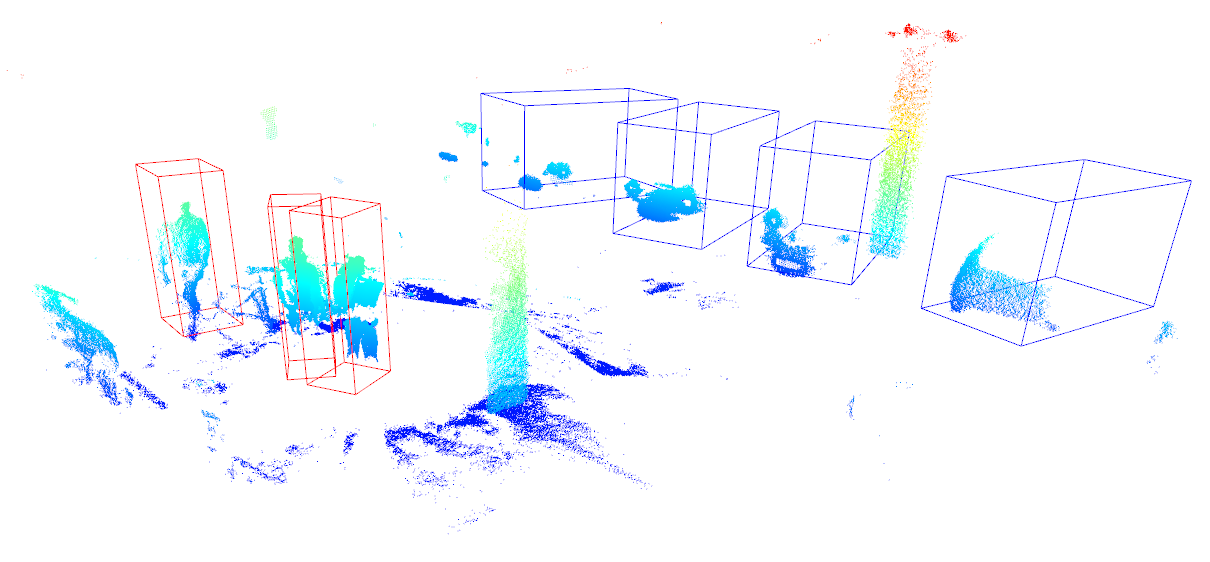
\includegraphics[width=\linewidth]{fig/snn_alfa_detections.png}
    \captionsetup{justification=centering}
    \caption{}
    \label{fig:3dscnn_pred_alfa}
\end{subfigure}
\hfill
\begin{subfigure}{0.49\textwidth}
    \centering
    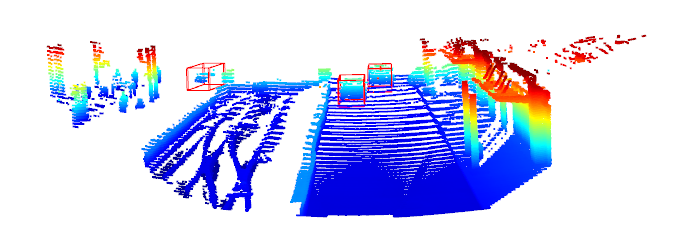
\includegraphics[width=\linewidth]{fig/snn_panda_detections.png}
    \captionsetup{justification=centering}
    \caption{}
    \label{fig:3dscnn_pred_panda}
\end{subfigure}
\caption{3D-SCNN objektu prognozes: (\textbf{a}) ToF datos, kas iegūti, apvienojot vairāku sensoru datus; (\textbf{b}) Pandaset neskenējošā LiDAR datu kopas ainā.}
\label{fig:3dscnn_preds}
\end{figure}

Modeļu apmācības rezultāti dažādās datu kopās apkopoti \ref{table:snn_map}. tabulā. Salīdzināšanai \textit{VGG-11} un \textit{VGG-13} modeļi atsevišķi apmācīti ar \textit{KITTI} un \textit{Pandaset}, pēc tam novērtēti gan attiecīgajās apmācības datu kopās, gan iegūtajos ToF datos. Mērķis bija izvērtēt to vispārināšanas spēju starp dažādām sensoru modalitātēm. Papildus modeļi salīdzināti ar modernākajiem uz LiDAR balstītajiem \Gls{snn} uztveres modeļiem \cite{Zhou2020, qiu2024}. Ar \textit{KITTI} apmācītie modeļi uzrādīja labus rezultātus pašā \textit{KITTI} datu kopā: \textit{VGG-13} sasniedza augstāku AP (75,3~\%) nekā \textit{VGG-11} (70,7~\%). Tomēr, pārbaudot tos ToF datos, novērots būtisks veiktspējas kritums, īpaši \textit{VGG-11} gadījumā (40,0~\% \textit{VGG-11} un 65,0~\% \textit{VGG-13}), uzsverot domēnu atšķirību starp LiDAR balstītajiem \textit{KITTI} datiem un ToF punktu mākoņiem. Tas liecina, ka modeļiem, kas apmācīti tikai ar LiDAR datiem, ir grūti pielāgoties ToF signālu īpašībām. Savukārt ar \textit{Pandaset} apmācītie modeļi demonstrēja vienmērīgāku veiktspēju dažādās datu kopās. Ar \textit{Pandaset} apmācītie \textit{VGG-11} un \textit{VGG-13} sasniedza attiecīgi 69,0~\% un 71,0~\% AP \textit{Pandaset} datos. Būtiski, ka apmācība ar \textit{Pandaset} uzlaboja \textit{VGG-11} ToF detektēšanas veiktspēju un nodrošināja labāku pārnesamību uz ToF datiem — 55,0~\% AP. Savukārt ar \textit{KITTI} apmācītais \textit{VGG-13} sasniedza augstāko ToF AP — 65,0~\%. Šie rezultāti liecina, ka \textit{Pandaset} uz priekšu vērstā neskenējošā LiDAR lielāka līdzība ar ToF uztveri nekā \textit{KITTI} 360 grādu LiDAR var uzlabot pārnesamību un apmācības precizitāti, taču vispārināšana starp modalitātēm var būt atkarīga gan no apmācības datu kopas, gan tīkla arhitektūras, kā \textit{VGG-13} gadījumā.

\begin{table}[ht]
\centering
\caption{Modeļu parametru, retinājuma un automobiļu klases BEV AP salīdzinājums dažādās datu kopās}
\label{table:snn_map}
\footnotesize

\setlength{\tabcolsep}{3pt}
\begin{adjustbox}{max width=\textwidth}\begin{tabular}{l c c c c c}
\toprule
\textbf{Modelis} & \textbf{Datu kopa} & \textbf{Ieeja} & \textbf{Param. sk. (M)} & \textbf{Retinājums (\%)} & \textbf{AP (\%)} \\
\midrule
\textbf{Saistītie darbi---SNN}  & & & & & \\
  Zhou u.\,c. SNN \cite{Zhou2020}  & KITTI & Vokselis & - & - & 67{,}00 \\
  Zhou u.\,c. SNN ar SC \cite{Zhou2020}  & KITTI & Vokselis & - & - & 68{,}27 \\
\midrule
\textbf{Saistītie darbi---ANN}  & & & & & \\
  PointPillar \cite{lang2019} & KITTI & Stabs & 18 & - & 86{,}48 \\
  PV-RCNN \cite{shi2020} & KITTI & PV & 50 & - & 90{,}59 \\
\midrule
\textbf{Šis darbs---SNN}  & & & & & \\
\multirow{2}{*}{\raggedright SVGG-11  (Apmācīts ar KITTI)}
    & KITTI & TVC & 12{,}8 & 55{,}73 & 70{,}7  \\
    & ToF   & TVC & 12{,}8 & 35{,}10 & 40{,}0  \\
\midrule
\multirow{2}{*}{\raggedright SVGG-13  (Apmācīts ar KITTI)}
    & KITTI & TVC & 13{,}1 &  63{,}67 & 75{,}3  \\
    & ToF   & TVC & 13{,}1 &  45{,}05 & 65{,}0  \\
\midrule
\multirow{2}{*}{\raggedright SVGG-11  (Apmācīts ar Pandaset)}
    & Pandaset & TVC & 12{,}8 & 50{,}26 & 69{,}0 \\
    & ToF      & TVC & 12{,}8 & 20{,}15 & 55{,}0 \\
\midrule
\multirow{2}{*}{\raggedright SVGG-13  (Apmācīts ar Pandaset)}
    & Pandaset & TVC & 13{,}1 & 42{,}15 & 71{,}0 \\
    & ToF      & TVC & 13{,}1 & 32{,}67 & 60{,}0 \\
\bottomrule
\end{tabular}\end{adjustbox}

\end{table}



    \paragraph{Realizācija FPGA}\mbox{} \\
    

Lai demonstrētu \Gls{snn} detektora praktisko piemērotību, impulsu konvolūcijas pamattīkls realizēts pārkonfigurējamajā \Gls{fpga} paātrinātājā, kas aprakstīts \ref{sec:fpga_impl}. apakšnodaļā. Aparatūras realizācijā izmantota tā pati tīkla topoloģija kā \textit{SpikingJelly} ietvarā izstrādātajam programmatūras modelim, lai saglabātu līdzvērtību starp programmatūras apmācību un aparatūras inferenci. Paātrinātājs atbalsta konvolūcijas slāņus ar līdz 256 ieejas un 512 izejas kanāliem, ļaujot realizēt dziļus tīklus praktiskiem lietojumiem.

Arhitektūra ir konfigurējama pazīmju kartēm līdz \(512 \times 512\) pikseļiem, kas atbilst vokseļu režģiem apkārtskata uztverei aptuveni \qty{50}{\metre} rādiusā ar horizontālo vokseļu izšķirtspēju līdz \qty{0.1}{\metre}. Tādējādi tā pati paātrinātāja arhitektūra bez aparatūras izmaiņām var izpildīt gan kompaktos novērtēšanas tīklus, gan lielākus 3D objektu detektēšanas modeļus.

\ref{fig:fpga_vs_jetson}. attēlā salīdzināts izmērītais \Gls{fpga} realizācijas inferences latentums ar ekvivalentu programmatūras realizāciju \textit{Jetson AGX Orin} GPU, kur \Gls{fpga} un \textit{Jetson} izpilda vienādu impulsu tīkla konfigurāciju ar vienādiem ieejas izmēriem un laika soļu skaitu. Norādītais \Gls{fpga} latentums aptver impulsu konvolūcijas pamattīkla izpildi un neietver ieejas vokselizāciju, \Gls{ssd} detektēšanas galvas apstrādi un ietverošo taisnstūru pēcapstrādi. Tā kā \Gls{fpga} apstrādā konvolūcijas slāņus kā konveijerizētu datu straumi, pievienojot tīklam papildu slāņus, latentums palielinās tikai nedaudz. Savukārt GPU izpildes laiks pieaug aptuveni proporcionāli tīkla dziļumam, jo katrs slānis tiek izpildīts kā atsevišķs kodols.

\begin{figure}[ht]
  \centering
  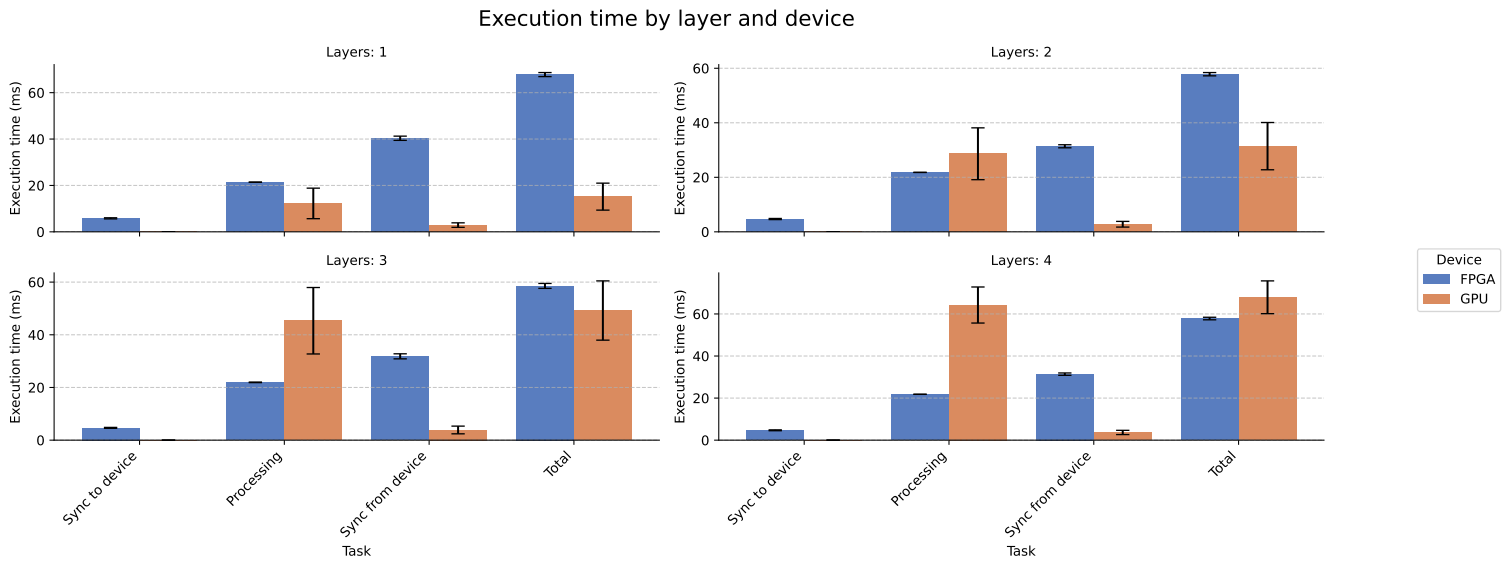
\includegraphics[width=0.9\textwidth]{fig/fpga_vs_jetson.png}
  \caption{\Gls{fpga} \Gls{snn} izpildes laiks salīdzinājumā ar ekvivalentu modeli GPU.}
  \label{fig:fpga_vs_jetson}
% \par\smallskip
% {\footnotesize \textit{Execution time by layer and device} — izpildes laiks pēc slāņu skaita un ierīces; \textit{Layers} — slāņi; \textit{Execution time} — izpildes laiks; \textit{Device} — ierīce; \textit{Sync to device} — sinhronizācija uz ierīci; \textit{Processing} — apstrāde; \textit{Sync from device} — sinhronizācija no ierīces; \textit{Total} — kopā; \textit{Task} — uzdevums.\par}
\end{figure}

Sekliem tīkliem abu platformu veiktspēja ir salīdzināma. Tomēr, palielinoties tīkla dziļumam, \Gls{fpga} konveijers tiek pilnībā noslogots un pārspēj GPU realizāciju. Novērtētajam četrslāņu tīklam kopējais inferences latentums saglabājas zem \qty{60}{\milli\second}, atbilstot reāllaika apstrādes prasībām automobiļu uztveres sistēmās.

Abās skaitļošanas platformās jaudas patēriņš uzraudzīts nepārtrauktas inferences slodzes laikā. \Gls{fpga} realizācijai \textit{Alpha Data} ražotāja nodrošinātā utilīta \texttt{avr2util} uzrādīja aptuveni 15,8~W paātrinātāja kartes jaudas patēriņu. \textit{Jetson AGX Orin} gadījumā uzraudzības utilīta \texttt{jtop} inferences laikā uzrādīja aptuveni 19,8~W, darbojoties 40~W jaudas režīmā. Tādēļ novērotā \Gls{fpga} kartes jauda pārbaudītajos apstākļos bija aptuveni par 20~\% mazāka nekā norādītā \textit{Jetson} jauda. Novērotā jaudas atšķirība jāuzskata par orientējošu pilnas ierīces līmeņa salīdzinājumu, kas ietver resursdatora sistēmas un perifērijas jaudu, nevis par tieši izmērītu \Gls{snn} paātrināšanas energoefektivitātes priekšrocību.




\section{Secinājumi un turpmākais darbs}
\subsection{Secinājumi}


Šajā promocijas darbā pētīta \Gls{snn} izmantošana efektīvai telpisku un temporālu datu apstrādei, galvenokārt pievēršoties to paātrināšanai pārkonfigurējamā aparatūrā ar \Gls{fpga}. Darbs aptver gan algoritmiskos, gan aparatūras aspektus \Gls{snn} realizācijā, piemēram, neironu modeļus, neironu tīklus, apmācības metodes, telpiski temporālu datu reprezentācijas un \Gls{fpga} paātrinātāju arhitektūras. Rezultāti demonstrē, ka \Gls{snn} nodrošina piemērotu skaitļošanas pieeju retinātiem temporāliem datiem un tos var realizēt pārkonfigurējamā aparatūrā, lai sasniegtu zema latentuma un energoefektīvu inferenci.

Pirmajā tēzē pārbaudīta \Gls{fpga} izmantošana kā pārkonfigurējama aparatūras platforma \Gls{snn} paātrināšanai. Izstrādāts pārkonfigurējams, uz PCIe balstīts \Gls{fpga} paātrinātājs konvolucionālo \Gls{snn} realizācijai. Paātrinātājs atbalsta konfigurējamus konvolūcijas slāņus un impulsu neironu modeļus dažādu \Gls{snn} arhitektūru realizācijai aparatūras platformā bez atkārtotas sintēzes. Pārbaudīts, ka kvantēšana ar mazu bitu platumu var saglabāt konvolucionālo \Gls{snn} klasifikācijas veiktspēju, vienlaikus ļaujot tos realizēt pārkonfigurējamā \Gls{fpga} paātrinātājā. Rezultāti parādīja, ka svaru precizitātes samazināšana no 32 līdz 4 bitiem saglabāja F1 rādītāju 1~\% robežās no ekvivalenta pilnas precizitātes \Gls{snn} modeļa gan \textit{MNIST}, gan četrslāņu un sešslāņu \textit{Caltech-101} modeļiem. Konkrēti, attiecīgie 4 bitu modeļi sasniedza F1 rādītājus 96,79~\%, 89,32~\% un 88,10~\%. Novērtētā realizācija demonstrēja arī mazu dinamisko jaudas patēriņu, apliecinot energoefektīvas \Gls{snn} klasifikācijas iespējamību pārkonfigurējamā aparatūrā. Eksperimentālie rezultāti ar \textit{Kintex UltraScale KU115} \Gls{fpga} parādīja, ka izmērītais vidējās dinamiskās jaudas pieaugums \Gls{fpga} inferences laikā pārbaudītajā slodzē sasniedza aptuveni 91~mW. Jaudas mērījumi arī uzsver atšķirību starp paātrinātāja aktivitāti un aparatūras platformas dīkstāves jaudas patēriņu. Vidējā jauda, kas izmērīta 12~V barošanas ķēdē dīkstāvē, bija 15,77~W. Salīdzinoši nelielais inferences jaudas pieaugums norāda, ka \Gls{snn} slodze radīja ierobežotu papildu vidējo jaudu. Salīdzinoši lielā dīkstāves jauda izskaidrojama ar lieljaudas KU115 \Gls{fpga} izstrādes kartes izmantošanu jaudas ziņā optimizētas iegultās platformas vietā. Specializēta paātrinātāja platforma ar piemērota izmēra \Gls{fpga} samazinātu šo dīkstāves patēriņu. Tomēr šādi uzlabojumi paliek turpmākā darba virziens.

Eksperimenti demonstrēja arī zema latentuma inferenci novērtētajiem konvolucionālajiem tīkliem un parādīja, ka \Gls{fpga} paātrināšana var nodrošināt determinētu konveijerizētu izpildi un latentuma uzlabojumus salīdzinājumā ar iegultām GPU platformām (piemēram, \textit{NVIDIA Jetson AGX Orin}). Eksperimenti arī demonstrēja, ka konveijerizētas \Gls{fpga} izpildes priekšrocības ir izteiktākas, ja kaskādē savienoti vairāki konvolūcijas slāņi. Salīdzinājums ar augstas veiktspējas diskrētu GPU (piemēram, \textit{NVIDIA GeForce RTX 5070 Ti}) parādīja, ka \Gls{fpga} paātrināšana ne vienmēr nodrošina visaugstāko caurlaidību. Šajā gadījumā galvenās priekšrocības ir determinēts latentums un ievērojami mazākas jaudas prasības nekā GPU platformām.

Otrajā tēzē pārbaudīta konvolucionālo \Gls{snn} piemērotība objektu detektēšanai punktu mākoņos un novērtēta to potenciālā energoefektivitāte. Eksperimentālie rezultāti demonstrēja, ka konvolucionālie \Gls{snn} spēj apstrādāt laikā kodētas 3D telpiskās reprezentācijas. Konkrēti, izstrādātā 3D-SCNN arhitektūra piemērota objektu detektēšanai LiDAR datos. Izstrādātā impulsu detektēšanas arhitektūra apvieno temporālo vokseļu kodēšanu, impulsu \textit{VGG} pamattīklu un detektēšanas galvas objektu klasifikācijai un orientētu ietverošo taisnstūru regresijai. \textit{KITTI} validācijas datu kopā \textit{VGG-13} modelis sasniedza 72,03~\% \Gls{bev} vidējo precizitāti automobiļu klasei. Papildu eksperimenti ar izkliedētu \Gls{tof} sensoru sistēmu demonstrēja praktisku piemērotību \Gls{tof} sensoru punktu mākoņu datiem. Analītisks enerģijas salīdzinājums, kas balstīts uz reprezentatīviem 45~nm CMOS operāciju enerģijas pieņēmumiem, novērtētajām \Gls{snn} arhitektūrām uzrādīja aptuveni par 27,5~\% mazāku inferences enerģiju nekā ekvivalentiem tradicionāliem \Gls{ann} modeļiem. Eksperimenti demonstrēja, ka uz \Gls{snn} balstīti modeļi var iegūt telpiskas un temporālas pazīmes no retinātiem 3D sensoru datiem, kas kodēti uz notikumiem balstītā reprezentācijā, lai veiktu objektu detektēšanu un izmantotu energoefektīvas notikumu apstrādes priekšrocības.

Tomēr piedāvātajam 3D-SCNN ir noteikti ierobežojumi. Parādīts, ka \Gls{snn} efektivitātes priekšrocības ir stipri atkarīgas no impulsu retinājuma un simulācijas laika soļu skaita. Atšķirībā no tradicionālajiem \Gls{ann}, kuros aritmētisko operāciju skaitu nosaka tīkla arhitektūra, \Gls{snn} operāciju skaits papildus ir atkarīgs no ģenerēto impulsu skaita. Tādējādi reta impulsu aktivitāte var būtiski samazināt operāciju skaitu. Tomēr rezultāti arī parāda, ka retinātu aprēķinu ieguvumu var kompensēt atmiņas piekļuves, īpaši tad, ja neironu stāvokļi tiek glabāti ārējā SDRAM atmiņā. Tādēļ efektīva atmiņas shēma un mikroshēmas iekšējās \Gls{bram} izmantošana ir būtiska \Gls{snn} potenciālo priekšrocību īstenošanai.

Turklāt piedāvātās 3D-SCNN detektēšanas arhitektūras novērtētie enerģijas ietaupījumi vēl nav pārbaudīti ar pilnībā realizēta modeļa fiziskiem jaudas mērījumiem. Turpmākajā darbā joprojām nepieciešama impulsu pamattīkla, pazīmju piramīdas starpposma un detektēšanas galvas posmu pilnīga realizācija aparatūras platformā, kam sekotu jaudas patēriņa mērījumi.

Trešajā tēzē pārbaudīta konveijerizēta, pārkonfigurējama \Gls{fpga} paātrinātāja iespējamība ar jauktu atmiņas shēmu, kur svari tiek glabāti mikroshēmā un neironu membrānas potenciāli — ārpus tās. Šī izvēle risina ierobežotas iekšējās atmiņas problēmu, realizējot dziļākus konvolucionālos \Gls{snn}, vienlaikus saglabājot elastību dažādām tīklu konfigurācijām. Novērtētajiem četrslāņu un sešslāņu \textit{Caltech-101} tīkliem novērtētās mikroshēmas iekšējās atmiņas prasības samazinātas attiecīgi aptuveni par 53,8~\% un 55,0~\% salīdzinājumā ar ekvivalentām konfigurācijām, kur visa atmiņa izvietota mikroshēmā. Turklāt noteikts, ka novērtētie četrslāņu un sešslāņu tīkli sasniedza attiecīgi 2,43~ms un 2,81~ms inferences latentumu, parādot, ka membrānas potenciālu atmiņas pārvietošana ārpus mikroshēmas saglabā zemu inferences latentumu. Papildu eksperimenti demonstrēja arī konveijerizētas izpildes priekšrocības dziļākām tīkla konfigurācijām un apstiprināja arhitektūras piemērotību zema latentuma un determinētai \Gls{snn} inferencei.

Kopumā rezultāti apstiprina promocijas darba mērķa sasniegšanu un demonstrē, ka kvantētu \Gls{snn} modeļu inferenci un membrānas potenciālu ārēju glabāšanu var apvienot efektīvai resursu izmantošanai. Turklāt piedāvātais risinājums līdzsvaro pārkonfigurējamību, mērogojamību un energoefektivitāti uz \Gls{fpga} balstītā neiromorfajā skaitļošanā. Uz notikumiem balstītu \Gls{snn} realizācija retinātu telpiski temporālu datu apstrādei un to ieviešana pārkonfigurējamā aparatūrā nodrošina īstenojamu pieeju mazas jaudas inferencei perifērijas ierīcēs. Tomēr saglabājas vairāki ierobežojumi. Jo īpaši novērtēto punktu mākoņu \Gls{snn} modeļu detektēšanas precizitāte ir zemāka nekā tradicionālajiem \Gls{ann} modeļiem ar sarežģītākām arhitektūrām. Arī \Gls{snn} efektivitātes priekšrocības ir atkarīgas no vairākiem faktoriem, piemēram, impulsu retinājuma, kodēšanas laika soļa ilguma, kvantēšanas un atmiņas arhitektūras. Tādēļ efektīvai \Gls{snn} inferencei nepieciešama kopīga neironu tīkla modeļa, datu reprezentācijas un aparatūras paātrinātāja realizācijas optimizācija.

\subsection{Turpmākais darbs}


Turpmākajā darbā iespējami vairāki virzieni piedāvāto \Gls{snn} modeļu un uz \Gls{fpga} balstītā \Gls{snn} paātrinātāja veiktspējas, mērogojamības, efektivitātes un piemērojamības uzlabošanai.

Pirmkārt, dažos uzdevumos impulsu modeļu precizitāte joprojām atpaliek no tradicionālajiem \Gls{ann}. Turpmāk varētu pētīt progresīvākas \Gls{snn} arhitektūras un apmācības metodes; paātrinātāja paplašināšana atlikuma savienojumu vai uz transformeriem balstītu modeļu atbalstam palielinātu tā piemērojamību dažādām \Gls{snn} arhitektūrām.

Otrkārt, varētu veikt kopīgu neironu tīkla un aparatūras arhitektūras optimizāciju. Turpmākajās realizācijās varētu pētīt neironu stāvokļu un starpposmu pazīmju karšu saspiešanu. Saspiestu neironu stāvokļu ar mazu bitu platumu glabāšana mikroshēmā varētu samazināt ar atmiņas piekļuvi saistīto jaudas patēriņu. Šim nolūkam varētu izmantot evolucionārās apmācības metodes un aparatūru ievērojošu \Gls{nas}, lai meklētu tīkla konfigurācijas ar labāku kompromisu starp precizitāti, resursu izmantojumu un enerģijas patēriņu.

Līdzīgi dažus no šiem ierobežojumiem var mazināt, integrējot lielāku datu apstrādes konveijera daļu \Gls{fpga} paātrinātājā vai ciešāk integrējot to ar attēlveidošanas sensoriem, samazinot dārgas pārsūtīšanas starp resursdatora procesoru, ārējo atmiņu un \Gls{fpga}. Tas varētu ietvert vokselizācijas, impulsu kodēšanas un objektu detektora galvas daļu aparatūras realizāciju. Tāpat LiDAR vai \Gls{spad} sensoru izeju tieša apstrāde \Gls{fpga} varētu samazināt starpposmu histogrammu veidošanu un \Gls{tdc} apstrādi, savukārt ciešāka integrācija ar notikumu kamerām varētu ļaut paātrinātājam tieši apstrādāt asinhronus notikumus.

Vēl viens turpmākais virziens ir sensoru sistēmas, \Gls{snn} modeļu un paātrinātāja integrācija automatizētas braukšanas vai citās iegultās skaitļošanas platformās. Lai gan pašreizējais darbs demonstrē reālu sensoru datu inferences iespējamību ar \Gls{snn} \Gls{fpga} aparatūrā, integrācija ar automatizētas braukšanas ietvariem ļautu novērtēt pilnu uztveres un lēmumu pieņemšanas konveijeru.

Pašreizējie rezultāti norāda uz lielu potenciālu turpmākajās \Gls{snn} realizācijās un to paātrināšanā ar \Gls{fpga}, īpaši tad, ja notikumu sensori integrēti pilnīgā sistēmā, kur uztvere, neirālā apstrāde un aparatūras arhitektūra projektētas kopīgi.



\printbibliography[heading=bibintoc,title={LITERATŪRAS SARAKSTS}]


\end{document}
